% NGÂN HÀNG TUYỂN SINH 10 – BÀI 1

\begin{bt}%[TS10 1.0 1.2]%[ma:654bf2ee]
Cho parabol $(P): y = \frac{1}{2}x^2$.
\textbf{a)} Vẽ đồ thị $(P)$ trên hệ trục tọa độ. \par
\textbf{b)} Tìm tọa độ các điểm $M$ thuộc $(P)$ (khác gốc tọa độ $O$) sao cho tung độ của điểm $M$ gấp đôi hoành độ của nó.
\loigiai{
\textbf{a)} Vẽ đồ thị $(P): y = \frac{1}{2}x^2$ \hfill \textit{(1,0 điểm)} \par
Bảng giá trị:
\begin{center}
\begin{tabular}{|c|c|c|c|c|c|}
\hline
$x$ & $-4$ & $-2$ & $0$ & $2$ & $4$ \\
\hline
$y = \frac{1}{2}x^2$ & $8$ & $2$ & $0$ & $2$ & $8$ \\
\hline
\end{tabular}
\end{center}
Đồ thị hàm số $(P)$ là một đường parabol đi qua gốc tọa độ $O$, nhận trục $Oy$ làm trục đối xứng và nằm phía trên trục hoành.
\begin{center}
\begin{tikzpicture}[>=stealth, scale=0.7]
\draw[->] (-5.5,0) -- (5.5,0) node[below] {$x$};
\draw[->] (0,-1) -- (0,9.5) node[left] {$y$};
\fill (0,0) circle (1.5pt) node[below right] {$O$};
\draw[domain=-4.2:4.2, smooth, thick] plot (\x, {0.5*\x*\x});
\draw[dashed] (-4,0) node[below]{$-4$} |- (0,8) node[above left]{$8$} -| (4,0) node[below]{$4$};
\draw[dashed] (-2,0) node[below]{$-2$} |- (0,2) node[above left]{$2$} -| (2,0) node[below]{$2$};
\fill (-4,8) circle (1.5pt); \fill (4,8) circle (1.5pt);
\fill (-2,2) circle (1.5pt); \fill (2,2) circle (1.5pt);
\node[right] at (4.2, 8.8) {$(P)$};
\end{tikzpicture}
\end{center}
\textbf{b)} Tìm tọa độ các điểm $M$ \hfill \textit{(0,5 điểm)} \par
Vì $M$ thuộc $(P)$ nên tọa độ của $M$ có dạng $M\left(x_M; \frac{1}{2}x_M^2\right)$. \par
Theo đề bài, tung độ gấp đôi hoành độ nên ta có phương trình:
$$ \frac{1}{2}x_M^2 = 2x_M $$
$$ \Leftrightarrow x_M^2 - 4x_M = 0 $$
$$ \Leftrightarrow x_M(x_M - 4) = 0 $$
$$ \Leftrightarrow \heva{&x_M = 0 \\ &x_M = 4} $$
Với $x_M = 0 \Rightarrow y_M = 0$, ta được điểm $(0; 0)$ (loại vì $M$ khác gốc tọa độ). \par
Với $x_M = 4 \Rightarrow y_M = \frac{1}{2} \cdot 4^2 = 8$, ta được điểm $M(4; 8)$ (nhận). \par
Vậy tọa độ điểm $M$ cần tìm là $M(4; 8)$.
}
\end{bt}

\begin{bt}%[TS10 1.0 1.1]%[ma:26b15222]
Cho parabol $(P): y = -\frac{1}{4}x^2$.
\textbf{a)} Vẽ đồ thị $(P)$ trên hệ trục tọa độ. \par
\textbf{b)} Tìm tọa độ những điểm $A$ thuộc $(P)$ biết tung độ của điểm đó bằng $-9$.
\loigiai{
\textbf{a)} Vẽ đồ thị $(P): y = -\frac{1}{4}x^2$ \hfill \textit{(1,0 điểm)} \par
Bảng giá trị:
\begin{center}
\begin{tabular}{|c|c|c|c|c|c|}
\hline
$x$ & $-4$ & $-2$ & $0$ & $2$ & $4$ \\
\hline
$y = -\frac{1}{4}x^2$ & $-4$ & $-1$ & $0$ & $-1$ & $-4$ \\
\hline
\end{tabular}
\end{center}
Đồ thị hàm số $(P)$ là một đường parabol đi qua gốc tọa độ $O$, nhận trục $Oy$ làm trục đối xứng và nằm phía dưới trục hoành.
\begin{center}
\begin{tikzpicture}[>=stealth, scale=0.8]
\draw[->] (-5.5,0) -- (5.5,0) node[above] {$x$};
\draw[->] (0,-5.5) -- (0,1) node[right] {$y$};
\fill (0,0) circle (1.5pt) node[above right] {$O$};
\draw[domain=-4.5:4.5, smooth, thick] plot (\x, {-0.25*\x*\x});
\draw[dashed] (-4,0) node[above]{$-4$} |- (0,-4) node[below left]{$-4$} -| (4,0) node[above]{$4$};
\draw[dashed] (-2,0) node[above]{$-2$} |- (0,-1) node[below left]{$-1$} -| (2,0) node[above]{$2$};
\fill (-4,-4) circle (1.5pt); \fill (4,-4) circle (1.5pt);
\fill (-2,-1) circle (1.5pt); \fill (2,-1) circle (1.5pt);
\node[right] at (4.5, -5) {$(P)$};
\end{tikzpicture}
\end{center}
\textbf{b)} Tìm tọa độ những điểm $A$ \hfill \textit{(0,5 điểm)} \par
Gọi tọa độ điểm $A$ là $(x_A; y_A)$. Vì $A$ thuộc $(P)$ và có tung độ $y_A = -9$ nên ta có:
$$ -\frac{1}{4}x_A^2 = -9 $$
$$ \Leftrightarrow x_A^2 = 36 $$
$$ \Leftrightarrow x_A = 6 \text{ hoặc } x_A = -6 $$
Với $x_A = 6$, ta có điểm $A_1(6; -9)$. \par
Với $x_A = -6$, ta có điểm $A_2(-6; -9)$. \par
Vậy có hai điểm $A$ thỏa mãn yêu cầu bài toán là $(6; -9)$ và $(-6; -9)$.
}
\end{bt}

\begin{bt}%[TS10 1.0 1.3]%[ma:7fad95b9]
Cho parabol $(P): y = x^2$.
\textbf{a)} Vẽ đồ thị $(P)$ trên mặt phẳng tọa độ. \par
\textbf{b)} Tìm tọa độ các điểm $B$ thuộc $(P)$ sao cho tổng hoành độ và tung độ của điểm đó bằng $12$.
\loigiai{
\textbf{a)} Vẽ đồ thị $(P): y = x^2$ \hfill \textit{(1,0 điểm)} \par
Bảng giá trị:
\begin{center}
\begin{tabular}{|c|c|c|c|c|c|}
\hline
$x$ & $-2$ & $-1$ & $0$ & $1$ & $2$ \\
\hline
$y = x^2$ & $4$ & $1$ & $0$ & $1$ & $4$ \\
\hline
\end{tabular}
\end{center}
Đồ thị hàm số $(P)$ là một đường parabol đi qua gốc tọa độ $O$, nhận trục $Oy$ làm trục đối xứng và nằm phía trên trục hoành.
\begin{center}
\begin{tikzpicture}[>=stealth, scale=1]
\draw[->] (-3.5,0) -- (3.5,0) node[below] {$x$};
\draw[->] (0,-1) -- (0,5.5) node[left] {$y$};
\fill (0,0) circle (1.5pt) node[below right] {$O$};
\draw[domain=-2.2:2.2, smooth, thick] plot (\x, {\x*\x});
\draw[dashed] (-2,0) node[below]{$-2$} |- (0,4) node[above left]{$4$} -| (2,0) node[below]{$2$};
\draw[dashed] (-1,0) node[below]{$-1$} |- (0,1) node[above left]{$1$} -| (1,0) node[below]{$1$};
\fill (-2,4) circle (1.5pt); \fill (2,4) circle (1.5pt);
\fill (-1,1) circle (1.5pt); \fill (1,1) circle (1.5pt);
\node[right] at (2.2, 4.8) {$(P)$};
\end{tikzpicture}
\end{center}
\textbf{b)} Tìm tọa độ các điểm $B$ \hfill \textit{(0,5 điểm)} \par
Gọi tọa độ điểm $B$ là $(x_B; y_B)$. Vì $B \in (P)$ nên $y_B = x_B^2$. \par
Theo đề bài, tổng hoành độ và tung độ bằng $12$, ta có phương trình:
$$ x_B + y_B = 12 $$
$$ \Leftrightarrow x_B + x_B^2 = 12 $$
$$ \Leftrightarrow x_B^2 + x_B - 12 = 0 $$
$$ \Leftrightarrow x_B^2 - 3x_B + 4x_B - 12 = 0 $$
$$ \Leftrightarrow x_B(x_B - 3) + 4(x_B - 3) = 0 $$
$$ \Leftrightarrow (x_B - 3)(x_B + 4) = 0 $$
$$ \Leftrightarrow \heva{&x_B = 3 \\ &x_B = -4} $$
Với $x_B = 3 \Rightarrow y_B = 3^2 = 9$, ta được điểm $B_1(3; 9)$. \par
Với $x_B = -4 \Rightarrow y_B = (-4)^2 = 16$, ta được điểm $B_2(-4; 16)$. \par
Vậy tọa độ các điểm $B$ cần tìm là $(3; 9)$ và $(-4; 16)$.
}
\end{bt}

\begin{bt}%[TS10 1.0 1.4]%[ma:f6439493]
Cho parabol $(P): y = -x^2$ và đường thẳng $(d): y = -3x + 2$.
\textbf{a)} Vẽ đồ thị $(P)$ trên hệ trục tọa độ. \par
\textbf{b)} Tìm tọa độ giao điểm của $(P)$ và $(d)$ bằng phép tính.
\loigiai{
\textbf{a)} Vẽ đồ thị $(P): y = -x^2$ \hfill \textit{(1,0 điểm)} \par
Bảng giá trị:
\begin{center}
\begin{tabular}{|c|c|c|c|c|c|}
\hline
$x$ & $-2$ & $-1$ & $0$ & $1$ & $2$ \\
\hline
$y = -x^2$ & $-4$ & $-1$ & $0$ & $-1$ & $-4$ \\
\hline
\end{tabular}
\end{center}
Đồ thị hàm số $(P)$ là một đường parabol đi qua gốc tọa độ $O$, nhận trục $Oy$ làm trục đối xứng và nằm phía dưới trục hoành.
\begin{center}
\begin{tikzpicture}[>=stealth, scale=1]
\draw[->] (-3.5,0) -- (3.5,0) node[above] {$x$};
\draw[->] (0,-5.5) -- (0,1) node[right] {$y$};
\fill (0,0) circle (1.5pt) node[above right] {$O$};
\draw[domain=-2.2:2.2, smooth, thick] plot (\x, {-\x*\x});
\draw[dashed] (-2,0) node[above]{$-2$} |- (0,-4) node[below left]{$-4$} -| (2,0) node[above]{$2$};
\draw[dashed] (-1,0) node[above]{$-1$} |- (0,-1) node[below left]{$-1$} -| (1,0) node[above]{$1$};
\fill (-2,-4) circle (1.5pt); \fill (2,-4) circle (1.5pt);
\fill (-1,-1) circle (1.5pt); \fill (1,-1) circle (1.5pt);
\node[right] at (2.2, -4.8) {$(P)$};
\end{tikzpicture}
\end{center}
\textbf{b)} Tìm tọa độ giao điểm của $(P)$ và $(d)$ \hfill \textit{(0,5 điểm)} \par
Phương trình hoành độ giao điểm của $(P)$ và $(d)$ là:
$$ -x^2 = -3x + 2 $$
$$ \Leftrightarrow x^2 - 3x + 2 = 0 $$
Vì $a + b + c = 1 + (-3) + 2 = 0$ nên phương trình có hai nghiệm:
$$ x_1 = 1; \quad x_2 = 2 $$
Với $x = 1 \Rightarrow y = -(1)^2 = -1$. Ta được giao điểm thứ nhất là $(1; -1)$. \par
Với $x = 2 \Rightarrow y = -(2)^2 = -4$. Ta được giao điểm thứ hai là $(2; -4)$. \par
Vậy tọa độ giao điểm của $(P)$ và $(d)$ là $(1; -1)$ và $(2; -4)$.
}
\end{bt}

\begin{bt}%[TS10 1.0 1.5]%[ma:517c9697]
Cho parabol $(P): y = 2x^2$.
\textbf{a)} Vẽ đồ thị $(P)$ trên hệ trục tọa độ. \par
\textbf{b)} Bằng phép tính, hãy kiểm tra xem các điểm $C(3; 18)$ và $D(-2; 10)$ có thuộc đồ thị $(P)$ hay không?
\loigiai{
\textbf{a)} Vẽ đồ thị $(P): y = 2x^2$ \hfill \textit{(1,0 điểm)} \par
Bảng giá trị:
\begin{center}
\begin{tabular}{|c|c|c|c|c|c|}
\hline
$x$ & $-2$ & $-1$ & $0$ & $1$ & $2$ \\
\hline
$y = 2x^2$ & $8$ & $2$ & $0$ & $2$ & $8$ \\
\hline
\end{tabular}
\end{center}
Đồ thị hàm số $(P)$ là một đường parabol đi qua gốc tọa độ $O$, nhận trục $Oy$ làm trục đối xứng và nằm phía trên trục hoành.
\begin{center}
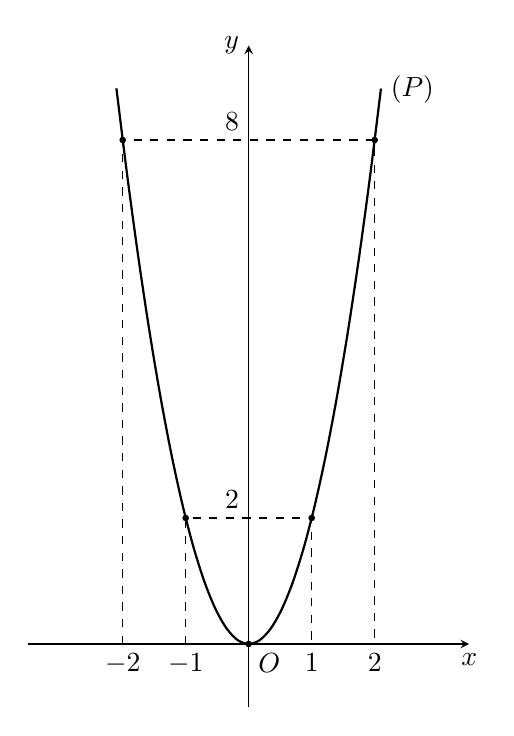
\begin{tikzpicture}[>=stealth, scale=0.8]
\draw[->] (-3.5,0) -- (3.5,0) node[below] {$x$};
\draw[->] (0,-1) -- (0,9.5) node[left] {$y$};
\fill (0,0) circle (1.5pt) node[below right] {$O$};
\draw[domain=-2.1:2.1, smooth, thick] plot (\x, {2*\x*\x});
\draw[dashed] (-2,0) node[below]{$-2$} |- (0,8) node[above left]{$8$} -| (2,0) node[below]{$2$};
\draw[dashed] (-1,0) node[below]{$-1$} |- (0,2) node[above left]{$2$} -| (1,0) node[below]{$1$};
\fill (-2,8) circle (1.5pt); \fill (2,8) circle (1.5pt);
\fill (-1,2) circle (1.5pt); \fill (1,2) circle (1.5pt);
\node[right] at (2.1, 8.8) {$(P)$};
\end{tikzpicture}
\end{center}
\textbf{b)} Kiểm tra các điểm $C(3; 18)$ và $D(-2; 10)$ \hfill \textit{(0,5 điểm)} \par
Xét điểm $C(3; 18)$, thay $x = 3$ vào hàm số của $(P)$, ta được:
$$ y = 2 \cdot 3^2 = 2 \cdot 9 = 18 $$
Giá trị này bằng với tung độ của điểm $C$ nên điểm $C(3; 18)$ thuộc $(P)$. \par
Xét điểm $D(-2; 10)$, thay $x = -2$ vào hàm số của $(P)$, ta được:
$$ y = 2 \cdot (-2)^2 = 2 \cdot 4 = 8 $$
Giá trị này khác với tung độ của điểm $D$ ($8 \neq 10$) nên điểm $D(-2; 10)$ không thuộc $(P)$. \par
Vậy điểm $C(3; 18)$ thuộc $(P)$ và điểm $D(-2; 10)$ không thuộc $(P)$.
}
\end{bt}


\begin{bt}%[TS10 1.0 1.2]%[ma:fd442b83]
Cho parabol $(P): y = \frac{1}{2}x^2$.
\textbf{a)} Vẽ đồ thị $(P)$ trên mặt phẳng tọa độ. \par
\textbf{b)} Tìm tọa độ các điểm $M$ thuộc $(P)$ sao cho tung độ của $M$ gấp đôi hoành độ.
\loigiai{
\textbf{a)} Vẽ đồ thị $(P)$ \hfill \textit{(1,0 điểm)} \par
Bảng giá trị:
\begin{center}
\begin{tabular}{|c|c|c|c|c|c|}
\hline
$x$ & $-4$ & $-2$ & $0$ & $2$ & $4$ \\
\hline
$y = \frac{1}{2}x^2$ & $8$ & $2$ & $0$ & $2$ & $8$ \\
\hline
\end{tabular}
\end{center}
Đồ thị hàm số $(P)$ là đường parabol đi qua gốc tọa độ $O$, nhận trục $Oy$ làm trục đối xứng và nằm phía trên trục hoành.
\begin{center}
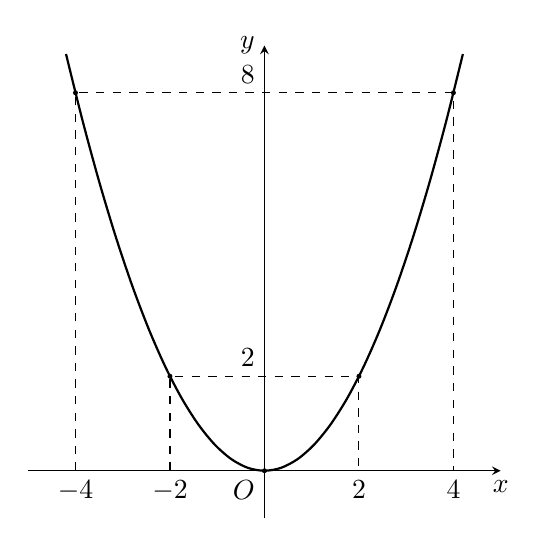
\begin{tikzpicture}[>=stealth, scale=0.6]
\draw[->] (-5,0) -- (5,0) node[below] {$x$};
\draw[->] (0,-1) -- (0,9) node[left] {$y$};
\fill (0,0) circle (1.5pt) node[below left] {$O$};
\draw[domain=-4.2:4.2, smooth, thick] plot (\x, {0.5*\x*\x});
\draw[dashed] (-4,0) node[below]{$-4$} |- (0,8) node[above left]{$8$} -| (4,0) node[below]{$4$};
\draw[dashed] (-2,0) node[below]{$-2$} |- (0,2) node[above left]{$2$} -| (2,0) node[below]{$2$};
\fill (-4,8) circle (1.5pt); \fill (4,8) circle (1.5pt);
\fill (-2,2) circle (1.5pt); \fill (2,2) circle (1.5pt);
\end{tikzpicture}
\end{center}
\textbf{b)} Tìm tọa độ các điểm $M$ \hfill \textit{(0,5 điểm)} \par
Gọi tọa độ điểm $M$ là $(x_M; y_M)$. Vì $M$ thuộc $(P)$ nên $y_M = \frac{1}{2}x_M^2$. \par
Theo đề bài, tung độ gấp đôi hoành độ nên ta có phương trình:
$$ \frac{1}{2}x_M^2 = 2x_M $$
$$ \Leftrightarrow x_M^2 - 4x_M = 0 $$
$$ \Leftrightarrow x_M(x_M - 4) = 0 $$
$$ \Leftrightarrow \heva{&x_M = 0 \\ &x_M = 4} $$
Với $x_M = 0 \Rightarrow y_M = 0$, ta được điểm $M_1(0; 0)$[cite: 1]. \par
Với $x_M = 4 \Rightarrow y_M = 8$, ta được điểm $M_2(4; 8)$. \par
Vậy tọa độ các điểm cần tìm là $(0; 0)$ và $(4; 8)$.
}
\end{bt}

\begin{bt}%[TS10 1.0 1.2]%[ma:b8626379]
Cho hàm số $y = -\frac{1}{2}x^2$ có đồ thị là $(P)$.
\textbf{a)} Vẽ đồ thị $(P)$ trên hệ trục tọa độ. \par
\textbf{b)} Tìm các điểm $A$ thuộc đồ thị $(P)$ sao cho hoành độ và tung độ của điểm đó là hai số đối nhau.
\loigiai{
\textbf{a)} Vẽ đồ thị $(P)$ \hfill \textit{(1,0 điểm)} \par
Bảng giá trị:
\begin{center}
\begin{tabular}{|c|c|c|c|c|c|}
\hline
$x$ & $-4$ & $-2$ & $0$ & $2$ & $4$ \\
\hline
$y = -\frac{1}{2}x^2$ & $-8$ & $-2$ & $0$ & $-2$ & $-8$ \\
\hline
\end{tabular}
\end{center}
Đồ thị hàm số $(P)$ là đường parabol đi qua gốc tọa độ $O$, nhận trục $Oy$ làm trục đối xứng và nằm phía dưới trục hoành.
\begin{center}
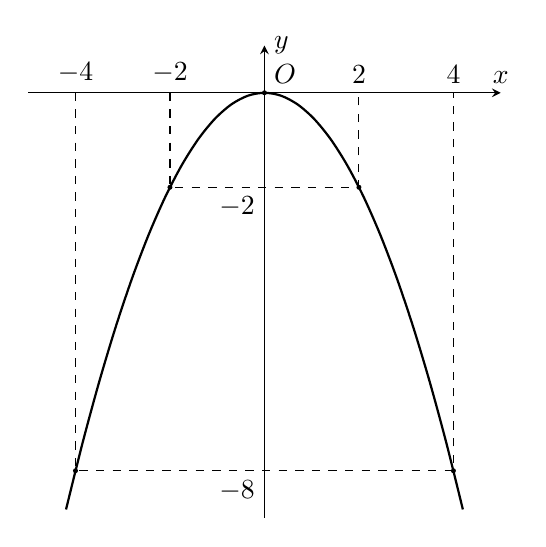
\begin{tikzpicture}[>=stealth, scale=0.6]
\draw[->] (-5,0) -- (5,0) node[above] {$x$};
\draw[->] (0,-9) -- (0,1) node[right] {$y$};
\fill (0,0) circle (1.5pt) node[above right] {$O$};
\draw[domain=-4.2:4.2, smooth, thick] plot (\x, {-0.5*\x*\x});
\draw[dashed] (-4,0) node[above]{$-4$} |- (0,-8) node[below left]{$-8$} -| (4,0) node[above]{$4$};
\draw[dashed] (-2,0) node[above]{$-2$} |- (0,-2) node[below left]{$-2$} -| (2,0) node[above]{$2$};
\fill (-4,-8) circle (1.5pt); \fill (4,-8) circle (1.5pt);
\fill (-2,-2) circle (1.5pt); \fill (2,-2) circle (1.5pt);
\end{tikzpicture}
\end{center}
\textbf{b)} Tìm các điểm $A$ \hfill \textit{(0,5 điểm)} \par
Gọi tọa độ điểm $A$ là $(x_A; y_A)$. Vì $A \in (P)$ nên $y_A = -\frac{1}{2}x_A^2$. \par
Theo đề bài, hoành độ và tung độ là hai số đối nhau nên $y_A = -x_A$. \par
Ta có phương trình:
$$ -\frac{1}{2}x_A^2 = -x_A $$
$$ \Leftrightarrow x_A^2 - 2x_A = 0 $$
$$ \Leftrightarrow x_A(x_A - 2) = 0 $$
$$ \Leftrightarrow \heva{&x_A = 0 \\ &x_A = 2} $$
Với $x_A = 0 \Rightarrow y_A = 0$, ta được điểm $A_1(0; 0)$[cite: 1, 10]. \par
Với $x_A = 2 \Rightarrow y_A = -2$, ta được điểm $A_2(2; -2)$. \par
Vậy tọa độ các điểm cần tìm là $(0; 0)$ và $(2; -2)$.
}
\end{bt}

\begin{bt}%[TS10 1.0 1.1]%[ma:e2995c57]
Cho parabol $(P): y = -2x^2$.
\textbf{a)} Vẽ đồ thị $(P)$ trên hệ trục tọa độ. \par
\textbf{b)} Tìm các điểm thuộc đồ thị $(P)$ có tung độ bằng $-8$.
\loigiai{
\textbf{a)} Vẽ đồ thị $(P)$ \hfill \textit{(1,0 điểm)} \par
Bảng giá trị:
\begin{center}
\begin{tabular}{|c|c|c|c|c|c|}
\hline
$x$ & $-2$ & $-1$ & $0$ & $1$ & $2$ \\
\hline
$y = -2x^2$ & $-8$ & $-2$ & $0$ & $-2$ & $-8$ \\
\hline
\end{tabular}
\end{center}
Đồ thị hàm số $(P)$ là đường parabol đi qua gốc tọa độ $O$, nhận trục $Oy$ làm trục đối xứng và nằm phía dưới trục hoành.
\begin{center}
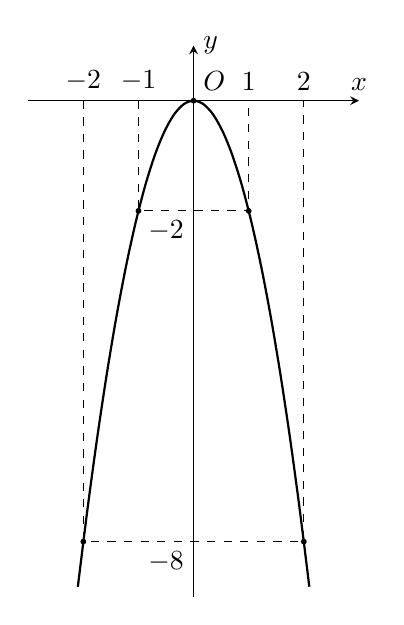
\begin{tikzpicture}[>=stealth, scale=0.7]
\draw[->] (-3,0) -- (3,0) node[above] {$x$};
\draw[->] (0,-9) -- (0,1) node[right] {$y$};
\fill (0,0) circle (1.5pt) node[above right] {$O$};
\draw[domain=-2.1:2.1, smooth, thick] plot (\x, {-2*\x*\x});
\draw[dashed] (-2,0) node[above]{$-2$} |- (0,-8) node[below left]{$-8$} -| (2,0) node[above]{$2$};
\draw[dashed] (-1,0) node[above]{$-1$} |- (0,-2) node[below left]{$-2$} -| (1,0) node[above]{$1$};
\fill (-2,-8) circle (1.5pt); \fill (2,-8) circle (1.5pt);
\fill (-1,-2) circle (1.5pt); \fill (1,-2) circle (1.5pt);
\end{tikzpicture}
\end{center}
\textbf{b)} Tìm các điểm thuộc $(P)$ \hfill \textit{(0,5 điểm)} \par
Gọi điểm cần tìm là $M(x_M; y_M)$. Vì $M \in (P)$ và có tung độ $y_M = -8$ nên ta có phương trình:
$$ -2x_M^2 = -8 $$
$$ \Leftrightarrow x_M^2 = 4 $$
$$ \Leftrightarrow x_M = 2 \text{ hoặc } x_M = -2 $$
Với $x_M = 2$, ta được điểm $(2; -8)$. \par
Với $x_M = -2$, ta được điểm $(-2; -8)$. \par
Vậy có hai điểm thỏa mãn yêu cầu bài toán là $(2; -8)$ và $(-2; -8)$[cite: 1, 34].
}
\end{bt}

\begin{bt}%[TS10 1.0 1.2]%[ma:c5303a6d]
Cho hàm số $y = \frac{1}{4}x^2$ có đồ thị là $(P)$.
\textbf{a)} Vẽ $(P)$ trên hệ trục tọa độ. \par
\textbf{b)} Tìm các điểm trên $(P)$ (khác gốc tọa độ) cách đều hai trục tọa độ.
\loigiai{
\textbf{a)} Vẽ đồ thị $(P)$ \hfill \textit{(1,0 điểm)} \par
Bảng giá trị:
\begin{center}
\begin{tabular}{|c|c|c|c|c|c|}
\hline
$x$ & $-4$ & $-2$ & $0$ & $2$ & $4$ \\
\hline
$y = \frac{1}{4}x^2$ & $4$ & $1$ & $0$ & $1$ & $4$ \\
\hline
\end{tabular}
\end{center}
Đồ thị hàm số $(P)$ là đường parabol đi qua gốc tọa độ $O$, nhận trục $Oy$ làm trục đối xứng và nằm phía trên trục hoành.
\begin{center}
\begin{tikzpicture}[>=stealth, scale=0.8]
\draw[->] (-5,0) -- (5,0) node[below] {$x$};
\draw[->] (0,-1) -- (0,5) node[left] {$y$};
\fill (0,0) circle (1.5pt) node[below left] {$O$};
\draw[domain=-4.2:4.2, smooth, thick] plot (\x, {0.25*\x*\x});
\draw[dashed] (-4,0) node[below]{$-4$} |- (0,4) node[above left]{$4$} -| (4,0) node[below]{$4$};
\draw[dashed] (-2,0) node[below]{$-2$} |- (0,1) node[above left]{$1$} -| (2,0) node[below]{$2$};
\fill (-4,4) circle (1.5pt); \fill (4,4) circle (1.5pt);
\fill (-2,1) circle (1.5pt); \fill (2,1) circle (1.5pt);
\end{tikzpicture}
\end{center}
\textbf{b)} Tìm các điểm cách đều hai trục tọa độ \hfill \textit{(0,5 điểm)} \par
Gọi tọa độ điểm cần tìm là $B(x_B; y_B)$. Vì $B \in (P)$ nên $y_B = \frac{1}{4}x_B^2$. \par
Vì điểm $B$ cách đều hai trục tọa độ nên $|x_B| = |y_B|$[cite: 33]. \par
Trường hợp 1: $y_B = x_B$
$$ \frac{1}{4}x_B^2 = x_B \Leftrightarrow x_B^2 - 4x_B = 0 \Leftrightarrow \heva{&x_B = 0 \\ &x_B = 4} $$
Do $B$ khác gốc tọa độ nên nhận $x_B = 4 \Rightarrow y_B = 4$. Ta được điểm $B_1(4; 4)$[cite: 33]. \par
Trường hợp 2: $y_B = -x_B$
$$ \frac{1}{4}x_B^2 = -x_B \Leftrightarrow x_B^2 + 4x_B = 0 \Leftrightarrow \heva{&x_B = 0 \\ &x_B = -4} $$
Do $B$ khác gốc tọa độ nên nhận $x_B = -4 \Rightarrow y_B = 4$. Ta được điểm $B_2(-4; 4)$[cite: 33]. \par
Vậy các điểm cần tìm là $(4; 4)$ và $(-4; 4)$.
}
\end{bt}

\begin{bt}%[TS10 1.0 1.1]%[ma:a731a6a9]
Cho hàm số $y = 2x^2$ có đồ thị là parabol $(P)$.
\textbf{a)} Vẽ đồ thị $(P)$ trên mặt phẳng tọa độ $Oxy$. \par
\textbf{b)} Tìm tọa độ những điểm thuộc $(P)$ có tung độ bằng $18$.
\loigiai{
\textbf{a)} Vẽ đồ thị $(P)$ \hfill \textit{(1,0 điểm)} \par
Bảng giá trị:
\begin{center}
\begin{tabular}{|c|c|c|c|c|c|}
\hline
$x$ & $-2$ & $-1$ & $0$ & $1$ & $2$ \\
\hline
$y = 2x^2$ & $8$ & $2$ & $0$ & $2$ & $8$ \\
\hline
\end{tabular}
\end{center}
Đồ thị hàm số $(P)$ là đường parabol đi qua gốc tọa độ $O$, nhận trục $Oy$ làm trục đối xứng và nằm phía trên trục hoành.
\begin{center}
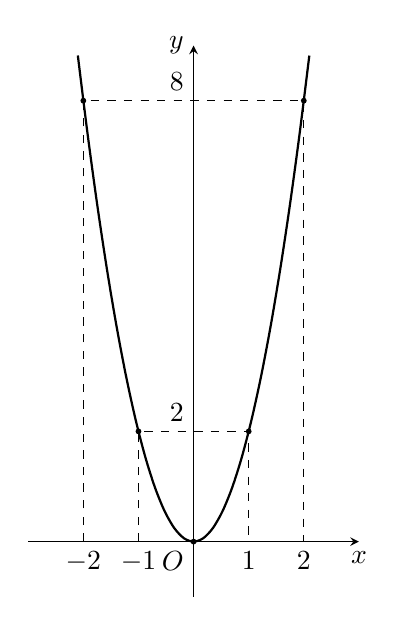
\begin{tikzpicture}[>=stealth, scale=0.7]
\draw[->] (-3,0) -- (3,0) node[below] {$x$};
\draw[->] (0,-1) -- (0,9) node[left] {$y$};
\fill (0,0) circle (1.5pt) node[below left] {$O$};
\draw[domain=-2.1:2.1, smooth, thick] plot (\x, {2*\x*\x});
\draw[dashed] (-2,0) node[below]{$-2$} |- (0,8) node[above left]{$8$} -| (2,0) node[below]{$2$};
\draw[dashed] (-1,0) node[below]{$-1$} |- (0,2) node[above left]{$2$} -| (1,0) node[below]{$1$};
\fill (-2,8) circle (1.5pt); \fill (2,8) circle (1.5pt);
\fill (-1,2) circle (1.5pt); \fill (1,2) circle (1.5pt);
\end{tikzpicture}
\end{center}
\textbf{b)} Tìm các điểm thuộc $(P)$ \hfill \textit{(0,5 điểm)} \par
Gọi điểm cần tìm là $C(x_C; y_C)$. Vì $C \in (P)$ và có tung độ $y_C = 18$ nên ta có phương trình:
$$ 2x_C^2 = 18 $$
$$ \Leftrightarrow x_C^2 = 9 $$
$$ \Leftrightarrow x_C = 3 \text{ hoặc } x_C = -3 $$
Với $x_C = 3$, ta được điểm $(3; 18)$. \par
Với $x_C = -3$, ta được điểm $(-3; 18)$. \par
Vậy tọa độ những điểm cần tìm là $(3; 18)$ và $(-3; 18)$[cite: 1, 12].
}
\end{bt}

\begin{bt}%[TS10 1.0 1.2]%[ma:49523185]
Cho parabol $(P): y = x^2$.
\textbf{a)} Vẽ đồ thị $(P)$ trên hệ trục tọa độ. \par
\textbf{b)} Tìm tọa độ những điểm thuộc $(P)$ có tung độ và hoành độ bằng nhau.
\loigiai{
\textbf{a)} Vẽ đồ thị $(P)$ \hfill \textit{(1,0 điểm)} \par
Bảng giá trị:
\begin{center}
\begin{tabular}{|c|c|c|c|c|c|}
\hline
$x$ & $-2$ & $-1$ & $0$ & $1$ & $2$ \\
\hline
$y = x^2$ & $4$ & $1$ & $0$ & $1$ & $4$ \\
\hline
\end{tabular}
\end{center}
Đồ thị hàm số $(P)$ là đường parabol đi qua gốc tọa độ $O$, nhận trục $Oy$ làm trục đối xứng và nằm phía trên trục hoành.
\begin{center}
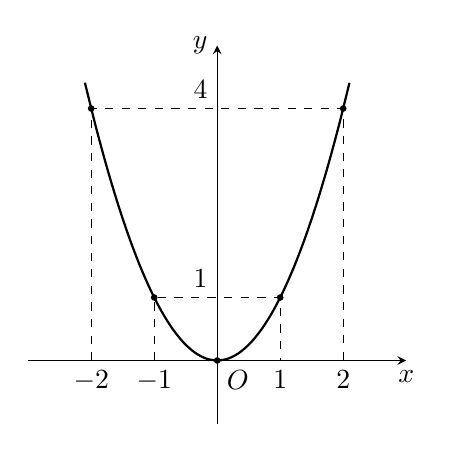
\begin{tikzpicture}[>=stealth, scale=0.8]
\draw[->] (-3,0) -- (3,0) node[below] {$x$};
\draw[->] (0,-1) -- (0,5) node[left] {$y$};
\fill (0,0) circle (1.5pt) node[below right] {$O$};
\draw[domain=-2.1:2.1, smooth, thick] plot (\x, {\x*\x});
\draw[dashed] (-2,0) node[below]{$-2$} |- (0,4) node[above left]{$4$} -| (2,0) node[below]{$2$};
\draw[dashed] (-1,0) node[below]{$-1$} |- (0,1) node[above left]{$1$} -| (1,0) node[below]{$1$};
\fill (-2,4) circle (1.5pt); \fill (2,4) circle (1.5pt);
\fill (-1,1) circle (1.5pt); \fill (1,1) circle (1.5pt);
\end{tikzpicture}
\end{center}
\textbf{b)} Tìm tọa độ các điểm \hfill \textit{(0,5 điểm)} \par
Gọi tọa độ điểm cần tìm là $D(x_D; y_D)$. Vì $D$ thuộc $(P)$ nên $y_D = x_D^2$. \par
Theo đề bài, tung độ và hoành độ bằng nhau nên $y_D = x_D$. \par
Ta có phương trình:
$$ x_D^2 = x_D $$
$$ \Leftrightarrow x_D^2 - x_D = 0 $$
$$ \Leftrightarrow x_D(x_D - 1) = 0 $$
$$ \Leftrightarrow \heva{&x_D = 0 \\ &x_D = 1} $$
Với $x_D = 0 \Rightarrow y_D = 0$, ta được điểm $D_1(0; 0)$[cite: 16]. \par
Với $x_D = 1 \Rightarrow y_D = 1$, ta được điểm $D_2(1; 1)$[cite: 16]. \par
Vậy tọa độ những điểm cần tìm là $(0; 0)$ và $(1; 1)$.
}
\end{bt}

\begin{bt}%[TS10 1.0 1.1]%[ma:414ff1a3]
Cho đồ thị hàm số $y = -\frac{1}{4}x^2$ có đồ thị là $(P)$.
\textbf{a)} Vẽ $(P)$ trên hệ trục tọa độ. \par
\textbf{b)} Tìm các điểm trên $(P)$ có tung độ bằng $-36$.
\loigiai{
\textbf{a)} Vẽ đồ thị $(P)$ \hfill \textit{(1,0 điểm)} \par
Bảng giá trị:
\begin{center}
\begin{tabular}{|c|c|c|c|c|c|}
\hline
$x$ & $-4$ & $-2$ & $0$ & $2$ & $4$ \\
\hline
$y = -\frac{1}{4}x^2$ & $-4$ & $-1$ & $0$ & $-1$ & $-4$ \\
\hline
\end{tabular}
\end{center}
Đồ thị hàm số $(P)$ là đường parabol đi qua gốc tọa độ $O$, nhận trục $Oy$ làm trục đối xứng và nằm phía dưới trục hoành.
\begin{center}
\begin{tikzpicture}[>=stealth, scale=0.8]
\draw[->] (-5,0) -- (5,0) node[above] {$x$};
\draw[->] (0,-5) -- (0,1) node[right] {$y$};
\fill (0,0) circle (1.5pt) node[above right] {$O$};
\draw[domain=-4.2:4.2, smooth, thick] plot (\x, {-0.25*\x*\x});
\draw[dashed] (-4,0) node[above]{$-4$} |- (0,-4) node[below left]{$-4$} -| (4,0) node[above]{$4$};
\draw[dashed] (-2,0) node[above]{$-2$} |- (0,-1) node[below left]{$-1$} -| (2,0) node[above]{$2$};
\fill (-4,-4) circle (1.5pt); \fill (4,-4) circle (1.5pt);
\fill (-2,-1) circle (1.5pt); \fill (2,-1) circle (1.5pt);
\end{tikzpicture}
\end{center}
\textbf{b)} Tìm các điểm trên $(P)$ \hfill \textit{(0,5 điểm)} \par
Gọi điểm cần tìm là $E(x_E; y_E)$. Vì $E \in (P)$ và có tung độ $y_E = -36$ nên ta có phương trình:
$$ -\frac{1}{4}x_E^2 = -36 $$
$$ \Leftrightarrow x_E^2 = 144 $$
$$ \Leftrightarrow x_E = 12 \text{ hoặc } x_E = -12 $$
Với $x_E = 12$, ta có điểm $E_1(12; -36)$[cite: 47]. \par
Với $x_E = -12$, ta có điểm $E_2(-12; -36)$[cite: 47]. \par
Vậy có hai điểm trên $(P)$ thỏa mãn yêu cầu là $(12; -36)$ và $(-12; -36)$.
}
\end{bt}

\begin{bt}%[TS10 1.0 1.2]%[ma:8e4727d0]
Cho parabol $(P): y = \frac{x^2}{4}$.
\textbf{a)} Vẽ đồ thị $(P)$ của hàm số trên. \par
\textbf{b)} Tìm những điểm thuộc $(P)$ sao cho tung độ gấp $4$ lần hoành độ.
\loigiai{
\textbf{a)} Vẽ đồ thị $(P)$ \hfill \textit{(1,0 điểm)} \par
Bảng giá trị:
\begin{center}
\begin{tabular}{|c|c|c|c|c|c|}
\hline
$x$ & $-4$ & $-2$ & $0$ & $2$ & $4$ \\
\hline
$y = \frac{x^2}{4}$ & $4$ & $1$ & $0$ & $1$ & $4$ \\
\hline
\end{tabular}
\end{center}
Đồ thị hàm số $(P)$ là đường parabol đi qua gốc tọa độ $O$, nhận trục $Oy$ làm trục đối xứng và nằm phía trên trục hoành.
\begin{center}
\begin{tikzpicture}[>=stealth, scale=0.8]
\draw[->] (-5,0) -- (5,0) node[below] {$x$};
\draw[->] (0,-1) -- (0,5) node[left] {$y$};
\fill (0,0) circle (1.5pt) node[below left] {$O$};
\draw[domain=-4.2:4.2, smooth, thick] plot (\x, {0.25*\x*\x});
\draw[dashed] (-4,0) node[below]{$-4$} |- (0,4) node[above left]{$4$} -| (4,0) node[below]{$4$};
\draw[dashed] (-2,0) node[below]{$-2$} |- (0,1) node[above left]{$1$} -| (2,0) node[below]{$2$};
\fill (-4,4) circle (1.5pt); \fill (4,4) circle (1.5pt);
\fill (-2,1) circle (1.5pt); \fill (2,1) circle (1.5pt);
\end{tikzpicture}
\end{center}
\textbf{b)} Tìm những điểm thuộc $(P)$ \hfill \textit{(0,5 điểm)} \par
Gọi điểm cần tìm là $F(x_F; y_F)$. Vì $F \in (P)$ nên $y_F = \frac{1}{4}x_F^2$. \par
Theo đề bài, tung độ gấp $4$ lần hoành độ nên $y_F = 4x_F$[cite: 1, 24]. \par
Ta có phương trình:
$$ \frac{1}{4}x_F^2 = 4x_F $$
$$ \Leftrightarrow x_F^2 - 16x_F = 0 $$
$$ \Leftrightarrow x_F(x_F - 16) = 0 $$
$$ \Leftrightarrow \heva{&x_F = 0 \\ &x_F = 16} $$
Với $x_F = 0 \Rightarrow y_F = 0$, ta được điểm $F_1(0; 0)$. \par
Với $x_F = 16 \Rightarrow y_F = 4(16) = 64$, ta được điểm $F_2(16; 64)$. \par
Vậy tọa độ những điểm cần tìm là $(0; 0)$ và $(16; 64)$.
}
\end{bt}

\begin{bt}%[TS10 1.0 1.1]%[ma:6020ba7e]
Cho hàm số $y = -\frac{x^2}{2}$ có đồ thị là $(P)$.
\textbf{a)} Vẽ đồ thị $(P)$ trên hệ trục tọa độ. \par
\textbf{b)} Tìm tọa độ điểm $A$ thuộc $(P)$ có tung độ bằng $-2$.
\loigiai{
\textbf{a)} Vẽ đồ thị $(P)$ \hfill \textit{(1,0 điểm)} \par
Bảng giá trị:
\begin{center}
\begin{tabular}{|c|c|c|c|c|c|}
\hline
$x$ & $-4$ & $-2$ & $0$ & $2$ & $4$ \\
\hline
$y = -\frac{x^2}{2}$ & $-8$ & $-2$ & $0$ & $-2$ & $-8$ \\
\hline
\end{tabular}
\end{center}
Đồ thị hàm số $(P)$ là đường parabol đi qua gốc tọa độ $O$, nhận trục $Oy$ làm trục đối xứng và nằm phía dưới trục hoành.
\begin{center}
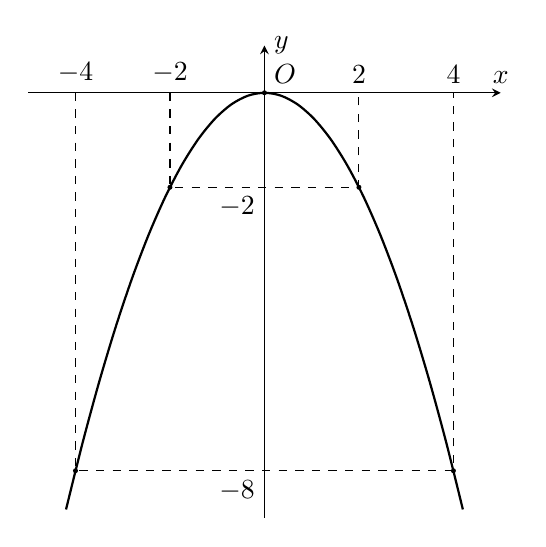
\begin{tikzpicture}[>=stealth, scale=0.6]
\draw[->] (-5,0) -- (5,0) node[above] {$x$};
\draw[->] (0,-9) -- (0,1) node[right] {$y$};
\fill (0,0) circle (1.5pt) node[above right] {$O$};
\draw[domain=-4.2:4.2, smooth, thick] plot (\x, {-0.5*\x*\x});
\draw[dashed] (-4,0) node[above]{$-4$} |- (0,-8) node[below left]{$-8$} -| (4,0) node[above]{$4$};
\draw[dashed] (-2,0) node[above]{$-2$} |- (0,-2) node[below left]{$-2$} -| (2,0) node[above]{$2$};
\fill (-4,-8) circle (1.5pt); \fill (4,-8) circle (1.5pt);
\fill (-2,-2) circle (1.5pt); \fill (2,-2) circle (1.5pt);
\end{tikzpicture}
\end{center}
\textbf{b)} Tìm tọa độ điểm $A$ \hfill \textit{(0,5 điểm)} \par
Vì điểm $A$ thuộc $(P)$ và có tung độ bằng $-2$ nên ta thay $y = -2$ vào phương trình hàm số:
$$ -2 = -\frac{x^2}{2} $$
$$ \Leftrightarrow x^2 = 4 $$
$$ \Leftrightarrow x = 2 \text{ hoặc } x = -2 $$
Với $x = 2$, ta được điểm $(2; -2)$. \par
Với $x = -2$, ta được điểm $(-2; -2)$. \par
Vậy tọa độ các điểm $A$ cần tìm là $(2; -2)$ và $(-2; -2)$[cite: 1].
}
\end{bt}

\begin{bt}%[TS10 1.0 1.2]%[ma:43206e52]
Cho hàm số $y = 2x^2$ có đồ thị là parabol $(P)$.
\textbf{a)} Vẽ $(P)$ trên hệ trục tọa độ. \par
\textbf{b)} Tìm tọa độ các điểm $K$ thuộc $(P)$ có hoành độ bằng hai lần tung độ.
\loigiai{
\textbf{a)} Vẽ đồ thị $(P)$ \hfill \textit{(1,0 điểm)} \par
Bảng giá trị:
\begin{center}
\begin{tabular}{|c|c|c|c|c|c|}
\hline
$x$ & $-2$ & $-1$ & $0$ & $1$ & $2$ \\
\hline
$y = 2x^2$ & $8$ & $2$ & $0$ & $2$ & $8$ \\
\hline
\end{tabular}
\end{center}
Đồ thị hàm số $(P)$ là đường parabol đi qua gốc tọa độ $O$, nhận trục $Oy$ làm trục đối xứng và nằm phía trên trục hoành.
\begin{center}
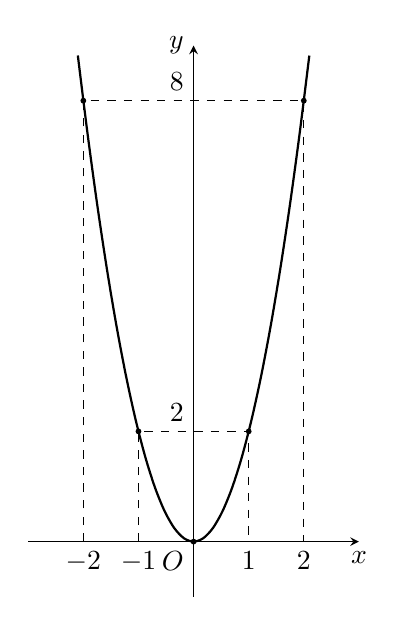
\begin{tikzpicture}[>=stealth, scale=0.7]
\draw[->] (-3,0) -- (3,0) node[below] {$x$};
\draw[->] (0,-1) -- (0,9) node[left] {$y$};
\fill (0,0) circle (1.5pt) node[below left] {$O$};
\draw[domain=-2.1:2.1, smooth, thick] plot (\x, {2*\x*\x});
\draw[dashed] (-2,0) node[below]{$-2$} |- (0,8) node[above left]{$8$} -| (2,0) node[below]{$2$};
\draw[dashed] (-1,0) node[below]{$-1$} |- (0,2) node[above left]{$2$} -| (1,0) node[below]{$1$};
\fill (-2,8) circle (1.5pt); \fill (2,8) circle (1.5pt);
\fill (-1,2) circle (1.5pt); \fill (1,2) circle (1.5pt);
\end{tikzpicture}
\end{center}
\textbf{b)} Tìm tọa độ các điểm $K$ \hfill \textit{(0,5 điểm)} \par
Gọi tọa độ điểm $K$ là $(x_K; y_K)$. Vì $K \in (P)$ nên $y_K = 2x_K^2$. \par
Theo đề bài, hoành độ bằng hai lần tung độ nên $x_K = 2y_K$[cite: 36]. \par
Ta có phương trình:
$$ x_K = 2(2x_K^2) $$
$$ \Leftrightarrow 4x_K^2 - x_K = 0 $$
$$ \Leftrightarrow x_K(4x_K - 1) = 0 $$
$$ \Leftrightarrow \heva{&x_K = 0 \\ &x_K = \frac{1}{4}} $$
Với $x_K = 0 \Rightarrow y_K = 0$, ta được điểm $K_1(0; 0)$[cite: 36]. \par
Với $x_K = \frac{1}{4} \Rightarrow y_K = 2\left(\frac{1}{4}\right)^2 = 2 \cdot \frac{1}{16} = \frac{1}{8}$. \par
(Kiểm tra lại: $x_K = 2y_K \Leftrightarrow \frac{1}{4} = 2 \cdot \frac{1}{8}$ đúng). \par
Ta được điểm $K_2\left(\frac{1}{4}; \frac{1}{8}\right)$. \par
Vậy tọa độ các điểm cần tìm là $(0; 0)$ và $\left(\frac{1}{4}; \frac{1}{8}\right)$[cite: 36].
}
\end{bt}


\begin{bt}%[TS10 1.0 1.3]%[ma:4db76812]
Cho parabol $(P): y = x^2$.
\textbf{a)} Vẽ đồ thị $(P)$ trên mặt phẳng tọa độ. \par
\textbf{b)} Tìm tọa độ các điểm $A$ thuộc $(P)$ sao cho tổng hoành độ và tung độ của điểm đó bằng $6$.
\loigiai{
\textbf{a)} Vẽ đồ thị $(P): y = x^2$ \hfill \textit{(1,0 điểm)} \par
Bảng giá trị:
\begin{center}
\begin{tabular}{|c|c|c|c|c|c|}
\hline
$x$ & $-2$ & $-1$ & $0$ & $1$ & $2$ \\
\hline
$y = x^2$ & $4$ & $1$ & $0$ & $1$ & $4$ \\
\hline
\end{tabular}
\end{center}
Đồ thị hàm số $(P)$ là một đường parabol đi qua gốc tọa độ $O$, nhận trục $Oy$ làm trục đối xứng và nằm phía trên trục hoành.
\begin{center}
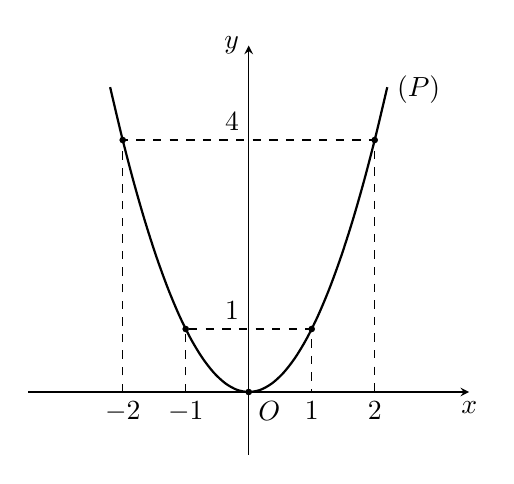
\begin{tikzpicture}[>=stealth, scale=0.8]
\draw[->] (-3.5,0) -- (3.5,0) node[below] {$x$};
\draw[->] (0,-1) -- (0,5.5) node[left] {$y$};
\fill (0,0) circle (1.5pt) node[below right] {$O$};
\draw[domain=-2.2:2.2, smooth, thick] plot (\x, {\x*\x});
\draw[dashed] (-2,0) node[below]{$-2$} |- (0,4) node[above left]{$4$} -| (2,0) node[below]{$2$};
\draw[dashed] (-1,0) node[below]{$-1$} |- (0,1) node[above left]{$1$} -| (1,0) node[below]{$1$};
\fill (-2,4) circle (1.5pt); \fill (2,4) circle (1.5pt);
\fill (-1,1) circle (1.5pt); \fill (1,1) circle (1.5pt);
\node[right] at (2.2, 4.8) {$(P)$};
\end{tikzpicture}
\end{center}
\textbf{b)} Tìm tọa độ các điểm $A$ \hfill \textit{(0,5 điểm)} \par
Gọi tọa độ điểm $A$ là $(x_A; y_A)$. Vì $A \in (P)$ nên $y_A = x_A^2$. \par
Theo đề bài, tổng hoành độ và tung độ bằng $6$, ta có phương trình:
$$ x_A + y_A = 6 $$
$$ \Leftrightarrow x_A + x_A^2 = 6 $$
$$ \Leftrightarrow x_A^2 + x_A - 6 = 0 $$
$$ \Leftrightarrow (x_A - 2)(x_A + 3) = 0 $$
$$ \Leftrightarrow \heva{&x_A = 2 \\ &x_A = -3} $$
Với $x_A = 2 \Rightarrow y_A = 2^2 = 4$, ta được điểm $A_1(2; 4)$. \par
Với $x_A = -3 \Rightarrow y_A = (-3)^2 = 9$, ta được điểm $A_2(-3; 9)$. \par
Vậy tọa độ các điểm $A$ cần tìm là $(2; 4)$ và $(-3; 9)$.
}
\end{bt}

\begin{bt}%[TS10 1.0 1.4]%[ma:c8ebd171]
Cho parabol $(P): y = -x^2$ và đường thẳng $(d): y = 3x - 4$.
\textbf{a)} Vẽ đồ thị $(P)$ trên hệ trục tọa độ. \par
\textbf{b)} Tìm tọa độ giao điểm của $(P)$ và $(d)$ bằng phép tính.
\loigiai{
\textbf{a)} Vẽ đồ thị $(P): y = -x^2$ \hfill \textit{(1,0 điểm)} \par
Bảng giá trị:
\begin{center}
\begin{tabular}{|c|c|c|c|c|c|}
\hline
$x$ & $-2$ & $-1$ & $0$ & $1$ & $2$ \\
\hline
$y = -x^2$ & $-4$ & $-1$ & $0$ & $-1$ & $-4$ \\
\hline
\end{tabular}
\end{center}
Đồ thị hàm số $(P)$ là một đường parabol đi qua gốc tọa độ $O$, nhận trục $Oy$ làm trục đối xứng và nằm phía dưới trục hoành.
\begin{center}
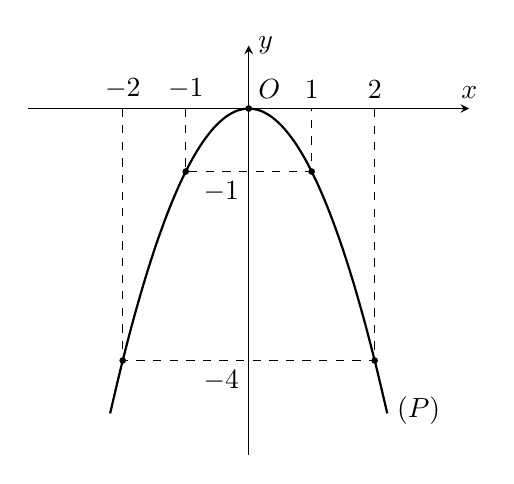
\begin{tikzpicture}[>=stealth, scale=0.8]
\draw[->] (-3.5,0) -- (3.5,0) node[above] {$x$};
\draw[->] (0,-5.5) -- (0,1) node[right] {$y$};
\fill (0,0) circle (1.5pt) node[above right] {$O$};
\draw[domain=-2.2:2.2, smooth, thick] plot (\x, {-\x*\x});
\draw[dashed] (-2,0) node[above]{$-2$} |- (0,-4) node[below left]{$-4$} -| (2,0) node[above]{$2$};
\draw[dashed] (-1,0) node[above]{$-1$} |- (0,-1) node[below left]{$-1$} -| (1,0) node[above]{$1$};
\fill (-2,-4) circle (1.5pt); \fill (2,-4) circle (1.5pt);
\fill (-1,-1) circle (1.5pt); \fill (1,-1) circle (1.5pt);
\node[right] at (2.2, -4.8) {$(P)$};
\end{tikzpicture}
\end{center}
\textbf{b)} Tìm tọa độ giao điểm của $(P)$ và $(d)$ \hfill \textit{(0,5 điểm)} \par
Phương trình hoành độ giao điểm của $(P)$ và $(d)$ là:
$$ -x^2 = 3x - 4 $$
$$ \Leftrightarrow x^2 + 3x - 4 = 0 $$
Vì $a + b + c = 1 + 3 + (-4) = 0$ nên phương trình có hai nghiệm:
$$ x_1 = 1; \quad x_2 = -4 $$
Với $x = 1 \Rightarrow y = -(1)^2 = -1$. Ta được giao điểm thứ nhất là $(1; -1)$. \par
Với $x = -4 \Rightarrow y = -(-4)^2 = -16$. Ta được giao điểm thứ hai là $(-4; -16)$. \par
Vậy tọa độ giao điểm của $(P)$ và $(d)$ là $(1; -1)$ và $(-4; -16)$.
}
\end{bt}

\begin{bt}%[TS10 1.0 1.3]%[ma:9fb93691]
Cho parabol $(P): y = \frac{1}{2}x^2$.
\textbf{a)} Vẽ đồ thị $(P)$ trên hệ trục tọa độ. \par
\textbf{b)} Tìm tọa độ các điểm $B$ thuộc $(P)$ sao cho tung độ lớn hơn hoành độ $4$ đơn vị.
\loigiai{
\textbf{a)} Vẽ đồ thị $(P): y = \frac{1}{2}x^2$ \hfill \textit{(1,0 điểm)} \par
Bảng giá trị:
\begin{center}
\begin{tabular}{|c|c|c|c|c|c|}
\hline
$x$ & $-4$ & $-2$ & $0$ & $2$ & $4$ \\
\hline
$y = \frac{1}{2}x^2$ & $8$ & $2$ & $0$ & $2$ & $8$ \\
\hline
\end{tabular}
\end{center}
Đồ thị hàm số $(P)$ là một đường parabol đi qua gốc tọa độ $O$, nhận trục $Oy$ làm trục đối xứng và nằm phía trên trục hoành.
\begin{center}
\begin{tikzpicture}[>=stealth, scale=0.7]
\draw[->] (-5.5,0) -- (5.5,0) node[below] {$x$};
\draw[->] (0,-1) -- (0,9.5) node[left] {$y$};
\fill (0,0) circle (1.5pt) node[below right] {$O$};
\draw[domain=-4.2:4.2, smooth, thick] plot (\x, {0.5*\x*\x});
\draw[dashed] (-4,0) node[below]{$-4$} |- (0,8) node[above left]{$8$} -| (4,0) node[below]{$4$};
\draw[dashed] (-2,0) node[below]{$-2$} |- (0,2) node[above left]{$2$} -| (2,0) node[below]{$2$};
\fill (-4,8) circle (1.5pt); \fill (4,8) circle (1.5pt);
\fill (-2,2) circle (1.5pt); \fill (2,2) circle (1.5pt);
\node[right] at (4.2, 8.8) {$(P)$};
\end{tikzpicture}
\end{center}
\textbf{b)} Tìm tọa độ các điểm $B$ \hfill \textit{(0,5 điểm)} \par
Gọi tọa độ điểm $B$ là $(x_B; y_B)$. Vì $B \in (P)$ nên $y_B = \frac{1}{2}x_B^2$. \par
Theo đề bài, tung độ lớn hơn hoành độ $4$ đơn vị, ta có phương trình:
$$ y_B - x_B = 4 $$
$$ \Leftrightarrow \frac{1}{2}x_B^2 - x_B - 4 = 0 $$
$$ \Leftrightarrow x_B^2 - 2x_B - 8 = 0 $$
$$ \Leftrightarrow (x_B - 4)(x_B + 2) = 0 $$
$$ \Leftrightarrow \heva{&x_B = 4 \\ &x_B = -2} $$
Với $x_B = 4 \Rightarrow y_B = \frac{1}{2} \cdot 4^2 = 8$, ta được điểm $B_1(4; 8)$. \par
Với $x_B = -2 \Rightarrow y_B = \frac{1}{2} \cdot (-2)^2 = 2$, ta được điểm $B_2(-2; 2)$. \par
Vậy tọa độ các điểm $B$ cần tìm là $(4; 8)$ và $(-2; 2)$.
}
\end{bt}

\begin{bt}%[TS10 1.0 1.4]%[ma:a40b5424]
Cho parabol $(P): y = -\frac{1}{4}x^2$ và đường thẳng $(d): y = \frac{1}{2}x - 2$.
\textbf{a)} Vẽ đồ thị $(P)$ trên hệ trục tọa độ. \par
\textbf{b)} Bằng phép tính, tìm tọa độ giao điểm của $(P)$ và $(d)$.
\loigiai{
\textbf{a)} Vẽ đồ thị $(P): y = -\frac{1}{4}x^2$ \hfill \textit{(1,0 điểm)} \par
Bảng giá trị:
\begin{center}
\begin{tabular}{|c|c|c|c|c|c|}
\hline
$x$ & $-4$ & $-2$ & $0$ & $2$ & $4$ \\
\hline
$y = -\frac{1}{4}x^2$ & $-4$ & $-1$ & $0$ & $-1$ & $-4$ \\
\hline
\end{tabular}
\end{center}
Đồ thị hàm số $(P)$ là một đường parabol đi qua gốc tọa độ $O$, nhận trục $Oy$ làm trục đối xứng và nằm phía dưới trục hoành.
\begin{center}
\begin{tikzpicture}[>=stealth, scale=0.8]
\draw[->] (-5.5,0) -- (5.5,0) node[above] {$x$};
\draw[->] (0,-5.5) -- (0,1) node[right] {$y$};
\fill (0,0) circle (1.5pt) node[above right] {$O$};
\draw[domain=-4.5:4.5, smooth, thick] plot (\x, {-0.25*\x*\x});
\draw[dashed] (-4,0) node[above]{$-4$} |- (0,-4) node[below left]{$-4$} -| (4,0) node[above]{$4$};
\draw[dashed] (-2,0) node[above]{$-2$} |- (0,-1) node[below left]{$-1$} -| (2,0) node[above]{$2$};
\fill (-4,-4) circle (1.5pt); \fill (4,-4) circle (1.5pt);
\fill (-2,-1) circle (1.5pt); \fill (2,-1) circle (1.5pt);
\node[right] at (4.5, -5) {$(P)$};
\end{tikzpicture}
\end{center}
\textbf{b)} Tìm tọa độ giao điểm của $(P)$ và $(d)$ \hfill \textit{(0,5 điểm)} \par
Phương trình hoành độ giao điểm của $(P)$ và $(d)$ là:
$$ -\frac{1}{4}x^2 = \frac{1}{2}x - 2 $$
$$ \Leftrightarrow x^2 + 2x - 8 = 0 $$
$$ \Leftrightarrow (x - 2)(x + 4) = 0 $$
$$ \Leftrightarrow \heva{&x = 2 \\ &x = -4} $$
Với $x = 2 \Rightarrow y = -\frac{1}{4}(2)^2 = -1$. Ta được giao điểm thứ nhất là $(2; -1)$. \par
Với $x = -4 \Rightarrow y = -\frac{1}{4}(-4)^2 = -4$. Ta được giao điểm thứ hai là $(-4; -4)$. \par
Vậy tọa độ giao điểm của $(P)$ và $(d)$ là $(2; -1)$ và $(-4; -4)$.
}
\end{bt}

\begin{bt}%[TS10 1.0 1.3]%[ma:907b5db8]
Cho parabol $(P): y = \frac{1}{4}x^2$.
\textbf{a)} Vẽ đồ thị $(P)$ trên mặt phẳng tọa độ. \par
\textbf{b)} Tìm tọa độ các điểm $C$ thuộc $(P)$ (khác gốc tọa độ $O$) sao cho tích của hoành độ và tung độ bằng $2$.
\loigiai{
\textbf{a)} Vẽ đồ thị $(P): y = \frac{1}{4}x^2$ \hfill \textit{(1,0 điểm)} \par
Bảng giá trị:
\begin{center}
\begin{tabular}{|c|c|c|c|c|c|}
\hline
$x$ & $-4$ & $-2$ & $0$ & $2$ & $4$ \\
\hline
$y = \frac{1}{4}x^2$ & $4$ & $1$ & $0$ & $1$ & $4$ \\
\hline
\end{tabular}
\end{center}
Đồ thị hàm số $(P)$ là một đường parabol đi qua gốc tọa độ $O$, nhận trục $Oy$ làm trục đối xứng và nằm phía trên trục hoành.
\begin{center}
\begin{tikzpicture}[>=stealth, scale=0.8]
\draw[->] (-5.5,0) -- (5.5,0) node[below] {$x$};
\draw[->] (0,-1) -- (0,5.5) node[left] {$y$};
\fill (0,0) circle (1.5pt) node[below right] {$O$};
\draw[domain=-4.2:4.2, smooth, thick] plot (\x, {0.25*\x*\x});
\draw[dashed] (-4,0) node[below]{$-4$} |- (0,4) node[above left]{$4$} -| (4,0) node[below]{$4$};
\draw[dashed] (-2,0) node[below]{$-2$} |- (0,1) node[above left]{$1$} -| (2,0) node[below]{$2$};
\fill (-4,4) circle (1.5pt); \fill (4,4) circle (1.5pt);
\fill (-2,1) circle (1.5pt); \fill (2,1) circle (1.5pt);
\node[right] at (4.2, 4.4) {$(P)$};
\end{tikzpicture}
\end{center}
\textbf{b)} Tìm tọa độ các điểm $C$ \hfill \textit{(0,5 điểm)} \par
Gọi tọa độ điểm $C$ là $(x_C; y_C)$. Vì $C \in (P)$ nên $y_C = \frac{1}{4}x_C^2$. \par
Theo đề bài, tích của hoành độ và tung độ bằng $2$, ta có phương trình:
$$ x_C \cdot y_C = 2 $$
$$ \Leftrightarrow x_C \cdot \left(\frac{1}{4}x_C^2\right) = 2 $$
$$ \Leftrightarrow x_C^3 = 8 $$
$$ \Leftrightarrow x_C = 2 $$
Với $x_C = 2 \Rightarrow y_C = \frac{1}{4} \cdot 2^2 = 1$. Ta được điểm $C(2; 1)$. \par
Vậy tọa độ điểm $C$ cần tìm là $(2; 1)$.
}
\end{bt}

\begin{bt}%[TS10 1.0 1.4]%[ma:887c2273]
Cho parabol $(P): y = \frac{1}{2}x^2$ và đường thẳng $(d): y = -x + 4$.
\textbf{a)} Vẽ đồ thị $(P)$ trên hệ trục tọa độ. \par
\textbf{b)} Tìm tọa độ giao điểm của $(P)$ và $(d)$ bằng phép tính.
\loigiai{
\textbf{a)} Vẽ đồ thị $(P): y = \frac{1}{2}x^2$ \hfill \textit{(1,0 điểm)} \par
Bảng giá trị:
\begin{center}
\begin{tabular}{|c|c|c|c|c|c|}
\hline
$x$ & $-4$ & $-2$ & $0$ & $2$ & $4$ \\
\hline
$y = \frac{1}{2}x^2$ & $8$ & $2$ & $0$ & $2$ & $8$ \\
\hline
\end{tabular}
\end{center}
Đồ thị hàm số $(P)$ là một đường parabol đi qua gốc tọa độ $O$, nhận trục $Oy$ làm trục đối xứng và nằm phía trên trục hoành.
\begin{center}
\begin{tikzpicture}[>=stealth, scale=0.7]
\draw[->] (-5.5,0) -- (5.5,0) node[below] {$x$};
\draw[->] (0,-1) -- (0,9.5) node[left] {$y$};
\fill (0,0) circle (1.5pt) node[below right] {$O$};
\draw[domain=-4.2:4.2, smooth, thick] plot (\x, {0.5*\x*\x});
\draw[dashed] (-4,0) node[below]{$-4$} |- (0,8) node[above left]{$8$} -| (4,0) node[below]{$4$};
\draw[dashed] (-2,0) node[below]{$-2$} |- (0,2) node[above left]{$2$} -| (2,0) node[below]{$2$};
\fill (-4,8) circle (1.5pt); \fill (4,8) circle (1.5pt);
\fill (-2,2) circle (1.5pt); \fill (2,2) circle (1.5pt);
\node[right] at (4.2, 8.8) {$(P)$};
\end{tikzpicture}
\end{center}
\textbf{b)} Tìm tọa độ giao điểm của $(P)$ và $(d)$ \hfill \textit{(0,5 điểm)} \par
Phương trình hoành độ giao điểm của $(P)$ và $(d)$ là:
$$ \frac{1}{2}x^2 = -x + 4 $$
$$ \Leftrightarrow x^2 + 2x - 8 = 0 $$
$$ \Leftrightarrow (x - 2)(x + 4) = 0 $$
$$ \Leftrightarrow \heva{&x = 2 \\ &x = -4} $$
Với $x = 2 \Rightarrow y = -2 + 4 = 2$. Ta được giao điểm thứ nhất là $(2; 2)$. \par
Với $x = -4 \Rightarrow y = -(-4) + 4 = 8$. Ta được giao điểm thứ hai là $(-4; 8)$. \par
Vậy tọa độ giao điểm của $(P)$ và $(d)$ là $(2; 2)$ và $(-4; 8)$.
}
\end{bt}

\begin{bt}%[TS10 1.0 1.3]%[ma:2e1a2858]
Cho parabol $(P): y = -x^2$.
\textbf{a)} Vẽ đồ thị $(P)$ trên mặt phẳng tọa độ $Oxy$. \par
\textbf{b)} Tìm tọa độ các điểm $M$ thuộc $(P)$ sao cho hiệu của hoành độ và tung độ bằng $2$.
\loigiai{
\textbf{a)} Vẽ đồ thị $(P): y = -x^2$ \hfill \textit{(1,0 điểm)} \par
Bảng giá trị:
\begin{center}
\begin{tabular}{|c|c|c|c|c|c|}
\hline
$x$ & $-2$ & $-1$ & $0$ & $1$ & $2$ \\
\hline
$y = -x^2$ & $-4$ & $-1$ & $0$ & $-1$ & $-4$ \\
\hline
\end{tabular}
\end{center}
Đồ thị hàm số $(P)$ là một đường parabol đi qua gốc tọa độ $O$, nhận trục $Oy$ làm trục đối xứng và nằm phía dưới trục hoành.
\begin{center}
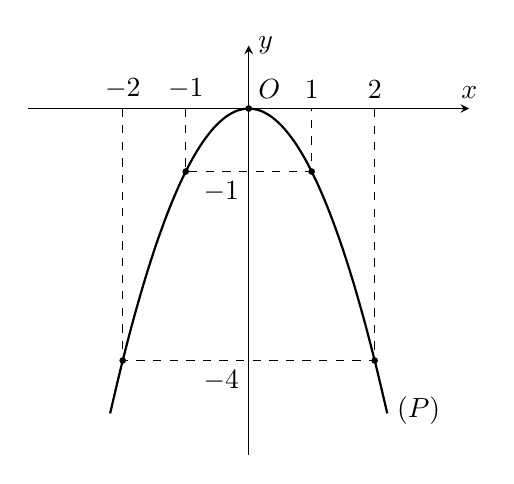
\begin{tikzpicture}[>=stealth, scale=0.8]
\draw[->] (-3.5,0) -- (3.5,0) node[above] {$x$};
\draw[->] (0,-5.5) -- (0,1) node[right] {$y$};
\fill (0,0) circle (1.5pt) node[above right] {$O$};
\draw[domain=-2.2:2.2, smooth, thick] plot (\x, {-\x*\x});
\draw[dashed] (-2,0) node[above]{$-2$} |- (0,-4) node[below left]{$-4$} -| (2,0) node[above]{$2$};
\draw[dashed] (-1,0) node[above]{$-1$} |- (0,-1) node[below left]{$-1$} -| (1,0) node[above]{$1$};
\fill (-2,-4) circle (1.5pt); \fill (2,-4) circle (1.5pt);
\fill (-1,-1) circle (1.5pt); \fill (1,-1) circle (1.5pt);
\node[right] at (2.2, -4.8) {$(P)$};
\end{tikzpicture}
\end{center}
\textbf{b)} Tìm tọa độ các điểm $M$ \hfill \textit{(0,5 điểm)} \par
Gọi tọa độ điểm $M$ là $(x_M; y_M)$. Vì $M \in (P)$ nên $y_M = -x_M^2$. \par
Theo đề bài, hiệu của hoành độ và tung độ bằng $2$, ta có phương trình:
$$ x_M - y_M = 2 $$
$$ \Leftrightarrow x_M - (-x_M^2) = 2 $$
$$ \Leftrightarrow x_M^2 + x_M - 2 = 0 $$
Vì $a + b + c = 1 + 1 + (-2) = 0$ nên phương trình có hai nghiệm:
$$ x_{M1} = 1; \quad x_{M2} = -2 $$
Với $x_M = 1 \Rightarrow y_M = -(1)^2 = -1$, ta được điểm $M_1(1; -1)$. \par
Với $x_M = -2 \Rightarrow y_M = -(-2)^2 = -4$, ta được điểm $M_2(-2; -4)$. \par
Vậy tọa độ các điểm $M$ cần tìm là $(1; -1)$ và $(-2; -4)$.
}
\end{bt}

\begin{bt}%[TS10 1.0 1.4]%[ma:3f40a071]
Cho parabol $(P): y = x^2$ và đường thẳng $(d): y = -2x + 3$.
\textbf{a)} Vẽ đồ thị $(P)$ trên hệ trục tọa độ. \par
\textbf{b)} Tìm tọa độ giao điểm của $(P)$ và $(d)$ bằng phép tính.
\loigiai{
\textbf{a)} Vẽ đồ thị $(P): y = x^2$ \hfill \textit{(1,0 điểm)} \par
Bảng giá trị:
\begin{center}
\begin{tabular}{|c|c|c|c|c|c|}
\hline
$x$ & $-2$ & $-1$ & $0$ & $1$ & $2$ \\
\hline
$y = x^2$ & $4$ & $1$ & $0$ & $1$ & $4$ \\
\hline
\end{tabular}
\end{center}
Đồ thị hàm số $(P)$ là một đường parabol đi qua gốc tọa độ $O$, nhận trục $Oy$ làm trục đối xứng và nằm phía trên trục hoành.
\begin{center}
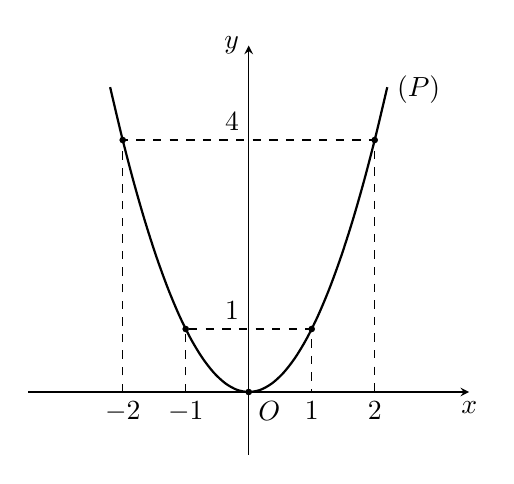
\begin{tikzpicture}[>=stealth, scale=0.8]
\draw[->] (-3.5,0) -- (3.5,0) node[below] {$x$};
\draw[->] (0,-1) -- (0,5.5) node[left] {$y$};
\fill (0,0) circle (1.5pt) node[below right] {$O$};
\draw[domain=-2.2:2.2, smooth, thick] plot (\x, {\x*\x});
\draw[dashed] (-2,0) node[below]{$-2$} |- (0,4) node[above left]{$4$} -| (2,0) node[below]{$2$};
\draw[dashed] (-1,0) node[below]{$-1$} |- (0,1) node[above left]{$1$} -| (1,0) node[below]{$1$};
\fill (-2,4) circle (1.5pt); \fill (2,4) circle (1.5pt);
\fill (-1,1) circle (1.5pt); \fill (1,1) circle (1.5pt);
\node[right] at (2.2, 4.8) {$(P)$};
\end{tikzpicture}
\end{center}
\textbf{b)} Tìm tọa độ giao điểm của $(P)$ và $(d)$ \hfill \textit{(0,5 điểm)} \par
Phương trình hoành độ giao điểm của $(P)$ và $(d)$ là:
$$ x^2 = -2x + 3 $$
$$ \Leftrightarrow x^2 + 2x - 3 = 0 $$
Vì $a + b + c = 1 + 2 + (-3) = 0$ nên phương trình có hai nghiệm:
$$ x_1 = 1; \quad x_2 = -3 $$
Với $x = 1 \Rightarrow y = (1)^2 = 1$. Ta được giao điểm thứ nhất là $(1; 1)$. \par
Với $x = -3 \Rightarrow y = (-3)^2 = 9$. Ta được giao điểm thứ hai là $(-3; 9)$. \par
Vậy tọa độ giao điểm của $(P)$ và $(d)$ là $(1; 1)$ và $(-3; 9)$.
}
\end{bt}

\begin{bt}%[TS10 1.0 1.3]%[ma:713c727b]
Cho parabol $(P): y = 2x^2$.
\textbf{a)} Vẽ đồ thị $(P)$ trên hệ trục tọa độ. \par
\textbf{b)} Tìm tọa độ các điểm $E$ thuộc $(P)$ sao cho tổng hoành độ và tung độ của điểm đó bằng $3$.
\loigiai{
\textbf{a)} Vẽ đồ thị $(P): y = 2x^2$ \hfill \textit{(1,0 điểm)} \par
Bảng giá trị:
\begin{center}
\begin{tabular}{|c|c|c|c|c|c|}
\hline
$x$ & $-2$ & $-1$ & $0$ & $1$ & $2$ \\
\hline
$y = 2x^2$ & $8$ & $2$ & $0$ & $2$ & $8$ \\
\hline
\end{tabular}
\end{center}
Đồ thị hàm số $(P)$ là một đường parabol đi qua gốc tọa độ $O$, nhận trục $Oy$ làm trục đối xứng và nằm phía trên trục hoành.
\begin{center}
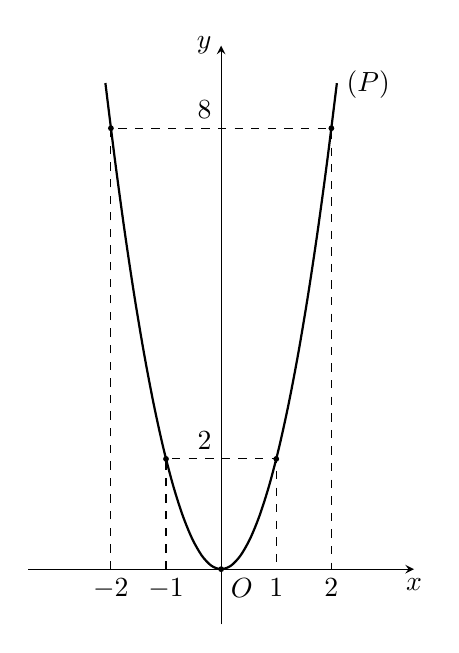
\begin{tikzpicture}[>=stealth, scale=0.7]
\draw[->] (-3.5,0) -- (3.5,0) node[below] {$x$};
\draw[->] (0,-1) -- (0,9.5) node[left] {$y$};
\fill (0,0) circle (1.5pt) node[below right] {$O$};
\draw[domain=-2.1:2.1, smooth, thick] plot (\x, {2*\x*\x});
\draw[dashed] (-2,0) node[below]{$-2$} |- (0,8) node[above left]{$8$} -| (2,0) node[below]{$2$};
\draw[dashed] (-1,0) node[below]{$-1$} |- (0,2) node[above left]{$2$} -| (1,0) node[below]{$1$};
\fill (-2,8) circle (1.5pt); \fill (2,8) circle (1.5pt);
\fill (-1,2) circle (1.5pt); \fill (1,2) circle (1.5pt);
\node[right] at (2.1, 8.8) {$(P)$};
\end{tikzpicture}
\end{center}
\textbf{b)} Tìm tọa độ các điểm $E$ \hfill \textit{(0,5 điểm)} \par
Gọi tọa độ điểm $E$ là $(x_E; y_E)$. Vì $E \in (P)$ nên $y_E = 2x_E^2$. \par
Theo đề bài, tổng hoành độ và tung độ bằng $3$, ta có phương trình:
$$ x_E + y_E = 3 $$
$$ \Leftrightarrow x_E + 2x_E^2 = 3 $$
$$ \Leftrightarrow 2x_E^2 + x_E - 3 = 0 $$
Vì $a + b + c = 2 + 1 + (-3) = 0$ nên phương trình có hai nghiệm:
$$ x_{E1} = 1; \quad x_{E2} = -\frac{3}{2} $$
Với $x_E = 1 \Rightarrow y_E = 2(1)^2 = 2$, ta được điểm $E_1(1; 2)$. \par
Với $x_E = -\frac{3}{2} \Rightarrow y_E = 2\left(-\frac{3}{2}\right)^2 = \frac{9}{2}$, ta được điểm $E_2\left(-\frac{3}{2}; \frac{9}{2}\right)$. \par
Vậy tọa độ các điểm $E$ cần tìm là $(1; 2)$ và $\left(-\frac{3}{2}; \frac{9}{2}\right)$.
}
\end{bt}

\begin{bt}%[TS10 1.0 1.4]%[ma:02d569b7]
Cho parabol $(P): y = 2x^2$ và đường thẳng $(d): y = x + 3$.
\textbf{a)} Vẽ đồ thị $(P)$ trên hệ trục tọa độ. \par
\textbf{b)} Tìm tọa độ giao điểm của $(P)$ và $(d)$ bằng phép tính.
\loigiai{
\textbf{a)} Vẽ đồ thị $(P): y = 2x^2$ \hfill \textit{(1,0 điểm)} \par
Bảng giá trị:
\begin{center}
\begin{tabular}{|c|c|c|c|c|c|}
\hline
$x$ & $-2$ & $-1$ & $0$ & $1$ & $2$ \\
\hline
$y = 2x^2$ & $8$ & $2$ & $0$ & $2$ & $8$ \\
\hline
\end{tabular}
\end{center}
Đồ thị hàm số $(P)$ là một đường parabol đi qua gốc tọa độ $O$, nhận trục $Oy$ làm trục đối xứng và nằm phía trên trục hoành.
\begin{center}
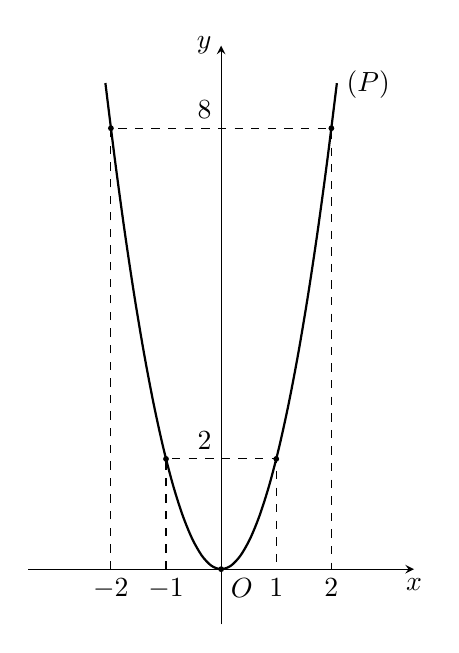
\begin{tikzpicture}[>=stealth, scale=0.7]
\draw[->] (-3.5,0) -- (3.5,0) node[below] {$x$};
\draw[->] (0,-1) -- (0,9.5) node[left] {$y$};
\fill (0,0) circle (1.5pt) node[below right] {$O$};
\draw[domain=-2.1:2.1, smooth, thick] plot (\x, {2*\x*\x});
\draw[dashed] (-2,0) node[below]{$-2$} |- (0,8) node[above left]{$8$} -| (2,0) node[below]{$2$};
\draw[dashed] (-1,0) node[below]{$-1$} |- (0,2) node[above left]{$2$} -| (1,0) node[below]{$1$};
\fill (-2,8) circle (1.5pt); \fill (2,8) circle (1.5pt);
\fill (-1,2) circle (1.5pt); \fill (1,2) circle (1.5pt);
\node[right] at (2.1, 8.8) {$(P)$};
\end{tikzpicture}
\end{center}
\textbf{b)} Tìm tọa độ giao điểm của $(P)$ và $(d)$ \hfill \textit{(0,5 điểm)} \par
Phương trình hoành độ giao điểm của $(P)$ và $(d)$ là:
$$ 2x^2 = x + 3 $$
$$ \Leftrightarrow 2x^2 - x - 3 = 0 $$
Vì $a - b + c = 2 - (-1) + (-3) = 0$ nên phương trình có hai nghiệm:
$$ x_1 = -1; \quad x_2 = \frac{3}{2} $$
Với $x = -1 \Rightarrow y = 2(-1)^2 = 2$. Ta được giao điểm thứ nhất là $(-1; 2)$. \par
Với $x = \frac{3}{2} \Rightarrow y = 2\left(\frac{3}{2}\right)^2 = \frac{9}{2}$. Ta được giao điểm thứ hai là $\left(\frac{3}{2}; \frac{9}{2}\right)$. \par
Vậy tọa độ giao điểm của $(P)$ và $(d)$ là $(-1; 2)$ và $\left(\frac{3}{2}; \frac{9}{2}\right)$.
}
\end{bt}


\begin{bt}%[TS10 1.0 1.5]%[ma:d4ba117e]
Cho parabol $(P): y = \frac{1}{2}x^2$.
\textbf{a)} Vẽ đồ thị $(P)$ trên mặt phẳng tọa độ. \par
\textbf{b)} Bằng phép tính, hãy kiểm tra xem các điểm $A(4; 8)$ và $B(-2; 3)$ có thuộc đồ thị $(P)$ hay không?
\loigiai{
\textbf{a)} Vẽ đồ thị $(P)$ \hfill \textit{(1,0 điểm)}\par
Bảng giá trị:
\begin{center}
\begin{tabular}{|c|c|c|c|c|c|}
\hline
$x$ & $-4$ & $-2$ & $0$ & $2$ & $4$ \\
\hline
$y = \frac{1}{2}x^2$ & $8$ & $2$ & $0$ & $2$ & $8$ \\
\hline
\end{tabular}
\end{center}
Đồ thị hàm số $(P)$ là một đường parabol đi qua gốc tọa độ $O$, nhận trục $Oy$ làm trục đối xứng và nằm phía trên trục hoành.
\begin{center}
\begin{tikzpicture}[>=stealth, scale=0.7]
\draw[->] (-5,0) -- (5,0) node[below] {$x$};
\draw[->] (0,-1) -- (0,9) node[left] {$y$};
\fill (0,0) circle (1.5pt) node[below right] {$O$};
\draw[domain=-4.2:4.2, smooth, thick] plot (\x, {0.5*\x*\x});
\draw[dashed] (-4,0) node[below]{$-4$} |- (0,8) node[above left]{$8$} -| (4,0) node[below]{$4$};
\draw[dashed] (-2,0) node[below]{$-2$} |- (0,2) node[above left]{$2$} -| (2,0) node[below]{$2$};
\fill (-4,8) circle (1.5pt); \fill (4,8) circle (1.5pt);
\fill (-2,2) circle (1.5pt); \fill (2,2) circle (1.5pt);
\node[right] at (4.2, 8.8) {$(P)$};
\end{tikzpicture}
\end{center}
\textbf{b)} Kiểm tra các điểm $A, B$ \hfill \textit{(0,5 điểm)}\par
Xét điểm $A(4; 8)$: Thay $x = 4$ vào hàm số của $(P)$, ta được:
$$ y = \frac{1}{2} \cdot 4^2 = \frac{1}{2} \cdot 16 = 8 $$
Giá trị này bằng với tung độ của điểm $A$, nên điểm $A(4; 8)$ thuộc $(P)$.\par
Xét điểm $B(-2; 3)$: Thay $x = -2$ vào hàm số của $(P)$, ta được:
$$ y = \frac{1}{2} \cdot (-2)^2 = \frac{1}{2} \cdot 4 = 2 $$
Giá trị này khác tung độ của điểm $B$ ($2 \neq 3$), nên điểm $B(-2; 3)$ không thuộc $(P)$.
}
\end{bt}

\begin{bt}%[TS10 1.0 1.6]%[ma:351f32e2]
Cho hàm số $y = x^2$ có đồ thị là parabol $(P)$.
\textbf{a)} Vẽ đồ thị $(P)$ trên hệ trục tọa độ. \par
\textbf{b)} Tìm tọa độ hai điểm $A, B$ thuộc $(P)$ (khác gốc tọa độ $O$) sao cho $A, B$ đối xứng nhau qua trục $Oy$ và tam giác $OAB$ vuông cân tại $O$.
\loigiai{
\textbf{a)} Vẽ đồ thị $(P)$ \hfill \textit{(1,0 điểm)}\par
Bảng giá trị:
\begin{center}
\begin{tabular}{|c|c|c|c|c|c|}
\hline
$x$ & $-2$ & $-1$ & $0$ & $1$ & $2$ \\
\hline
$y = x^2$ & $4$ & $1$ & $0$ & $1$ & $4$ \\
\hline
\end{tabular}
\end{center}
Đồ thị hàm số $(P)$ là đường parabol đi qua gốc tọa độ $O$, nhận trục $Oy$ làm trục đối xứng và nằm phía trên trục hoành.
\begin{center}
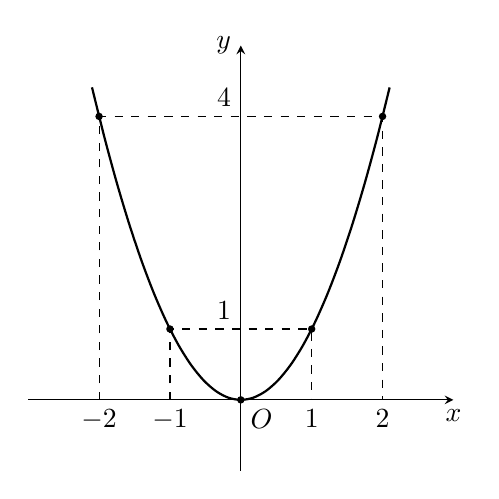
\begin{tikzpicture}[>=stealth, scale=0.9]
\draw[->] (-3,0) -- (3,0) node[below] {$x$};
\draw[->] (0,-1) -- (0,5) node[left] {$y$};
\fill (0,0) circle (1.5pt) node[below right] {$O$};
\draw[domain=-2.1:2.1, smooth, thick] plot (\x, {\x*\x});
\draw[dashed] (-2,0) node[below]{$-2$} |- (0,4) node[above left]{$4$} -| (2,0) node[below]{$2$};
\draw[dashed] (-1,0) node[below]{$-1$} |- (0,1) node[above left]{$1$} -| (1,0) node[below]{$1$};
\fill (-2,4) circle (1.5pt); \fill (2,4) circle (1.5pt);
\fill (-1,1) circle (1.5pt); \fill (1,1) circle (1.5pt);
\end{tikzpicture}
\end{center}
\textbf{b)} Tìm tọa độ hai điểm $A, B$ \hfill \textit{(0,5 điểm)}\par
Vì $A, B$ thuộc $(P)$ và đối xứng nhau qua trục $Oy$ nên ta gọi tọa độ điểm $B$ là $(x_0; x_0^2)$ với $x_0 > 0$. Khi đó tọa độ điểm $A$ là $(-x_0; x_0^2)$.\par
Độ dài đoạn thẳng $AB = x_0 - (-x_0) = 2x_0$.\par
Gọi $H$ là giao điểm của $AB$ và trục $Oy$, ta có $H(0; x_0^2)$. Suy ra $OH = x_0^2$.\par
Vì tam giác $OAB$ cân tại $O$ (do tính đối xứng) và vuông tại $O$, nên đường cao $OH$ đồng thời là đường trung tuyến ứng với cạnh huyền $AB$.
Do đó: $OH = \frac{1}{2}AB \Leftrightarrow x_0^2 = \frac{1}{2}(2x_0) \Leftrightarrow x_0^2 = x_0$.\par
Vì $x_0 > 0$ nên chia hai vế cho $x_0$, ta được $x_0 = 1$.\par
Với $x_0 = 1$, ta có $y_0 = 1^2 = 1$.\par
Vậy tọa độ hai điểm cần tìm là $A(-1; 1)$ và $B(1; 1)$.
}
\end{bt}

\begin{bt}%[TS10 1.0 1.5]%[ma:74517e8e]
Cho parabol $(P): y = -\frac{1}{4}x^2$.
\textbf{a)} Vẽ đồ thị $(P)$ trên mặt phẳng tọa độ $Oxy$. \par
\textbf{b)} Một vòm cầu có hình dạng parabol. Khi gắn hệ trục tọa độ sao cho đỉnh vòm cầu trùng với gốc tọa độ $O$ và vòm cầu nằm phía dưới trục hoành, người ta đo được bề rộng mặt cầu ở chân vòm là $8\text{ m}$ và chiều cao từ đỉnh vòm xuống chân vòm là $4\text{ m}$. Hỏi hình dạng của vòm cầu có khớp với đồ thị $(P)$ hay không? Vì sao?
\loigiai{
\textbf{a)} Vẽ đồ thị $(P)$ \hfill \textit{(1,0 điểm)}\par
Bảng giá trị:
\begin{center}
\begin{tabular}{|c|c|c|c|c|c|}
\hline
$x$ & $-4$ & $-2$ & $0$ & $2$ & $4$ \\
\hline
$y = -\frac{1}{4}x^2$ & $-4$ & $-1$ & $0$ & $-1$ & $-4$ \\
\hline
\end{tabular}
\end{center}
Đồ thị hàm số $(P)$ là đường parabol đi qua gốc tọa độ $O$, nhận trục $Oy$ làm trục đối xứng và nằm phía dưới trục hoành.
\begin{center}
\begin{tikzpicture}[>=stealth, scale=0.8]
\draw[->] (-5,0) -- (5,0) node[above] {$x$};
\draw[->] (0,-5) -- (0,1) node[right] {$y$};
\fill (0,0) circle (1.5pt) node[above right] {$O$};
\draw[domain=-4.2:4.2, smooth, thick] plot (\x, {-0.25*\x*\x});
\draw[dashed] (-4,0) node[above]{$-4$} |- (0,-4) node[below left]{$-4$} -| (4,0) node[above]{$4$};
\draw[dashed] (-2,0) node[above]{$-2$} |- (0,-1) node[below left]{$-1$} -| (2,0) node[above]{$2$};
\fill (-4,-4) circle (1.5pt); \fill (4,-4) circle (1.5pt);
\fill (-2,-1) circle (1.5pt); \fill (2,-1) circle (1.5pt);
\end{tikzpicture}
\end{center}
\textbf{b)} Kiểm tra sự khớp nhau của vòm cầu \hfill \textit{(0,5 điểm)}\par
Theo đề bài, bề rộng ở chân vòm là $8\text{ m}$, do tính đối xứng, mỗi bên gốc tọa độ rộng $4\text{ m}$, suy ra hoành độ chân vòm là $x = 4$ và $x = -4$.\par
Chiều cao từ đỉnh vòm (gốc $O$) xuống chân vòm là $4\text{ m}$ và vòm cầu nằm dưới trục hoành, nên tung độ của chân vòm là $y = -4$.\par
Như vậy, hai điểm ở chân vòm có tọa độ là $(4; -4)$ và $(-4; -4)$.\par
Ta kiểm tra xem điểm $(4; -4)$ có thuộc đồ thị $(P): y = -\frac{1}{4}x^2$ hay không:
Thay $x = 4$ vào phương trình $(P)$, ta có: $y = -\frac{1}{4} \cdot 4^2 = -\frac{1}{4} \cdot 16 = -4$ (đúng bằng tung độ của điểm).\par
Do parabol có tính đối xứng nên điểm $(-4; -4)$ cũng thuộc $(P)$.\par
Vậy hình dạng vòm cầu hoàn toàn khớp với đồ thị của $(P)$.
}
\end{bt}

\begin{bt}%[TS10 1.0 1.5]%[ma:2ccdfb7a]
Cho hàm số $y = -x^2$ có đồ thị là $(P)$.
\textbf{a)} Vẽ đồ thị $(P)$ trên hệ trục tọa độ. \par
\textbf{b)} Quỹ đạo của một tia nước từ một đài phun nước được mô phỏng bởi parabol $(P)$ (đơn vị trên các trục tính bằng mét). Một tia laser màu đỏ được chiếu ngang qua đài phun nước tại độ cao $y = -9$ (tức là cách đỉnh tia nước $9\text{ m}$ về phía dưới). Tính khoảng cách theo phương ngang giữa hai điểm mà tia nước cắt tia laser.
\loigiai{
\textbf{a)} Vẽ đồ thị $(P)$ \hfill \textit{(1,0 điểm)}\par
Bảng giá trị:
\begin{center}
\begin{tabular}{|c|c|c|c|c|c|}
\hline
$x$ & $-2$ & $-1$ & $0$ & $1$ & $2$ \\
\hline
$y = -x^2$ & $-4$ & $-1$ & $0$ & $-1$ & $-4$ \\
\hline
\end{tabular}
\end{center}
Đồ thị hàm số $(P)$ là đường parabol đi qua gốc tọa độ $O$, nhận trục $Oy$ làm trục đối xứng và nằm phía dưới trục hoành.
\begin{center}
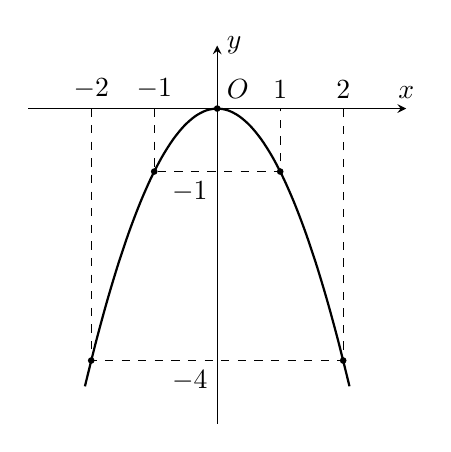
\begin{tikzpicture}[>=stealth, scale=0.8]
\draw[->] (-3,0) -- (3,0) node[above] {$x$};
\draw[->] (0,-5) -- (0,1) node[right] {$y$};
\fill (0,0) circle (1.5pt) node[above right] {$O$};
\draw[domain=-2.1:2.1, smooth, thick] plot (\x, {-\x*\x});
\draw[dashed] (-2,0) node[above]{$-2$} |- (0,-4) node[below left]{$-4$} -| (2,0) node[above]{$2$};
\draw[dashed] (-1,0) node[above]{$-1$} |- (0,-1) node[below left]{$-1$} -| (1,0) node[above]{$1$};
\fill (-2,-4) circle (1.5pt); \fill (2,-4) circle (1.5pt);
\fill (-1,-1) circle (1.5pt); \fill (1,-1) circle (1.5pt);
\end{tikzpicture}
\end{center}
\textbf{b)} Tính khoảng cách \hfill \textit{(0,5 điểm)}\par
Giao điểm của tia nước và tia laser là các điểm thuộc đồ thị $(P)$ có tung độ $y = -9$.\par
Thay $y = -9$ vào phương trình $(P)$, ta được:
$$ -x^2 = -9 \Leftrightarrow x^2 = 9 \Leftrightarrow x = 3 \text{ hoặc } x = -3 $$
Hai điểm cắt nhau có tọa độ lần lượt là $A(-3; -9)$ và $B(3; -9)$.\par
Khoảng cách theo phương ngang giữa hai điểm này là khoảng cách giữa hai hoành độ:
$$ AB = |3 - (-3)| = 6\text{ (m)} $$
Vậy khoảng cách theo phương ngang cần tìm là $6\text{ m}$.
}
\end{bt}

\begin{bt}%[TS10 1.0 1.6]%[ma:2d79bb6c]
Cho parabol $(P): y = \frac{1}{4}x^2$.
\textbf{a)} Vẽ đồ thị $(P)$ trên mặt phẳng tọa độ. \par
\textbf{b)} Gọi $A$ và $B$ là hai điểm thuộc $(P)$ có hoành độ lần lượt là $-2$ và $4$. Tính diện tích tam giác $OAB$.
\loigiai{
\textbf{a)} Vẽ đồ thị $(P)$ \hfill \textit{(1,0 điểm)}\par
Bảng giá trị:
\begin{center}
\begin{tabular}{|c|c|c|c|c|c|}
\hline
$x$ & $-4$ & $-2$ & $0$ & $2$ & $4$ \\
\hline
$y = \frac{1}{4}x^2$ & $4$ & $1$ & $0$ & $1$ & $4$ \\
\hline
\end{tabular}
\end{center}
Đồ thị hàm số $(P)$ là đường parabol đi qua gốc tọa độ $O$, nhận trục $Oy$ làm trục đối xứng và nằm phía trên trục hoành.
\begin{center}
\begin{tikzpicture}[>=stealth, scale=0.8]
\draw[->] (-5,0) -- (5,0) node[below] {$x$};
\draw[->] (0,-1) -- (0,5) node[left] {$y$};
\fill (0,0) circle (1.5pt) node[below right] {$O$};
\draw[domain=-4.2:4.2, smooth, thick] plot (\x, {0.25*\x*\x});
\draw[dashed] (-4,0) node[below]{$-4$} |- (0,4) node[above left]{$4$} -| (4,0) node[below]{$4$};
\draw[dashed] (-2,0) node[below]{$-2$} |- (0,1) node[above left]{$1$} -| (2,0) node[below]{$2$};
\fill (-4,4) circle (1.5pt); \fill (4,4) circle (1.5pt);
\fill (-2,1) circle (1.5pt); \fill (2,1) circle (1.5pt);
\end{tikzpicture}
\end{center}
\textbf{b)} Tính diện tích tam giác $OAB$ \hfill \textit{(0,5 điểm)}\par
Với $x_A = -2 \Rightarrow y_A = \frac{1}{4}(-2)^2 = 1$. Ta có $A(-2; 1)$.\par
Với $x_B = 4 \Rightarrow y_B = \frac{1}{4}(4)^2 = 4$. Ta có $B(4; 4)$.\par
Gọi phương trình đường thẳng $AB$ là $y = ax + b$.
Thay tọa độ $A, B$ vào, ta có hệ:
$$ \heva{&-2a + b = 1 \\ &4a + b = 4} \Leftrightarrow \heva{&6a = 3 \\ &b = 1 + 2a} \Leftrightarrow \heva{&a = \frac{1}{2} \\ &b = 2} $$
Đường thẳng $AB$ có phương trình $y = \frac{1}{2}x + 2$. Gọi $C$ là giao điểm của $AB$ với trục $Oy$, ta có $C(0; 2) \Rightarrow OC = 2$.\par
Diện tích tam giác $OAB$ được chia thành hai tam giác vuông $OAC$ và $OBC$ chung cạnh đáy $OC$:
$$ S_{OAB} = S_{OAC} + S_{OBC} = \frac{1}{2} \cdot OC \cdot |x_A| + \frac{1}{2} \cdot OC \cdot |x_B| $$
$$ S_{OAB} = \frac{1}{2} \cdot 2 \cdot |-2| + \frac{1}{2} \cdot 2 \cdot |4| = 2 + 4 = 6 \text{ (đvdt).} $$
}
\end{bt}

\begin{bt}%[TS10 1.0 1.5]%[ma:c6a45f7f]
Cho hàm số $y = 2x^2$ có đồ thị là $(P)$.
\textbf{a)} Vẽ $(P)$ trên hệ trục tọa độ. \par
\textbf{b)} Bằng phép tính, hãy xác định xem các điểm $E(3; 18)$ và $F(-\sqrt{2}; 4)$ có nằm trên đồ thị $(P)$ hay không?
\loigiai{
\textbf{a)} Vẽ đồ thị $(P)$ \hfill \textit{(1,0 điểm)}\par
Bảng giá trị:
\begin{center}
\begin{tabular}{|c|c|c|c|c|c|}
\hline
$x$ & $-2$ & $-1$ & $0$ & $1$ & $2$ \\
\hline
$y = 2x^2$ & $8$ & $2$ & $0$ & $2$ & $8$ \\
\hline
\end{tabular}
\end{center}
Đồ thị hàm số $(P)$ là đường parabol đi qua gốc tọa độ $O$, nhận trục $Oy$ làm trục đối xứng và nằm phía trên trục hoành.
\begin{center}
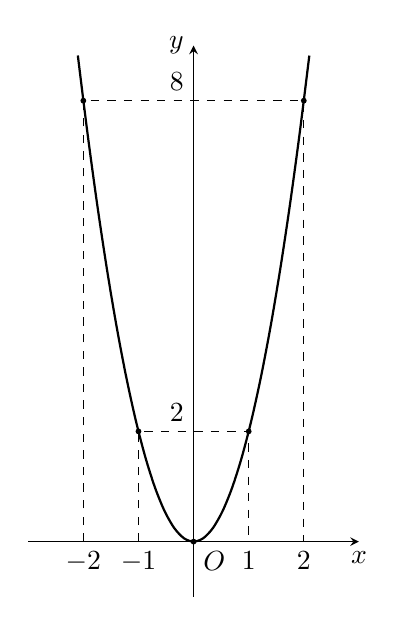
\begin{tikzpicture}[>=stealth, scale=0.7]
\draw[->] (-3,0) -- (3,0) node[below] {$x$};
\draw[->] (0,-1) -- (0,9) node[left] {$y$};
\fill (0,0) circle (1.5pt) node[below right] {$O$};
\draw[domain=-2.1:2.1, smooth, thick] plot (\x, {2*\x*\x});
\draw[dashed] (-2,0) node[below]{$-2$} |- (0,8) node[above left]{$8$} -| (2,0) node[below]{$2$};
\draw[dashed] (-1,0) node[below]{$-1$} |- (0,2) node[above left]{$2$} -| (1,0) node[below]{$1$};
\fill (-2,8) circle (1.5pt); \fill (2,8) circle (1.5pt);
\fill (-1,2) circle (1.5pt); \fill (1,2) circle (1.5pt);
\end{tikzpicture}
\end{center}
\textbf{b)} Xác định các điểm $E, F$ \hfill \textit{(0,5 điểm)}\par
Xét điểm $E(3; 18)$: Thay hoành độ $x = 3$ vào hàm số của $(P)$, ta được:
$$ y = 2 \cdot 3^2 = 2 \cdot 9 = 18 $$
Đúng bằng tung độ của điểm $E$, nên điểm $E(3; 18)$ nằm trên $(P)$.\par
Xét điểm $F(-\sqrt{2}; 4)$: Thay hoành độ $x = -\sqrt{2}$ vào hàm số của $(P)$, ta được:
$$ y = 2 \cdot (-\sqrt{2})^2 = 2 \cdot 2 = 4 $$
Đúng bằng tung độ của điểm $F$, nên điểm $F(-\sqrt{2}; 4)$ cũng nằm trên $(P)$.\par
Vậy cả hai điểm $E$ và $F$ đều nằm trên đồ thị $(P)$.
}
\end{bt}

\begin{bt}%[TS10 1.0 1.5]%[ma:05be1f49]
Cho parabol $(P): y = -\frac{1}{2}x^2$.
\textbf{a)} Vẽ đồ thị $(P)$ trên hệ trục tọa độ. \par
\textbf{b)} Một cổng vòm có dạng parabol $(P)$ với đơn vị đo trên các trục là mét. Biết rằng mặt đường đi ngang qua vòm cầu ứng với đường thẳng $y = -2$. Tính bề rộng của mặt đường đi dưới cổng vòm đó.
\loigiai{
\textbf{a)} Vẽ đồ thị $(P)$ \hfill \textit{(1,0 điểm)}\par
Bảng giá trị:
\begin{center}
\begin{tabular}{|c|c|c|c|c|c|}
\hline
$x$ & $-4$ & $-2$ & $0$ & $2$ & $4$ \\
\hline
$y = -\frac{1}{2}x^2$ & $-8$ & $-2$ & $0$ & $-2$ & $-8$ \\
\hline
\end{tabular}
\end{center}
Đồ thị hàm số $(P)$ là đường parabol đi qua gốc tọa độ $O$, nhận trục $Oy$ làm trục đối xứng và nằm phía dưới trục hoành.
\begin{center}
\begin{tikzpicture}[>=stealth, scale=0.7]
\draw[->] (-5,0) -- (5,0) node[above] {$x$};
\draw[->] (0,-9) -- (0,1) node[right] {$y$};
\fill (0,0) circle (1.5pt) node[above right] {$O$};
\draw[domain=-4.2:4.2, smooth, thick] plot (\x, {-0.5*\x*\x});
\draw[dashed] (-4,0) node[above]{$-4$} |- (0,-8) node[below left]{$-8$} -| (4,0) node[above]{$4$};
\draw[dashed] (-2,0) node[above]{$-2$} |- (0,-2) node[below left]{$-2$} -| (2,0) node[above]{$2$};
\fill (-4,-8) circle (1.5pt); \fill (4,-8) circle (1.5pt);
\fill (-2,-2) circle (1.5pt); \fill (2,-2) circle (1.5pt);
\end{tikzpicture}
\end{center}
\textbf{b)} Tính bề rộng mặt đường \hfill \textit{(0,5 điểm)}\par
Mặt đường tương ứng với các điểm trên $(P)$ có tung độ $y = -2$. Ta xét phương trình:
$$ -\frac{1}{2}x^2 = -2 \Leftrightarrow x^2 = 4 \Leftrightarrow \heva{&x = 2 \\ &x = -2} $$
Do đó, cổng vòm chạm mặt đường tại hai điểm có tọa độ $(2; -2)$ và $(-2; -2)$.\par
Bề rộng của mặt đường đi dưới cổng vòm chính là khoảng cách giữa hai hoành độ này:
$$ \text{Bề rộng} = 2 - (-2) = 4 \text{ (m)} $$
Vậy bề rộng của mặt đường đi dưới cổng vòm là $4\text{ m}$.
}
\end{bt}

\begin{bt}%[TS10 1.0 1.6]%[ma:0e41f170]
Cho hàm số $y = -2x^2$ có đồ thị là $(P)$.
\textbf{a)} Vẽ $(P)$ trên mặt phẳng tọa độ $Oxy$. \par
\textbf{b)} Đường thẳng $d: y = -8$ cắt đồ thị $(P)$ tại hai điểm phân biệt $M, N$. Tính chu vi tam giác $OMN$.
\loigiai{
\textbf{a)} Vẽ đồ thị $(P)$ \hfill \textit{(1,0 điểm)}\par
Bảng giá trị:
\begin{center}
\begin{tabular}{|c|c|c|c|c|c|}
\hline
$x$ & $-2$ & $-1$ & $0$ & $1$ & $2$ \\
\hline
$y = -2x^2$ & $-8$ & $-2$ & $0$ & $-2$ & $-8$ \\
\hline
\end{tabular}
\end{center}
Đồ thị hàm số $(P)$ là đường parabol đi qua gốc tọa độ $O$, nhận trục $Oy$ làm trục đối xứng và nằm phía dưới trục hoành.
\begin{center}
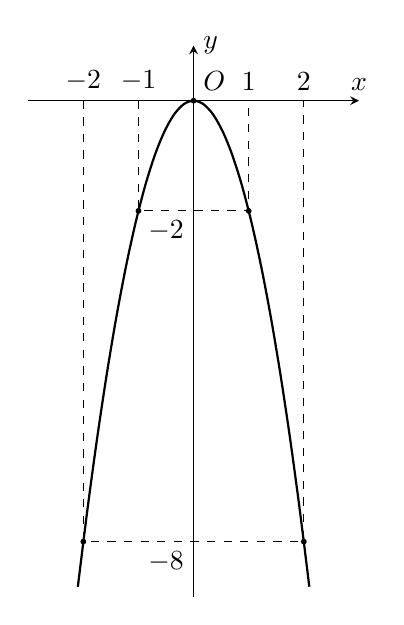
\begin{tikzpicture}[>=stealth, scale=0.7]
\draw[->] (-3,0) -- (3,0) node[above] {$x$};
\draw[->] (0,-9) -- (0,1) node[right] {$y$};
\fill (0,0) circle (1.5pt) node[above right] {$O$};
\draw[domain=-2.1:2.1, smooth, thick] plot (\x, {-2*\x*\x});
\draw[dashed] (-2,0) node[above]{$-2$} |- (0,-8) node[below left]{$-8$} -| (2,0) node[above]{$2$};
\draw[dashed] (-1,0) node[above]{$-1$} |- (0,-2) node[below left]{$-2$} -| (1,0) node[above]{$1$};
\fill (-2,-8) circle (1.5pt); \fill (2,-8) circle (1.5pt);
\fill (-1,-2) circle (1.5pt); \fill (1,-2) circle (1.5pt);
\end{tikzpicture}
\end{center}
\textbf{b)} Tính chu vi tam giác $OMN$ \hfill \textit{(0,5 điểm)}\par
Phương trình hoành độ giao điểm của $(P)$ và $d$:
$$ -2x^2 = -8 \Leftrightarrow x^2 = 4 \Leftrightarrow x = \pm 2 $$
Ta được tọa độ hai giao điểm là $M(-2; -8)$ và $N(2; -8)$.\par
Độ dài cạnh $MN = 2 - (-2) = 4$.\par
Áp dụng định lý Pythagore để tính $OM$ và $ON$ (với $OM = ON$ do tính đối xứng):
$$ OM = \sqrt{(-2)^2 + (-8)^2} = \sqrt{4 + 64} = \sqrt{68} = 2\sqrt{17} $$
Do đó $ON = 2\sqrt{17}$.\par
Chu vi tam giác $OMN$ là:
$$ P = OM + ON + MN = 2\sqrt{17} + 2\sqrt{17} + 4 = 4 + 4\sqrt{17} \text{ (đvđd).} $$
}
\end{bt}

\begin{bt}%[TS10 1.0 1.5]%[ma:6cfca531]
Cho parabol $(P): y = \frac{x^2}{2}$.
\textbf{a)} Vẽ đồ thị $(P)$ trên hệ trục tọa độ. \par
\textbf{b)} Tìm tham số $m$ để điểm $K(2m; 8)$ thuộc đồ thị $(P)$.
\loigiai{
\textbf{a)} Vẽ đồ thị $(P)$ \hfill \textit{(1,0 điểm)}\par
Bảng giá trị:
\begin{center}
\begin{tabular}{|c|c|c|c|c|c|}
\hline
$x$ & $-4$ & $-2$ & $0$ & $2$ & $4$ \\
\hline
$y = \frac{x^2}{2}$ & $8$ & $2$ & $0$ & $2$ & $8$ \\
\hline
\end{tabular}
\end{center}
Đồ thị hàm số $(P)$ là đường parabol đi qua gốc tọa độ $O$, nhận trục $Oy$ làm trục đối xứng và nằm phía trên trục hoành.
\begin{center}
\begin{tikzpicture}[>=stealth, scale=0.7]
\draw[->] (-5,0) -- (5,0) node[below] {$x$};
\draw[->] (0,-1) -- (0,9) node[left] {$y$};
\fill (0,0) circle (1.5pt) node[below right] {$O$};
\draw[domain=-4.2:4.2, smooth, thick] plot (\x, {0.5*\x*\x});
\draw[dashed] (-4,0) node[below]{$-4$} |- (0,8) node[above left]{$8$} -| (4,0) node[below]{$4$};
\draw[dashed] (-2,0) node[below]{$-2$} |- (0,2) node[above left]{$2$} -| (2,0) node[below]{$2$};
\fill (-4,8) circle (1.5pt); \fill (4,8) circle (1.5pt);
\fill (-2,2) circle (1.5pt); \fill (2,2) circle (1.5pt);
\end{tikzpicture}
\end{center}
\textbf{b)} Tìm tham số $m$ \hfill \textit{(0,5 điểm)}\par
Vì điểm $K(2m; 8)$ thuộc đồ thị $(P): y = \frac{x^2}{2}$, ta thay $x = 2m$ và $y = 8$ vào hàm số, ta được:
$$ 8 = \frac{(2m)^2}{2} $$
$$ \Leftrightarrow 8 = \frac{4m^2}{2} $$
$$ \Leftrightarrow 8 = 2m^2 $$
$$ \Leftrightarrow m^2 = 4 $$
$$ \Leftrightarrow m = 2 \text{ hoặc } m = -2 $$
Vậy các giá trị của tham số $m$ cần tìm là $m = 2$ hoặc $m = -2$.
}
\end{bt}

\begin{bt}%[TS10 1.0 1.5]%[ma:cd8cc7a4]
Cho hàm số $y = x^2$ có đồ thị $(P)$.
\textbf{a)} Vẽ đồ thị $(P)$ trên hệ trục tọa độ. \par
\textbf{b)} Mặt cắt mặt trước của một chảo ăng-ten vệ tinh có hình dạng parabol $(P)$ (đơn vị trên các trục tọa độ tính bằng đê-xi-mét). Người ta đo được chiều sâu của chảo (tính từ mặt đáy ở đỉnh $O$ lên đến miệng chảo) là $4\text{ dm}$. Hỏi đường kính miệng chảo ăng-ten đó bằng bao nhiêu?
\loigiai{
\textbf{a)} Vẽ đồ thị $(P)$ \hfill \textit{(1,0 điểm)}\par
Bảng giá trị:
\begin{center}
\begin{tabular}{|c|c|c|c|c|c|}
\hline
$x$ & $-2$ & $-1$ & $0$ & $1$ & $2$ \\
\hline
$y = x^2$ & $4$ & $1$ & $0$ & $1$ & $4$ \\
\hline
\end{tabular}
\end{center}
Đồ thị hàm số $(P)$ là đường parabol đi qua gốc tọa độ $O$, nhận trục $Oy$ làm trục đối xứng và nằm phía trên trục hoành.
\begin{center}
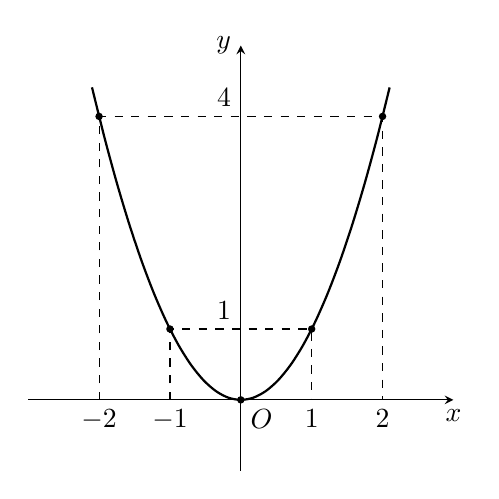
\begin{tikzpicture}[>=stealth, scale=0.9]
\draw[->] (-3,0) -- (3,0) node[below] {$x$};
\draw[->] (0,-1) -- (0,5) node[left] {$y$};
\fill (0,0) circle (1.5pt) node[below right] {$O$};
\draw[domain=-2.1:2.1, smooth, thick] plot (\x, {\x*\x});
\draw[dashed] (-2,0) node[below]{$-2$} |- (0,4) node[above left]{$4$} -| (2,0) node[below]{$2$};
\draw[dashed] (-1,0) node[below]{$-1$} |- (0,1) node[above left]{$1$} -| (1,0) node[below]{$1$};
\fill (-2,4) circle (1.5pt); \fill (2,4) circle (1.5pt);
\fill (-1,1) circle (1.5pt); \fill (1,1) circle (1.5pt);
\end{tikzpicture}
\end{center}
\textbf{b)} Tính đường kính miệng chảo \hfill \textit{(0,5 điểm)}\par
Chiều sâu của chảo là khoảng cách từ đỉnh đến miệng chảo, tức là tương ứng với tung độ $y = 4$.\par
Miệng chảo ứng với các điểm trên $(P)$ có tung độ $y = 4$. Thay vào phương trình hàm số, ta có:
$$ x^2 = 4 \Leftrightarrow x = 2 \text{ hoặc } x = -2 $$
Hai điểm ở mép miệng chảo có tọa độ là $(2; 4)$ và $(-2; 4)$.\par
Đường kính miệng chảo chính là khoảng cách giữa hai hoành độ này:
$$ d = 2 - (-2) = 4 \text{ (dm)} $$
Vậy đường kính miệng chảo ăng-ten đó là $4\text{ dm}$.
}
\end{bt}


\begin{bt}%[TS10 1.0 1.1]%[ma:cca11f94]
% nguon: Đề thi chính thức Tuyển sinh 10 TP.HCM năm học 2025-2026 – Bài 1
Cho hàm số $y = \dfrac{x^2}{2}$ có đồ thị $(P)$.
\begin{enumerate}[a)]
	\item Vẽ đồ thị $(P)$ trên hệ trục toạ độ.
	\item Tìm toạ độ các điểm thuộc $(P)$ có tung độ bằng $18$.
\end{enumerate}
\loigiai{
\begin{enumerate}[a)]
	\item Bảng giá trị tương ứng giữa $x$ và $y$ của hàm số $y = \dfrac{x^2}{2}$:
	\begin{center}
	\begin{tabular}{|c|c|c|c|c|c|}
	\hline
	$x$ & $-4$ & $-2$ & $0$ & $2$ & $4$ \\
	\hline
	$y = \dfrac{x^2}{2}$ & $8$ & $2$ & $0$ & $2$ & $8$ \\
	\hline
	\end{tabular}
	\end{center}
	Đồ thị $(P)$ là một parabol đi qua gốc toạ độ $O(0; 0)$, nhận trục tung $Oy$ làm trục đối xứng và nằm phía trên trục hoành.
	\item Điểm thuộc $(P)$ có tung độ bằng $18$ thoả mãn phương trình:
	$18 = \dfrac{x^2}{2} \Leftrightarrow x^2 = 36 \Leftrightarrow x = 6$ hoặc $x = -6$.\\
	Vậy toạ độ các điểm thoả mãn yêu cầu đề bài là $(6; 18)$ và $(-6; 18)$.
\end{enumerate}
}
\end{bt}

\begin{bt}%[TS10 1.0 1.2]%[ma:390e4e76]
% nguon: Đề thi tham khảo Tuyển sinh 10 TP.HCM – Phụ lục Sở GD&ĐT TP.HCM – Bài 1
Cho hàm số $y = \dfrac{x^2}{2}$ có đồ thị $(P)$.
\begin{enumerate}[a)]
	\item Vẽ đồ thị $(P)$ của hàm số trên.
	\item Tìm những điểm $M$ thuộc $(P)$ có tung độ và hoành độ bằng nhau.
\end{enumerate}
\loigiai{
\begin{enumerate}[a)]
	\item Bảng giá trị tương ứng giữa $x$ và $y$ của hàm số $y = \dfrac{x^2}{2}$:
	\begin{center}
	\begin{tabular}{|c|c|c|c|c|c|}
	\hline
	$x$ & $-4$ & $-2$ & $0$ & $2$ & $4$ \\
	\hline
	$y = \dfrac{x^2}{2}$ & $8$ & $2$ & $0$ & $2$ & $8$ \\
	\hline
	\end{tabular}
	\end{center}
	Đồ thị $(P)$ là một đường parabol đi qua gốc toạ độ $O(0; 0)$, nhận trục tung $Oy$ làm trục đối xứng và nằm phía trên trục hoành.
	\item Điểm $M(x_M; y_M)$ thuộc $(P)$ có tung độ và hoành độ bằng nhau thoả mãn:
	$y_M = x_M \Leftrightarrow \dfrac{x_M^2}{2} = x_M \Leftrightarrow x_M^2 - 2x_M = 0 \Leftrightarrow x_M(x_M - 2) = 0 \Leftrightarrow \left[\begin{aligned} x_M &= 0 \Rightarrow y_M = 0 \\ x_M &= 2 \Rightarrow y_M = 2. \end{aligned}\right.$\\
	Vậy có hai điểm thoả mãn yêu cầu đề bài là $M_1(0; 0)$ và $M_2(2; 2)$.
\end{enumerate}
}
\end{bt}

\begin{bt}%[TS10 1.0 1.2]%[ma:3f93dc01]
% nguon: Đề tham khảo Tuyển sinh 10 TP.HCM 2025-2026 – Quận 1 – Đề 1 – Bài 1
Cho parabol $(P): y = \dfrac{x^2}{2}$.
\begin{enumerate}[a)]
	\item Vẽ đồ thị $(P)$ của hàm số trên.
	\item Tìm trên $(P)$ những điểm $M$ sao cho tung độ gấp đôi hoành độ.
\end{enumerate}
\loigiai{
\begin{enumerate}[a)]
	\item Bảng giá trị tương ứng giữa $x$ và $y$ của hàm số $y = \dfrac{x^2}{2}$:
	\begin{center}
	\begin{tabular}{|c|c|c|c|c|c|}
	\hline
	$x$ & $-4$ & $-2$ & $0$ & $2$ & $4$ \\
	\hline
	$y = \dfrac{x^2}{2}$ & $8$ & $2$ & $0$ & $2$ & $8$ \\
	\hline
	\end{tabular}
	\end{center}
	Đồ thị $(P)$ là một đường parabol đi qua gốc toạ độ $O(0; 0)$, nhận trục tung $Oy$ làm trục đối xứng và nằm phía trên trục hoành.
	\item Điểm $M(x; y)$ thuộc $(P)$ có tung độ gấp đôi hoành độ thoả mãn:
	$y = 2x \Leftrightarrow \dfrac{x^2}{2} = 2x \Leftrightarrow x^2 - 4x = 0 \Leftrightarrow x(x - 4) = 0 \Leftrightarrow \left[\begin{aligned} x &= 0 \Rightarrow y = 0 \\ x &= 4 \Rightarrow y = 8. \end{aligned}\right.$\\
	Vậy có hai điểm thoả mãn yêu cầu đề bài là $M_1(0; 0)$ và $M_2(4; 8)$.
\end{enumerate}
}
\end{bt}

\begin{bt}%[TS10 1.0 1.2]%[ma:63feb2d0]
% nguon: Đề tham khảo Tuyển sinh 10 TP.HCM 2025-2026 – Quận 1 – Đề 2 – Bài 1
Cho parabol $(P): y = -\dfrac{1}{2}x^2$.
\begin{enumerate}[a)]
	\item Vẽ đồ thị $(P)$ trên mặt phẳng toạ độ $Oxy$.
	\item Tìm các điểm $M$ thuộc đồ thị $(P)$ sao cho $M$ có hoành độ và tung độ là hai số đối nhau.
\end{enumerate}
\loigiai{
\begin{enumerate}[a)]
	\item Bảng giá trị tương ứng giữa $x$ và $y$ của hàm số $y = -\dfrac{1}{2}x^2$:
	\begin{center}
	\begin{tabular}{|c|c|c|c|c|c|}
	\hline
	$x$ & $-4$ & $-2$ & $0$ & $2$ & $4$ \\
	\hline
	$y = -\dfrac{1}{2}x^2$ & $-8$ & $-2$ & $0$ & $-2$ & $-8$ \\
	\hline
	\end{tabular}
	\end{center}
	Đồ thị $(P)$ là một đường parabol có đỉnh là gốc toạ độ $O(0; 0)$, nhận trục tung $Oy$ làm trục đối xứng và nằm phía dưới trục hoành.
	\item Điểm $M(x; y)$ thuộc $(P)$ có hoành độ và tung độ là hai số đối nhau thoả mãn:
	$y = -x \Leftrightarrow -\dfrac{1}{2}x^2 = -x \Leftrightarrow x^2 - 2x = 0 \Leftrightarrow x(x - 2) = 0 \Leftrightarrow \left[\begin{aligned} x &= 0 \Rightarrow y = 0 \\ x &= 2 \Rightarrow y = -2. \end{aligned}\right.$\\
	Vậy có hai điểm thoả mãn là $M_1(0; 0)$ và $M_2(2; -2)$.
\end{enumerate}
}
\end{bt}

\begin{bt}%[TS10 1.0 1.2]%[ma:fc5c4aa0]
% nguon: Đề tham khảo Tuyển sinh 10 TP.HCM 2025-2026 – Quận 3 – Đề 1 – Bài 1
Cho parabol $(P): y = \dfrac{1}{2}x^2$.
\begin{enumerate}[a)]
	\item Vẽ đồ thị $(P)$ trên mặt phẳng toạ độ $Oxy$.
	\item Tìm điểm $K$ khác gốc toạ độ thuộc $(P)$ sao cho tung độ gấp đôi hoành độ.
\end{enumerate}
\loigiai{
\begin{enumerate}[a)]
	\item Bảng giá trị tương ứng giữa $x$ và $y$ của hàm số $y = \dfrac{1}{2}x^2$:
	\begin{center}
	\begin{tabular}{|c|c|c|c|c|c|}
	\hline
	$x$ & $-4$ & $-2$ & $0$ & $2$ & $4$ \\
	\hline
	$y = \dfrac{1}{2}x^2$ & $8$ & $2$ & $0$ & $2$ & $8$ \\
	\hline
	\end{tabular}
	\end{center}
	Đồ thị $(P)$ là một parabol đi qua gốc toạ độ $O(0; 0)$, nhận trục tung $Oy$ làm trục đối xứng và nằm phía trên trục hoành.
	\item Điểm $K(x; y)$ thuộc $(P)$ có tung độ gấp đôi hoành độ thoả mãn:
	$y = 2x \Leftrightarrow \dfrac{1}{2}x^2 = 2x \Leftrightarrow x^2 - 4x = 0 \Leftrightarrow x(x - 4) = 0 \Leftrightarrow \left[\begin{aligned} x &= 0 \Rightarrow y = 0 \\ x &= 4 \Rightarrow y = 8. \end{aligned}\right.$\\
	Vì điểm $K$ khác gốc toạ độ nên $x \neq 0$. Do đó $K(4; 8)$.
\end{enumerate}
}
\end{bt}

\begin{bt}%[TS10 1.0 1.2]%[ma:24ffbcaa]
% nguon: Đề tham khảo Tuyển sinh 10 TP.HCM 2025-2026 – Quận 3 – Đề 2 – Bài 1
Cho parabol $(P): y = -\dfrac{x^2}{4}$.
\begin{enumerate}[a)]
	\item Vẽ đồ thị $(P)$ trên hệ trục toạ độ $Oxy$.
	\item Tìm toạ độ những điểm $M$ thuộc $(P)$ có tung độ gấp $3$ lần hoành độ.
\end{enumerate}
\loigiai{
\begin{enumerate}[a)]
	\item Bảng giá trị tương ứng giữa $x$ và $y$ của hàm số $y = -\dfrac{x^2}{4}$:
	\begin{center}
	\begin{tabular}{|c|c|c|c|c|c|}
	\hline
	$x$ & $-4$ & $-2$ & $0$ & $2$ & $4$ \\
	\hline
	$y = -\dfrac{x^2}{4}$ & $-4$ & $-1$ & $0$ & $-1$ & $-4$ \\
	\hline
	\end{tabular}
	\end{center}
	Đồ thị $(P)$ là một parabol có đỉnh tại gốc toạ độ $O(0; 0)$, nhận trục tung $Oy$ làm trục đối xứng và nằm phía dưới trục hoành.
	\item Điểm $M(x; y)$ thuộc $(P)$ có tung độ gấp $3$ lần hoành độ thoả mãn:
	$y = 3x \Leftrightarrow -\dfrac{x^2}{4} = 3x \Leftrightarrow x^2 + 12x = 0 \Leftrightarrow x(x + 12) = 0 \Leftrightarrow \left[\begin{aligned} x &= 0 \Rightarrow y = 0 \\ x &= -12 \Rightarrow y = -36. \end{aligned}\right.$\\
	Vậy có hai điểm thoả mãn yêu cầu đề bài là $M_1(0; 0)$ và $M_2(-12; -36)$.
\end{enumerate}
}
\end{bt}

\begin{bt}%[TS10 1.0 1.2]%[ma:d700d684]
% nguon: Đề tham khảo Tuyển sinh 10 TP.HCM 2025-2026 – Quận 4 – Đề 1 – Bài 1
Cho parabol $(P): y = -\dfrac{1}{2}x^2$.
\begin{enumerate}[a)]
	\item Vẽ đồ thị $(P)$ trên hệ trục toạ độ $Oxy$.
	\item Tìm toạ độ những điểm $A$ thuộc $(P)$ biết rằng tung độ của nó gấp đôi hoành độ.
\end{enumerate}
\loigiai{
\begin{enumerate}[a)]
	\item Bảng giá trị tương ứng giữa $x$ và $y$ của hàm số $y = -\dfrac{1}{2}x^2$:
	\begin{center}
	\begin{tabular}{|c|c|c|c|c|c|}
	\hline
	$x$ & $-4$ & $-2$ & $0$ & $2$ & $4$ \\
	\hline
	$y = -\dfrac{1}{2}x^2$ & $-8$ & $-2$ & $0$ & $-2$ & $-8$ \\
	\hline
	\end{tabular}
	\end{center}
	Đồ thị $(P)$ là một parabol có đỉnh tại gốc toạ độ $O(0; 0)$, nhận trục tung $Oy$ làm trục đối xứng và nằm phía dưới trục hoành.
	\item Điểm $A(x; y)$ thuộc $(P)$ có tung độ gấp đôi hoành độ thoả mãn:
	$y = 2x \Leftrightarrow -\dfrac{1}{2}x^2 = 2x \Leftrightarrow x^2 + 4x = 0 \Leftrightarrow x(x + 4) = 0 \Leftrightarrow \left[\begin{aligned} x &= 0 \Rightarrow y = 0 \\ x &= -4 \Rightarrow y = -8. \end{aligned}\right.$\\
	Vậy có hai điểm thoả mãn là $A_1(0; 0)$ và $A_2(-4; -8)$.
\end{enumerate}
}
\end{bt}

\begin{bt}%[TS10 1.0 1.2]%[ma:c2269a21]
% nguon: Đề tham khảo Tuyển sinh 10 TP.HCM 2025-2026 – Quận 4 – Đề 2 – Bài 1
Cho hàm số $y = \dfrac{1}{2}x^2$ có đồ thị là parabol $(P)$.
\begin{enumerate}[a)]
	\item Vẽ đồ thị $(P)$ trên mặt phẳng toạ độ $Oxy$.
	\item Tìm điểm $A$ thuộc $(P)$ sao cho hoành độ gấp hai lần tung độ.
\end{enumerate}
\loigiai{
\begin{enumerate}[a)]
	\item Bảng giá trị tương ứng giữa $x$ và $y$ của hàm số $y = \dfrac{1}{2}x^2$:
	\begin{center}
	\begin{tabular}{|c|c|c|c|c|c|}
	\hline
	$x$ & $-4$ & $-2$ & $0$ & $2$ & $4$ \\
	\hline
	$y = \dfrac{1}{2}x^2$ & $8$ & $2$ & $0$ & $2$ & $8$ \\
	\hline
	\end{tabular}
	\end{center}
	Đồ thị $(P)$ là một parabol có đỉnh tại gốc toạ độ $O(0; 0)$, nhận trục tung $Oy$ làm trục đối xứng và nằm phía trên trục hoành.
	\item Điểm $A(x; y)$ thuộc $(P)$ có hoành độ gấp hai lần tung độ thoả mãn:
	$x = 2y \Leftrightarrow x = 2\left(\dfrac{1}{2}x^2\right) \Leftrightarrow x = x^2 \Leftrightarrow x^2 - x = 0 \Leftrightarrow x(x - 1) = 0 \Leftrightarrow \left[\begin{aligned} x &= 0 \Rightarrow y = 0 \\ x &= 1 \Rightarrow y = \dfrac{1}{2}. \end{aligned}\right.$\\
	Vậy có hai điểm thoả mãn là $A_1(0; 0)$ và $A_2\left(1; \dfrac{1}{2}\right)$.
\end{enumerate}
}
\end{bt}

\begin{bt}%[TS10 1.0 1.2]%[ma:2da8ea50]
% nguon: Đề tham khảo Tuyển sinh 10 TP.HCM 2025-2026 – Quận 5 – Đề 1 – Bài 1
Cho parabol $(P)\colon y = -\dfrac{1}{2}x^2$.
\begin{enumerate}[a)]
    \item Vẽ $(P)$ trên hệ trục tọa độ $Oxy$.
    \item Tìm tọa độ các điểm $A$ thuộc $(P)$ có hoành độ gấp hai lần tung độ.
\end{enumerate}
\loigiai{
\begin{enumerate}[a)]
    \item Bảng giá trị tương ứng của $x$ và $y$:
    \begin{center}
    \begin{tabular}{|c|c|c|c|c|c|}
        \hline
        $x$ & $-4$ & $-2$ & $0$ & $2$ & $4$ \\ \hline
        $y = -\dfrac{1}{2}x^2$ & $-8$ & $-2$ & $0$ & $-2$ & $-8$ \\ \hline
    \end{tabular}
    \end{center}
    Đồ thị $(P)$ là một parabol đi qua gốc tọa độ $O(0;0)$, nhận trục $Oy$ làm trục đối xứng và nằm phía dưới trục hoành.
    \item Gọi điểm $A(x_A; y_A) \in (P)$ thỏa mãn hoành độ gấp hai lần tung độ, tức là $x_A = 2y_A \Leftrightarrow y_A = \dfrac{x_A}{2}$.\\
    Vì $A \in (P)$ nên ta có phương trình:
    $\dfrac{x_A}{2} = -\dfrac{1}{2}x_A^2 \Leftrightarrow x_A^2 + x_A = 0 \Leftrightarrow x_A(x_A + 1) = 0 \Leftrightarrow \left[\begin{aligned} &x_A = 0 \\ &x_A = -1. \end{aligned}\right.$\\
    Với $x_A = 0 \Rightarrow y_A = 0$, ta được điểm $A_1(0; 0)$.\\
    Với $x_A = -1 \Rightarrow y_A = -\dfrac{1}{2}$, ta được điểm $A_2\left(-1; -\dfrac{1}{2}\right)$.\\
    Vậy tọa độ các điểm cần tìm là $(0; 0)$ và $\left(-1; -\dfrac{1}{2}\right)$.
\end{enumerate}
}
\end{bt}

\begin{bt}%[TS10 1.0 1.1]%[ma:daf2d411]
% nguon: Đề tham khảo Tuyển sinh 10 TP.HCM 2025-2026 – Quận 5 – Đề 2 – Bài 1
Cho parabol $(P)\colon y = -\dfrac{1}{2}x^2$.
\begin{enumerate}[a)]
    \item Vẽ đồ thị $(P)$.
    \item Tìm các điểm $M$ thuộc $(P)$ sao cho tung độ bằng $-8$.
\end{enumerate}
\loigiai{
\begin{enumerate}[a)]
    \item Bảng giá trị tương ứng của $x$ và $y$:
    \begin{center}
    \begin{tabular}{|c|c|c|c|c|c|}
        \hline
        $x$ & $-4$ & $-2$ & $0$ & $2$ & $4$ \\ \hline
        $y = -\dfrac{1}{2}x^2$ & $-8$ & $-2$ & $0$ & $-2$ & $-8$ \\ \hline
    \end{tabular}
    \end{center}
    Đồ thị $(P)$ là một parabol đi qua gốc tọa độ $O(0;0)$, nhận trục $Oy$ làm trục đối xứng và bề lõm quay xuống dưới.
    \item Điểm $M(x_M; y_M) \in (P)$ có tung độ $y_M = -8$.\\
    Thay $y = -8$ vào phương trình parabol $(P)$, ta được:
    $-8 = -\dfrac{1}{2}x^2 \Leftrightarrow x^2 = 16 \Leftrightarrow x = \pm 4$.\\
    Vậy có hai điểm thỏa mãn yêu cầu bài toán là $M_1(4; -8)$ và $M_2(-4; -8)$.
\end{enumerate}
}
\end{bt}

\begin{bt}%[TS10 1.0 1.3]%[ma:bf576c66]
% nguon: Đề tham khảo Tuyển sinh 10 TP.HCM 2025-2026 – Quận 5 – Đề 3 – Bài 1
Cho parabol $(P)\colon y = \dfrac{x^2}{4}$.
\begin{enumerate}[a)]
    \item Vẽ đồ thị $(P)$ trên hệ trục tọa độ $Oxy$.
    \item Tìm tọa độ điểm $M$ thuộc $(P)$ có tung độ nhỏ hơn hoành độ 1 đơn vị.
\end{enumerate}
\loigiai{
\begin{enumerate}[a)]
    \item Bảng giá trị tương ứng của $x$ và $y$:
    \begin{center}
    \begin{tabular}{|c|c|c|c|c|c|}
        \hline
        $x$ & $-4$ & $-2$ & $0$ & $2$ & $4$ \\ \hline
        $y = \dfrac{x^2}{4}$ & $4$ & $1$ & $0$ & $1$ & $4$ \\ \hline
    \end{tabular}
    \end{center}
    Đồ thị $(P)$ là một parabol đi qua gốc tọa độ $O(0;0)$, nhận trục $Oy$ làm trục đối xứng và bề lõm quay lên phía trên.
    \item Điểm $M(x_M; y_M) \in (P)$ có tung độ nhỏ hơn hoành độ 1 đơn vị, ta có hệ thức:
    $y_M = x_M - 1$.\\
    Vì $M \in (P)$ nên ta có phương trình:
    $\dfrac{x_M^2}{4} = x_M - 1 \Leftrightarrow x_M^2 - 4x_M + 4 = 0 \Leftrightarrow (x_M - 2)^2 = 0 \Leftrightarrow x_M = 2$.\\
    Với $x_M = 2 \Rightarrow y_M = 2 - 1 = 1$.\\
    Vậy tọa độ điểm cần tìm là $M(2; 1)$.
\end{enumerate}
}
\end{bt}

\begin{bt}%[TS10 1.0 1.2]%[ma:f21b5554]
% nguon: Đề tham khảo Tuyển sinh 10 TP.HCM 2025-2026 – Quận 6 – Đề 1 – Bài 1
Cho parabol $(P)\colon y = -\dfrac{x^2}{2}$.
\begin{enumerate}[a)]
    \item Vẽ đồ thị $(P)$ trên mặt phẳng tọa độ $Oxy$.
    \item Tìm tọa độ các điểm $K$ thuộc đồ thị $(P)$ có hoành độ bằng 2 lần tung độ.
\end{enumerate}
\loigiai{
\begin{enumerate}[a)]
    \item Bảng giá trị tương ứng của $x$ và $y$:
    \begin{center}
    \begin{tabular}{|c|c|c|c|c|c|}
        \hline
        $x$ & $-4$ & $-2$ & $0$ & $2$ & $4$ \\ \hline
        $y = -\dfrac{x^2}{2}$ & $-8$ & $-2$ & $0$ & $-2$ & $-8$ \\ \hline
    \end{tabular}
    \end{center}
    Đồ thị $(P)$ là một parabol đi qua gốc tọa độ $O(0;0)$, nhận trục $Oy$ làm trục đối xứng và nằm phía dưới trục hoành.
    \item Điểm $K(x_K; y_K) \in (P)$ có hoành độ bằng 2 lần tung độ, tức là $x_K = 2y_K \Leftrightarrow y_K = \dfrac{x_K}{2}$.\\
    Thay vào phương trình của parabol $(P)$, ta được:
    $\dfrac{x_K}{2} = -\dfrac{x_K^2}{2} \Leftrightarrow x_K^2 + x_K = 0 \Leftrightarrow x_K(x_K + 1) = 0 \Leftrightarrow \left[\begin{aligned} &x_K = 0 \\ &x_K = -1. \end{aligned}\right.$\\
    Với $x_K = 0 \Rightarrow y_K = 0$, ta được điểm $K_1(0; 0)$.\\
    Với $x_K = -1 \Rightarrow y_K = -\dfrac{1}{2}$, ta được điểm $K_2\left(-1; -\dfrac{1}{2}\right)$.\\
    Vậy tọa độ các điểm cần tìm là $K_1(0; 0)$ và $K_2\left(-1; -\dfrac{1}{2}\right)$.
\end{enumerate}
}
\end{bt}

\begin{bt}%[TS10 1.0 1.2]%[ma:ec21a2cf]
% nguon: Đề tham khảo Tuyển sinh 10 TP.HCM 2025-2026 – Quận 6 – Đề 2 – Bài 1
Cho parabol $(P)\colon y = x^2$.
\begin{enumerate}[a)]
    \item Vẽ đồ thị $(P)$ trên mặt phẳng tọa độ $Oxy$.
    \item Tìm các điểm trên parabol (khác gốc tọa độ) cách đều hai trục tọa độ.
\end{enumerate}
\loigiai{
\begin{enumerate}[a)]
    \item Bảng giá trị tương ứng của $x$ và $y$:
    \begin{center}
    \begin{tabular}{|c|c|c|c|c|c|}
        \hline
        $x$ & $-2$ & $-1$ & $0$ & $1$ & $2$ \\ \hline
        $y = x^2$ & $4$ & $1$ & $0$ & $1$ & $4$ \\ \hline
    \end{tabular}
    \end{center}
    Đồ thị $(P)$ là một parabol đi qua gốc tọa độ $O(0;0)$, nhận trục tung $Oy$ làm trục đối xứng và bề lõm quay lên trên.
    \item Điểm $M(x; y) \in (P)$ cách đều hai trục tọa độ khi và chỉ khi:
    $|x| = |y|$.\\
    Vì $y = x^2 \ge 0$ nên ta có $|y| = y$, do đó:
    $y = |x| \Leftrightarrow x^2 = |x| \Leftrightarrow |x|^2 - |x| = 0 \Leftrightarrow |x|(|x| - 1) = 0 \Leftrightarrow \left[\begin{aligned} &|x| = 0 \\ &|x| = 1. \end{aligned}\right.$\\
    Vì điểm cần tìm khác gốc tọa độ $O(0;0)$ nên $|x| = 1 \Leftrightarrow x = \pm 1$.\\
    Với $x = 1 \Rightarrow y = 1$, ta được điểm $M_1(1; 1)$.\\
    Với $x = -1 \Rightarrow y = 1$, ta được điểm $M_2(-1; 1)$.\\
    Vậy có hai điểm trên parabol thỏa mãn yêu cầu bài toán là $(1; 1)$ và $(-1; 1)$.
\end{enumerate}
}
\end{bt}

\begin{bt}%[TS10 1.0 1.2]%[ma:839cb104]
% nguon: Đề tham khảo Tuyển sinh 10 TP.HCM 2025-2026 – Quận 7 – Đề 1 – Bài 1
Cho parabol $(P)\colon y = \dfrac{x^2}{4}$.
\begin{enumerate}[a)]
    \item Vẽ đồ thị $(P)$ trên mặt phẳng tọa độ $Oxy$.
    \item Tìm những điểm $M$ thuộc $(P)$ có hoành độ và tung độ là hai số đối nhau.
\end{enumerate}
\loigiai{
\begin{enumerate}[a)]
    \item Bảng giá trị tương ứng của $x$ và $y$:
    \begin{center}
    \begin{tabular}{|c|c|c|c|c|c|}
        \hline
        $x$ & $-4$ & $-2$ & $0$ & $2$ & $4$ \\ \hline
        $y = \dfrac{x^2}{4}$ & $4$ & $1$ & $0$ & $1$ & $4$ \\ \hline
    \end{tabular}
    \end{center}
    Đồ thị $(P)$ là một parabol đi qua gốc tọa độ $O(0;0)$, nhận trục tung $Oy$ làm trục đối xứng và bề lõm quay lên trên.
    \item Điểm $M(x_M; y_M) \in (P)$ có hoành độ và tung độ đối nhau, tức là $y_M = -x_M$.\\
    Vì $M \in (P)$ nên ta có phương trình:
    $\dfrac{x_M^2}{4} = -x_M \Leftrightarrow x_M^2 + 4x_M = 0 \Leftrightarrow x_M(x_M + 4) = 0 \Leftrightarrow \left[\begin{aligned} &x_M = 0 \\ &x_M = -4. \end{aligned}\right.$\\
    Với $x_M = 0 \Rightarrow y_M = 0$, ta được điểm $O(0; 0)$ (số 0 là số đối của chính nó).\\
    Với $x_M = -4 \Rightarrow y_M = 4$, ta được điểm $M(-4; 4)$.\\
    Vậy các điểm cần tìm là $O(0; 0)$ và $M(-4; 4)$.
\end{enumerate}
}
\end{bt}

\begin{bt}%[TS10 1.0 1.1]%[ma:14dc558a]
% nguon: Đề tham khảo Tuyển sinh 10 TP.HCM 2025-2026 – Quận 7 – Đề 2 – Bài 1
Cho parabol $(P)\colon y = 2x^2$.
\begin{enumerate}[a)]
    \item Vẽ đồ thị $(P)$ trên hệ trục tọa độ $Oxy$.
    \item Tìm tọa độ những điểm $M$ thuộc $(P)$ có tung độ bằng $2$.
\end{enumerate}
\loigiai{
\begin{enumerate}[a)]
    \item Bảng giá trị tương ứng của $x$ và $y$:
    \begin{center}
    \begin{tabular}{|c|c|c|c|c|c|}
        \hline
        $x$ & $-2$ & $-1$ & $0$ & $1$ & $2$ \\ \hline
        $y = 2x^2$ & $8$ & $2$ & $0$ & $2$ & $8$ \\ \hline
    \end{tabular}
    \end{center}
    Đồ thị $(P)$ là một parabol đi qua gốc tọa độ $O(0;0)$, nhận trục $Oy$ làm trục đối xứng và nằm phía trên trục hoành.
    \item Điểm $M(x_M; y_M) \in (P)$ có tung độ $y_M = 2$.\\
    Thay $y = 2$ vào phương trình của parabol $(P)$, ta được:
    $2x_M^2 = 2 \Leftrightarrow x_M^2 = 1 \Leftrightarrow x_M = \pm 1$.\\
    Vậy có hai điểm thỏa mãn yêu cầu bài toán là $M_1(1; 2)$ và $M_2(-1; 2)$.
\end{enumerate}
}
\end{bt}

\begin{bt}%[TS10 1.0 1.1]%[ma:502ef665]
% nguon: Đề tham khảo Tuyển sinh 10 TP.HCM 2025-2026 – Quận 8 – Đề 1 – Câu 1
Cho hàm số $y = 2x^2$ có đồ thị $(P)$.
\begin{enumerate}[a)]
    \item Vẽ $(P)$ trên hệ trục tọa độ $Oxy$.
    \item Tìm các điểm thuộc đồ thị $(P)$ có tung độ là $16$.
\end{enumerate}
\loigiai{
\begin{enumerate}[a)]
    \item Bảng giá trị tương ứng của $x$ và $y$:
    \begin{center}
    \begin{tabular}{|c|c|c|c|c|c|}
        \hline
        $x$ & $-2$ & $-1$ & $0$ & $1$ & $2$ \\ \hline
        $y = 2x^2$ & $8$ & $2$ & $0$ & $2$ & $8$ \\ \hline
    \end{tabular}
    \end{center}
    Đồ thị $(P)$ là một parabol đi qua gốc tọa độ $O(0;0)$, nhận trục tung $Oy$ làm trục đối xứng và bề lõm quay lên phía trên.
    \item Điểm $M(x; y) \in (P)$ có tung độ $y = 16$.\\
    Thay $y = 16$ vào hàm số, ta được:
    $2x^2 = 16 \Leftrightarrow x^2 = 8 \Leftrightarrow x = \pm 2\sqrt{2}$.\\
    Vậy có hai điểm thuộc $(P)$ có tung độ là 16 là $(2\sqrt{2}; 16)$ và $(-2\sqrt{2}; 16)$.
\end{enumerate}
}
\end{bt}

\begin{bt}%[TS10 1.0 1.1]%[ma:baaffebd]
% nguon: Đề tham khảo Tuyển sinh 10 TP.HCM 2025-2026 – Quận 8 – Đề 2 – Bài 1
Cho hàm số $y = -\dfrac{1}{4}x^2$ có đồ thị là $(P)$.
\begin{enumerate}[a)]
    \item Vẽ $(P)$ trên hệ trục tọa độ $Oxy$.
    \item Tìm các điểm trên $(P)$ có tung độ bằng $-36$.
\end{enumerate}
\loigiai{
\begin{enumerate}[a)]
    \item Bảng giá trị tương ứng của $x$ và $y$:
    \begin{center}
    \begin{tabular}{|c|c|c|c|c|c|}
        \hline
        $x$ & $-4$ & $-2$ & $0$ & $2$ & $4$ \\ \hline
        $y = -\dfrac{1}{4}x^2$ & $-4$ & $-1$ & $0$ & $-1$ & $-4$ \\ \hline
    \end{tabular}
    \end{center}
    Đồ thị $(P)$ là một parabol đi qua gốc tọa độ $O(0;0)$, nhận trục tung $Oy$ làm trục đối xứng và bề lõm quay xuống dưới.
    \item Điểm $M(x; y) \in (P)$ có tung độ $y = -36$.\\
    Thay $y = -36$ vào phương trình parabol $(P)$, ta được:
    $-36 = -\dfrac{1}{4}x^2 \Leftrightarrow x^2 = 144 \Leftrightarrow x = \pm 12$.\\
    Vậy có hai điểm thuộc $(P)$ có tung độ bằng $-36$ là $(12; -36)$ và $(-12; -36)$.
\end{enumerate}
}
\end{bt}

\begin{bt}%[TS10 1.0 1.2]%[ma:38aa6206]
% nguon: Đề tham khảo Tuyển sinh 10 TP.HCM 2025-2026 – Quận 10 – Đề 1 – Bài 1
Cho parabol $(P)\colon y = \dfrac{1}{2}x^2$.
\begin{enumerate}[a)]
    \item Vẽ đồ thị $(P)$ trên hệ trục tọa độ $Oxy$.
    \item Tìm điểm $M$ thuộc $(P)$ có tung độ gấp đôi hoành độ và khác gốc tọa độ $O$.
\end{enumerate}
\loigiai{
\begin{enumerate}[a)]
    \item Bảng giá trị tương ứng của $x$ và $y$:
    \begin{center}
    \begin{tabular}{|c|c|c|c|c|c|}
        \hline
        $x$ & $-4$ & $-2$ & $0$ & $2$ & $4$ \\ \hline
        $y = \dfrac{1}{2}x^2$ & $8$ & $2$ & $0$ & $2$ & $8$ \\ \hline
    \end{tabular}
    \end{center}
    Đồ thị $(P)$ là một parabol đi qua gốc tọa độ $O(0;0)$, nhận trục tung $Oy$ làm trục đối xứng và nằm phía trên trục hoành.
    \item Điểm $M(x; y) \in (P)$ có tung độ gấp đôi hoành độ, tức là $y = 2x$.\\
    Vì $M \in (P)$ nên ta có phương trình:
    $\dfrac{1}{2}x^2 = 2x \Leftrightarrow x^2 - 4x = 0 \Leftrightarrow x(x - 4) = 0 \Leftrightarrow \left[\begin{aligned} &x = 0 \\ &x = 4. \end{aligned}\right.$\\
    Vì điểm $M$ khác gốc tọa độ $O(0;0)$ nên $x = 4 \Rightarrow y = 2 \cdot 4 = 8$.\\
    Vậy tọa độ điểm cần tìm là $M(4; 8)$.
\end{enumerate}
}
\end{bt}

\begin{bt}%[TS10 1.0 1.2]%[ma:eac2dfa8]
% nguon: Đề tham khảo Tuyển sinh 10 năm học 2025-2026 Sở GD&ĐT TP.HCM – Quận 10 - Đề 2 (Bài 1)
Cho parabol $(P)\colon y = x^2$.
\begin{enumerate}[a)]
    \item Vẽ đồ thị $(P)$ trên hệ trục tọa độ $Oxy$.
    \item Tìm tọa độ những điểm $M$ của $(P)$ có tung độ và hoành độ bằng nhau.
\end{enumerate}
\loigiai{
\begin{enumerate}[a)]
    \item Bảng giá trị tương ứng của hàm số $y = x^2$:
    \begin{center}
    \begin{tabular}{|c|c|c|c|c|c|}
        \hline
        $x$ & $-2$ & $-1$ & $0$ & $1$ & $2$ \\
        \hline
        $y = x^2$ & $4$ & $1$ & $0$ & $1$ & $4$ \\
        \hline
    \end{tabular}
    \end{center}
    Đồ thị $(P)$ là một đường parabol đi qua các điểm $(-2; 4)$, $(-1; 1)$, $(0; 0)$, $(1; 1)$, $(2; 4)$, nhận trục $Oy$ làm trục đối xứng và có bề lõm quay lên trên.
    \item Điểm $M(x; y)$ thuộc $(P)$ có tung độ và hoành độ bằng nhau khi và chỉ khi
    $y = x \iff x^2 = x \iff x^2 - x = 0 \iff x(x - 1) = 0 \iff \left[\begin{aligned} &x = 0 \implies y = 0 \\ &x = 1 \implies y = 1. \end{aligned}\right.$
    Vậy có hai điểm thỏa mãn yêu cầu đề bài là $M_1(0; 0)$ và $M_2(1; 1)$.
\end{enumerate}
}
\end{bt}

\begin{bt}%[TS10 1.0 1.2]%[ma:e7df471c]
% nguon: Đề tham khảo Tuyển sinh 10 năm học 2025-2026 Sở GD&ĐT TP.HCM – Quận 11 - Đề 1 (Bài 1)
Cho hàm số bậc hai $y = x^2$ có đồ thị $(P)$.
\begin{enumerate}[a)]
    \item Vẽ đồ thị $(P)$ trên mặt phẳng tọa độ $Oxy$.
    \item Tìm tọa độ các điểm trên parabol $(P)$ có tung độ bằng $16$.
    \item Tìm tọa độ các điểm trên parabol $(P)$ (khác gốc tọa độ $O$) cách đều hai trục tọa độ.
\end{enumerate}
\loigiai{
\begin{enumerate}[a)]
    \item Bảng giá trị tương ứng của hàm số $y = x^2$:
    \begin{center}
    \begin{tabular}{|c|c|c|c|c|c|}
        \hline
        $x$ & $-2$ & $-1$ & $0$ & $1$ & $2$ \\
        \hline
        $y = x^2$ & $4$ & $1$ & $0$ & $1$ & $4$ \\
        \hline
    \end{tabular}
    \end{center}
    Đồ thị $(P)$ là một parabol có đỉnh $O(0; 0)$, đối xứng qua trục tung $Oy$ và quay bề lõm lên phía trên.
    \item Các điểm thuộc $(P)$ có tung độ bằng $16$ thỏa mãn:
    $y = 16 \iff x^2 = 16 \iff x = \pm 4$.
    Vậy có hai điểm thỏa mãn là $A(4; 16)$ và $B(-4; 16)$.
    \item Khoảng cách từ một điểm $M(x; y) \in (P)$ đến trục hoành $Ox$ là $|y|$, khoảng cách đến trục tung $Oy$ là $|x|$.
    Điểm $M$ cách đều hai trục tọa độ khi và chỉ khi:
    $|y| = |x| \iff |x^2| = |x| \iff x^2 = |x|$.
    Vì điểm $M$ khác gốc tọa độ $O(0; 0)$ nên $|x| > 0$. Chia cả hai vế cho $|x|$, ta được:
    $|x| = 1 \iff x = 1$ hoặc $x = -1$.
    Với $x = 1 \implies y = 1^2 = 1$, ta có điểm $M_1(1; 1)$.
    Với $x = -1 \implies y = (-1)^2 = 1$, ta có điểm $M_2(-1; 1)$.
    Vậy có hai điểm thỏa mãn yêu cầu bài toán là $(1; 1)$ và $(-1; 1)$.
\end{enumerate}
}
\end{bt}

\begin{bt}%[TS10 1.0 1.2]%[ma:22cf19a0]
% nguon: Đề tham khảo Tuyển sinh 10 năm học 2025-2026 Sở GD&ĐT TP.HCM – Quận 11 - Đề 2 (Bài 1)
Cho parabol $(P)\colon y = -\dfrac{x^2}{4}$.
\begin{enumerate}[a)]
    \item Vẽ đồ thị $(P)$ trên hệ trục tọa độ $Oxy$.
    \item Tìm tọa độ các điểm $M$ thuộc đồ thị $(P)$ sao cho tung độ bằng hai lần hoành độ.
\end{enumerate}
\loigiai{
\begin{enumerate}[a)]
    \item Bảng giá trị tương ứng của hàm số $y = -\dfrac{x^2}{4}$:
    \begin{center}
    \begin{tabular}{|c|c|c|c|c|c|}
        \hline
        $x$ & $-4$ & $-2$ & $0$ & $2$ & $4$ \\
        \hline
        $y = -\dfrac{x^2}{4}$ & $-4$ & $-1$ & $0$ & $-1$ & $-4$ \\
        \hline
    \end{tabular}
    \end{center}
    Đồ thị $(P)$ là một parabol có đỉnh tại gốc tọa độ $O(0; 0)$, nhận trục tung $Oy$ làm trục đối xứng và quay bề lõm xuống phía dưới.
    \item Điểm $M(x; y)$ thuộc $(P)$ có tung độ bằng hai lần hoành độ khi và chỉ khi
    $y = 2x \iff -\dfrac{x^2}{4} = 2x \iff x^2 + 8x = 0 \iff x(x + 8) = 0 \iff \left[\begin{aligned} &x = 0 \implies y = 0 \\ &x = -8 \implies y = 2 \cdot (-8) = -16. \end{aligned}\right.$
    Vậy có hai điểm thỏa mãn yêu cầu đề bài là $M_1(0; 0)$ và $M_2(-8; -16)$.
\end{enumerate}
}
\end{bt}

\begin{bt}%[TS10 1.0 1.2]%[ma:0f3b889c]
% nguon: Đề tham khảo Tuyển sinh 10 năm học 2025-2026 Sở GD&ĐT TP.HCM – Quận 12 - Đề 1 (Bài 1)
Cho parabol $(P)\colon y = -\dfrac{1}{2}x^2$.
\begin{enumerate}[a)]
    \item Vẽ đồ thị $(P)$ trên hệ trục tọa độ $Oxy$.
    \item Tìm tọa độ các điểm thuộc $(P)$ có hoành độ gấp hai lần tung độ.
\end{enumerate}
\loigiai{
\begin{enumerate}[a)]
    \item Bảng giá trị tương ứng của hàm số $y = -\dfrac{1}{2}x^2$:
    \begin{center}
    \begin{tabular}{|c|c|c|c|c|c|}
        \hline
        $x$ & $-4$ & $-2$ & $0$ & $2$ & $4$ \\
        \hline
        $y = -\dfrac{1}{2}x^2$ & $-8$ & $-2$ & $0$ & $-2$ & $-8$ \\
        \hline
    \end{tabular}
    \end{center}
    Đồ thị $(P)$ là một parabol có đỉnh tại gốc tọa độ $O(0; 0)$, nhận trục $Oy$ làm trục đối xứng và quay bề lõm xuống phía dưới.
    \item Điểm $M(x; y)$ thuộc $(P)$ có hoành độ gấp hai lần tung độ khi và chỉ khi:
    $x = 2y \iff y = \dfrac{x}{2}$.
    Thay vào phương trình parabol $(P)$, ta có:
    $-\dfrac{1}{2}x^2 = \dfrac{x}{2} \iff x^2 + x = 0 \iff x(x + 1) = 0 \iff \left[\begin{aligned} &x = 0 \implies y = 0 \\ &x = -1 \implies y = -\dfrac{1}{2}. \end{aligned}\right.$
    Vậy có hai điểm thỏa mãn yêu cầu là $(0; 0)$ và $\left(-1; -\dfrac{1}{2}\right)$.
\end{enumerate}
}
\end{bt}

\begin{bt}%[TS10 1.0 1.4]%[ma:6ab5c7e7]
% nguon: Đề tham khảo Tuyển sinh 10 năm học 2025-2026 Sở GD&ĐT TP.HCM – Quận 12 - Đề 2 (Bài 1)
Cho parabol $(P)\colon y = -\dfrac{x^2}{4}$ và đường thẳng $(d)\colon y = \dfrac{x}{2} - 2$.
\begin{enumerate}[a)]
    \item Vẽ đồ thị $(P)$ và đường thẳng $(d)$ trên cùng một hệ trục tọa độ $Oxy$.
    \item Tìm tọa độ các giao điểm của $(P)$ và $(d)$ bằng phép tính.
\end{enumerate}
\loigiai{
\begin{enumerate}[a)]
    \item Bảng giá trị của parabol $(P)\colon y = -\dfrac{x^2}{4}$:
    \begin{center}
    \begin{tabular}{|c|c|c|c|c|c|}
        \hline
        $x$ & $-4$ & $-2$ & $0$ & $2$ & $4$ \\
        \hline
        $y = -\dfrac{x^2}{4}$ & $-4$ & $-1$ & $0$ & $-1$ & $-4$ \\
        \hline
    \end{tabular}
    \end{center}
    Bảng giá trị của đường thẳng $(d)\colon y = \dfrac{x}{2} - 2$:
    Cho $x = 0 \implies y = -2$; cho $x = 4 \implies y = 0$. Đường thẳng $(d)$ đi qua hai điểm $(0; -2)$ và $(4; 0)$.
    \item Phương trình hoành độ giao điểm của $(P)$ và $(d)$ là:
    $-\dfrac{x^2}{4} = \dfrac{x}{2} - 2 \iff -x^2 = 2x - 8 \iff x^2 + 2x - 8 = 0$.
    Ta có $\Delta' = 1^2 - 1 \cdot (-8) = 9 > 0$.
    Phương trình có hai nghiệm:
    $x_1 = -1 + 3 = 2 \implies y_1 = -\dfrac{2^2}{4} = -1$,
    $x_2 = -1 - 3 = -4 \implies y_2 = -\dfrac{(-4)^2}{4} = -4$.
    Vậy $(P)$ cắt $(d)$ tại hai điểm phân biệt là $(2; -1)$ và $(-4; -4)$.
\end{enumerate}
}
\end{bt}

\begin{bt}%[TS10 1.0 1.2]%[ma:58a38dc0]
% nguon: Đề tham khảo Tuyển sinh 10 năm học 2025-2026 Sở GD&ĐT TP.HCM – TP. Thủ Đức - Đề 1 (Bài 1)
Cho hàm số bậc hai $y = \dfrac{1}{2}x^2$ có đồ thị là đường parabol $(P)$.
\begin{enumerate}[a)]
    \item Vẽ đồ thị $(P)$ trên mặt phẳng tọa độ $Oxy$.
    \item Tìm tọa độ các điểm $M$ thuộc đồ thị $(P)$ có tung độ bằng hai lần hoành độ.
\end{enumerate}
\loigiai{
\begin{enumerate}[a)]
    \item Bảng giá trị của hàm số $y = \dfrac{1}{2}x^2$:
    \begin{center}
    \begin{tabular}{|c|c|c|c|c|c|}
        \hline
        $x$ & $-4$ & $-2$ & $0$ & $2$ & $4$ \\
        \hline
        $y = \dfrac{1}{2}x^2$ & $8$ & $2$ & $0$ & $2$ & $8$ \\
        \hline
    \end{tabular}
    \end{center}
    Đồ thị $(P)$ là một parabol có đỉnh $O(0; 0)$, đối xứng qua trục tung $Oy$ và bề lõm quay lên trên.
    \item Điểm $M(x; y)$ thuộc $(P)$ có tung độ bằng hai lần hoành độ khi và chỉ khi:
    $y = 2x \iff \dfrac{1}{2}x^2 = 2x \iff x^2 - 4x = 0 \iff x(x - 4) = 0 \iff \left[\begin{aligned} &x = 0 \implies y = 0 \\ &x = 4 \implies y = 2 \cdot 4 = 8. \end{aligned}\right.$
    Vậy có hai điểm thỏa mãn yêu cầu bài toán là $M_1(0; 0)$ và $M_2(4; 8)$.
\end{enumerate}
}
\end{bt}

\begin{bt}%[TS10 1.0 1.2]%[ma:a88bd62c]
% nguon: Đề tham khảo Tuyển sinh 10 năm học 2025-2026 Sở GD&ĐT TP.HCM – TP. Thủ Đức - Đề 2 (Bài 1)
Cho hàm số bậc hai $y = x^2$ có đồ thị là đường parabol $(P)$.
\begin{enumerate}[a)]
    \item Vẽ đồ thị $(P)$ trên mặt phẳng tọa độ $Oxy$.
    \item Tìm tọa độ các điểm thuộc parabol $(P)$ có tung độ bằng hai lần hoành độ.
\end{enumerate}
\loigiai{
\begin{enumerate}[a)]
    \item Bảng giá trị tương ứng của hàm số $y = x^2$:
    \begin{center}
    \begin{tabular}{|c|c|c|c|c|c|}
        \hline
        $x$ & $-2$ & $-1$ & $0$ & $1$ & $2$ \\
        \hline
        $y = x^2$ & $4$ & $1$ & $0$ & $1$ & $4$ \\
        \hline
    \end{tabular}
    \end{center}
    Đồ thị $(P)$ là một parabol đi qua các điểm $(-2; 4)$, $(-1; 1)$, $(0; 0)$, $(1; 1)$, $(2; 4)$, nhận trục $Oy$ làm trục đối xứng và quay bề lõm lên phía trên.
    \item Điểm $M(x; y)$ thuộc $(P)$ có tung độ bằng hai lần hoành độ khi và chỉ khi:
    $y = 2x \iff x^2 = 2x \iff x^2 - 2x = 0 \iff x(x - 2) = 0 \iff \left[\begin{aligned} &x = 0 \implies y = 0 \\ &x = 2 \implies y = 4. \end{aligned}\right.$
    Vậy có hai điểm thỏa mãn yêu cầu đề bài là $M_1(0; 0)$ và $M_2(2; 4)$.
\end{enumerate}
}
\end{bt}

\begin{bt}%[TS10 1.0 1.2]%[ma:5e4bbaee]
% nguon: Đề tham khảo Tuyển sinh 10 năm học 2025-2026 Sở GD&ĐT TP.HCM – TP. Thủ Đức - Đề 3 (Bài 1)
Cho parabol $(P)\colon y = -\dfrac{1}{2}x^2$.
\begin{enumerate}[a)]
    \item Vẽ đồ thị $(P)$ trên hệ trục tọa độ $Oxy$.
    \item Tìm tọa độ các điểm $M$ thuộc đồ thị $(P)$ sao cho tung độ và hoành độ đối nhau.
\end{enumerate}
\loigiai{
\begin{enumerate}[a)]
    \item Bảng giá trị tương ứng của hàm số $y = -\dfrac{1}{2}x^2$:
    \begin{center}
    \begin{tabular}{|c|c|c|c|c|c|}
        \hline
        $x$ & $-4$ & $-2$ & $0$ & $2$ & $4$ \\
        \hline
        $y = -\dfrac{1}{2}x^2$ & $-8$ & $-2$ & $0$ & $-2$ & $-8$ \\
        \hline
    \end{tabular}
    \end{center}
    Đồ thị $(P)$ là một parabol có đỉnh $O(0; 0)$, nhận trục $Oy$ làm trục đối xứng và quay bề lõm xuống phía dưới.
    \item Điểm $M(x; y)$ thuộc $(P)$ có tung độ và hoành độ đối nhau khi và chỉ khi:
    $y = -x \iff -\dfrac{1}{2}x^2 = -x \iff x^2 - 2x = 0 \iff x(x - 2) = 0 \iff \left[\begin{aligned} &x = 0 \implies y = 0 \\ &x = 2 \implies y = -2. \end{aligned}\right.$
    Vậy có hai điểm thỏa mãn yêu cầu đề bài là $M_1(0; 0)$ và $M_2(2; -2)$.
\end{enumerate}
}
\end{bt}

\begin{bt}%[TS10 1.0 1.2]%[ma:d6642a33]
% nguon: Đề tham khảo Tuyển sinh 10 năm học 2025-2026 Sở GD&ĐT TP.HCM – Quận Tân Phú - Đề 1 (Bài 1)
Cho hàm số bậc hai $y = \dfrac{x^2}{2}$ có đồ thị là parabol $(P)$.
\begin{enumerate}[a)]
    \item Vẽ đồ thị $(P)$ trên mặt phẳng tọa độ $Oxy$.
    \item Tìm tọa độ các điểm thuộc $(P)$ khác gốc tọa độ $O$ và có hoành độ gấp đôi tung độ.
\end{enumerate}
\loigiai{
\begin{enumerate}[a)]
    \item Bảng giá trị tương ứng của hàm số $y = \dfrac{x^2}{2}$:
    \begin{center}
    \begin{tabular}{|c|c|c|c|c|c|}
        \hline
        $x$ & $-4$ & $-2$ & $0$ & $2$ & $4$ \\
        \hline
        $y = \dfrac{x^2}{2}$ & $8$ & $2$ & $0$ & $2$ & $8$ \\
        \hline
    \end{tabular}
    \end{center}
    Đồ thị $(P)$ là một parabol có đỉnh $O(0; 0)$, đối xứng qua trục tung $Oy$ và bề lõm quay lên trên.
    \item Điểm $M(x; y)$ thuộc $(P)$ có hoành độ gấp đôi tung độ khi và chỉ khi:
    $x = 2y \iff y = \dfrac{x}{2}$.
    Thay vào phương trình của $(P)$, ta có:
    $\dfrac{x^2}{2} = \dfrac{x}{2} \iff x^2 - x = 0 \iff x(x - 1) = 0 \iff \left[\begin{aligned} &x = 0 \\ &x = 1. \end{aligned}\right.$
    Vì điểm cần tìm khác gốc tọa độ $O(0; 0)$ nên $x = 1 \implies y = \dfrac{1^2}{2} = \dfrac{1}{2}$.
    Vậy điểm thỏa mãn yêu cầu là $M\left(1; \dfrac{1}{2}\right)$.
\end{enumerate}
}
\end{bt}

\begin{bt}%[TS10 1.0 1.3]%[ma:fc668d97]
% nguon: Đề tham khảo Tuyển sinh 10 năm học 2025-2026 Sở GD&ĐT TP.HCM – Quận Tân Phú - Đề 2 (Bài 1)
Cho hàm số bậc hai $y = \dfrac{1}{4}x^2$ có đồ thị là đường parabol $(P)$.
\begin{enumerate}[a)]
    \item Vẽ đồ thị $(P)$ trên mặt phẳng tọa độ $Oxy$.
    \item Tìm tọa độ điểm $A$ thuộc đồ thị $(P)$ sao cho hoành độ của điểm $A$ lớn hơn tung độ của nó đúng một đơn vị.
\end{enumerate}
\loigiai{
\begin{enumerate}[a)]
    \item Bảng giá trị tương ứng của hàm số $y = \dfrac{1}{4}x^2$:
    \begin{center}
    \begin{tabular}{|c|c|c|c|c|c|}
        \hline
        $x$ & $-4$ & $-2$ & $0$ & $2$ & $4$ \\
        \hline
        $y = \dfrac{1}{4}x^2$ & $4$ & $1$ & $0$ & $1$ & $4$ \\
        \hline
    \end{tabular}
    \end{center}
    Đồ thị $(P)$ là một parabol có đỉnh tại gốc tọa độ $O(0; 0)$, đối xứng qua trục tung $Oy$ và quay bề lõm lên phía trên.
    \item Điểm $A(x; y)$ thuộc $(P)$ có hoành độ lớn hơn tung độ một đơn vị thỏa mãn:
    $x - y = 1 \iff y = x - 1$.
    Thay vào phương trình của $(P)$, ta có:
    $\dfrac{1}{4}x^2 = x - 1 \iff x^2 = 4x - 4 \iff x^2 - 4x + 4 = 0 \iff (x - 2)^2 = 0 \iff x = 2$.
    Với $x = 2 \implies y = 2 - 1 = 1$.
    Vậy điểm cần tìm là $A(2; 1)$.
\end{enumerate}
}
\end{bt}


\begin{bt}%[TS10 1.0 1.2]%[ma:2d92923d]
% nguon: Đề tham khảo Tuyển sinh 10 năm học 2025-2026 Sở GD&ĐT TP.HCM – Quận Tân Bình - Đề 1 (Bài 1)
Cho hàm số bậc hai $y = \dfrac{x^2}{4}$ có đồ thị là parabol $(P)$.
\begin{enumerate}[a)]
    \item Vẽ đồ thị $(P)$ trên hệ trục tọa độ $Oxy$.
    \item Tìm tọa độ các điểm thuộc $(P)$ có hoành độ gấp đôi tung độ.
\end{enumerate}
\loigiai{
\begin{enumerate}[a)]
    \item Bảng giá trị tương ứng của hàm số $y = \dfrac{x^2}{4}$:
    \begin{center}
    \begin{tabular}{|c|c|c|c|c|c|}
        \hline
        $x$ & $-4$ & $-2$ & $0$ & $2$ & $4$ \\
        \hline
        $y = \dfrac{x^2}{4}$ & $4$ & $1$ & $0$ & $1$ & $4$ \\
        \hline
    \end{tabular}
    \end{center}
    Đồ thị $(P)$ là một parabol có đỉnh tại gốc tọa độ $O(0; 0)$, đối xứng qua trục tung $Oy$ và quay bề lõm lên phía trên.
    \item Điểm $M(x; y)$ thuộc $(P)$ có hoành độ gấp đôi tung độ khi và chỉ khi:
    $x = 2y \iff y = \dfrac{x}{2}$.
    Thay vào phương trình của $(P)$, ta có:
    $\dfrac{x^2}{4} = \dfrac{x}{2} \iff x^2 - 2x = 0 \iff x(x - 2) = 0 \iff \left[\begin{aligned} &x = 0 \implies y = 0 \\ &x = 2 \implies y = 1. \end{aligned}\right.$
    Vậy có hai điểm thỏa mãn yêu cầu đề bài là $M_1(0; 0)$ và $M_2(2; 1)$.
\end{enumerate}
}
\end{bt}

\begin{bt}%[TS10 1.0 1.1]%[ma:a3852373]
% nguon: Đề tham khảo Tuyển sinh 10 năm học 2025-2026 Sở GD&ĐT TP.HCM – Quận Tân Bình - Đề 2 (Bài 1)
Cho hàm số bậc hai $y = x^2$ có đồ thị là parabol $(P)$.
\begin{enumerate}[a)]
    \item Vẽ đồ thị $(P)$ trên mặt phẳng tọa độ $Oxy$.
    \item Tìm tọa độ các điểm thuộc parabol $(P)$ có tung độ bằng $16$.
\end{enumerate}
\loigiai{
\begin{enumerate}[a)]
    \item Bảng giá trị tương ứng của hàm số $y = x^2$:
    \begin{center}
    \begin{tabular}{|c|c|c|c|c|c|}
        \hline
        $x$ & $-2$ & $-1$ & $0$ & $1$ & $2$ \\
        \hline
        $y = x^2$ & $4$ & $1$ & $0$ & $1$ & $4$ \\
        \hline
    \end{tabular}
    \end{center}
    Đồ thị $(P)$ là một parabol đi qua các điểm $(-2; 4)$, $(-1; 1)$, $(0; 0)$, $(1; 1)$, $(2; 4)$, nhận trục $Oy$ làm trục đối xứng và quay bề lõm lên phía trên.
    \item Điểm $M(x; y)$ thuộc $(P)$ có tung độ bằng $16$ khi và chỉ khi:
    $y = 16 \iff x^2 = 16 \iff x = \pm 4$.
    Với $x = 4 \implies y = 16$, ta có điểm $M_1(4; 16)$.
    Với $x = -4 \implies y = 16$, ta có điểm $M_2(-4; 16)$.
    Vậy có hai điểm thỏa mãn yêu cầu là $(4; 16)$ và $(-4; 16)$.
\end{enumerate}
}
\end{bt}

\begin{bt}%[TS10 1.0 1.1]%[ma:2297398e]
% nguon: Đề tham khảo Tuyển sinh 10 năm học 2025-2026 Sở GD&ĐT TP.HCM – Quận Phú Nhuận - Đề 1 (Bài 1)
Cho hàm số bậc hai $y = 2x^2$ có đồ thị là đường parabol $(P)$.
\begin{enumerate}[a)]
    \item Vẽ đồ thị $(P)$ trên mặt phẳng tọa độ $Oxy$.
    \item Tìm tọa độ các điểm thuộc parabol $(P)$ có tung độ bằng $2$.
\end{enumerate}
\loigiai{
\begin{enumerate}[a)]
    \item Bảng giá trị tương ứng của hàm số $y = 2x^2$:
    \begin{center}
    \begin{tabular}{|c|c|c|c|c|c|}
        \hline
        $x$ & $-2$ & $-1$ & $0$ & $1$ & $2$ \\
        \hline
        $y = 2x^2$ & $8$ & $2$ & $0$ & $2$ & $8$ \\
        \hline
    \end{tabular}
    \end{center}
    Đồ thị $(P)$ là một parabol có đỉnh tại gốc tọa độ $O(0; 0)$, đối xứng qua trục tung $Oy$ và bề lõm quay lên trên.
    \item Các điểm thuộc $(P)$ có tung độ bằng $2$ thỏa mãn phương trình:
    $y = 2 \iff 2x^2 = 2 \iff x^2 = 1 \iff x = \pm 1$.
    Với $x = 1 \implies y = 2$, ta có điểm $M_1(1; 2)$.
    Với $x = -1 \implies y = 2$, ta có điểm $M_2(-1; 2)$.
    Vậy có hai điểm thỏa mãn yêu cầu là $(1; 2)$ và $(-1; 2)$.
\end{enumerate}
}
\end{bt}

\begin{bt}%[TS10 1.0 1.5]%[ma:24e7d436]
% nguon: Đề tham khảo Tuyển sinh 10 năm học 2025-2026 Sở GD&ĐT TP.HCM – Quận Phú Nhuận - Đề 2 (Bài 1)
Cho hàm số bậc hai $y = \dfrac{1}{2}x^2$ có đồ thị là đường parabol $(P)$.
\begin{enumerate}[a)]
    \item Vẽ đồ thị $(P)$ trên mặt phẳng tọa độ $Oxy$.
    \item Bạn Minh đang thiết kế một trò chơi điện tử mô phỏng quỹ đạo bay của một quả bóng theo đường parabol $(P)\colon y = \dfrac{1}{2}x^2$. Minh muốn tìm các vị trí trên quỹ đạo mà độ cao của quả bóng so với mặt đất đạt đúng $0{,}5\text{ m}$. Hỏi tại những điểm nào trên mặt phẳng tọa độ thì quả bóng đạt được độ cao này?
\end{enumerate}
\loigiai{
\begin{enumerate}[a)]
    \item Bảng giá trị tương ứng của hàm số $y = \dfrac{1}{2}x^2$:
    \begin{center}
    \begin{tabular}{|c|c|c|c|c|c|}
        \hline
        $x$ & $-4$ & $-2$ & $0$ & $2$ & $4$ \\
        \hline
        $y = \dfrac{1}{2}x^2$ & $8$ & $2$ & $0$ & $2$ & $8$ \\
        \hline
    \end{tabular}
    \end{center}
    Đồ thị $(P)$ là một parabol có đỉnh $O(0; 0)$, đối xứng qua trục tung $Oy$ và bề lõm quay lên trên.
    \item Vị trí quả bóng đạt độ cao $0{,}5\text{ m}$ ứng với tung độ $y = 0{,}5$.
    Thay vào phương trình của $(P)$, ta có:
    $\dfrac{1}{2}x^2 = 0{,}5 \iff x^2 = 1 \iff x = \pm 1$.
    Vậy trên mặt phẳng tọa độ có hai vị trí mà quả bóng đạt được độ cao $0{,}5\text{ m}$ là điểm $A(1; 0{,}5)$ và điểm $B(-1; 0{,}5)$.
\end{enumerate}
}
\end{bt}

\begin{bt}%[TS10 1.0 1.1]%[ma:1b867367]
% nguon: Đề tham khảo Tuyển sinh 10 năm học 2025-2026 Sở GD&ĐT TP.HCM – Quận Gò Vấp - Đề 1 (Bài 1)
Cho parabol $(P)\colon y = -2x^2$.
\begin{enumerate}[a)]
    \item Vẽ đồ thị $(P)$ trên hệ trục tọa độ $Oxy$.
    \item Tìm tọa độ các điểm $M$ thuộc $(P)$ có hoành độ bằng tung độ.
\end{enumerate}
\loigiai{
\begin{enumerate}[a)]
    \item Bảng giá trị tương ứng của hàm số $y = -2x^2$:
    \begin{center}
    \begin{tabular}{|c|c|c|c|c|c|}
        \hline
        $x$ & $-2$ & $-1$ & $0$ & $1$ & $2$ \\
        \hline
        $y = -2x^2$ & $-8$ & $-2$ & $0$ & $-2$ & $-8$ \\
        \hline
    \end{tabular}
    \end{center}
    Đồ thị $(P)$ là một parabol có đỉnh $O(0; 0)$, đối xứng qua trục tung $Oy$ và bề lõm quay xuống dưới.
    \item Điểm $M(x; y)$ thuộc $(P)$ có hoành độ bằng tung độ khi và chỉ khi:
    $x = y \iff -2x^2 = x \iff 2x^2 + x = 0 \iff x(2x + 1) = 0 \iff \left[\begin{aligned} &x = 0 \implies y = 0 \\ &x = -\dfrac{1}{2} \implies y = -\dfrac{1}{2}. \end{aligned}\right.$
    Vậy có hai điểm thỏa mãn yêu cầu đề bài là $M_1(0; 0)$ và $M_2\left(-\dfrac{1}{2}; -\dfrac{1}{2}\right)$.
\end{enumerate}
}
\end{bt}

\begin{bt}%[TS10 1.0 1.1]%[ma:254eb9fc]
% nguon: Đề tham khảo Tuyển sinh 10 năm học 2025-2026 Sở GD&ĐT TP.HCM – Quận Gò Vấp - Đề 2 (Bài 1)
Cho parabol $(P)\colon y = 2x^2$.
\begin{enumerate}[a)]
    \item Vẽ đồ thị $(P)$ trên mặt phẳng tọa độ $Oxy$.
    \item Tìm tọa độ điểm $A$ thuộc đồ thị $(P)$ biết điểm $A$ có hoành độ bằng $-0{,}5$.
\end{enumerate}
\loigiai{
\begin{enumerate}[a)]
    \item Bảng giá trị tương ứng của hàm số $y = 2x^2$:
    \begin{center}
    \begin{tabular}{|c|c|c|c|c|c|}
        \hline
        $x$ & $-2$ & $-1$ & $0$ & $1$ & $2$ \\
        \hline
        $y = 2x^2$ & $8$ & $2$ & $0$ & $2$ & $8$ \\
        \hline
    \end{tabular}
    \end{center}
    Đồ thị $(P)$ là một parabol có đỉnh $O(0; 0)$, đối xứng qua trục tung $Oy$ và bề lõm quay lên trên.
    \item Điểm $A(x; y)$ thuộc $(P)$ có hoành độ $x = -0{,}5$.
    Thay $x = -0{,}5$ vào phương trình parabol, ta được:
    $y = 2 \cdot (-0{,}5)^2 = 2 \cdot 0{,}25 = 0{,}5$.
    Vậy tọa độ điểm cần tìm là $A(-0{,}5; 0{,}5)$.
\end{enumerate}
}
\end{bt}

\begin{bt}%[TS10 1.0 1.6]%[ma:683d883d]
% nguon: Tuyển tập đề tham khảo môn Toán Tuyển sinh 10 năm học 2025-2026 TP.HCM – Đề tham khảo Quận Bình Thạnh (Đề 1) – Bài 1
Cho hàm số $y=\dfrac{1}{4}x^2$.
\begin{enumerate}[a)]
	\item Vẽ đồ thị $(P)$ của hàm số trên.
	\item Tìm các điểm $A, B$ thuộc $(P)$ sao cho tam giác $OAB$ vuông cân tại $O$.
\end{enumerate}
\loigiai{
\begin{enumerate}[a)]
	\item Bảng giá trị tương ứng của $x$ và $y$:
	\begin{center}
	\begin{tabular}{|c|c|c|c|c|c|}
	\hline
	$x$ & $-4$ & $-2$ & $0$ & $2$ & $4$ \\ \hline
	$y=\dfrac{1}{4}x^2$ & $4$ & $1$ & $0$ & $1$ & $4$ \\ \hline
	\end{tabular}
	\end{center}
	Đồ thị $(P)$ là một parabol có đỉnh là gốc toạ độ $O(0;0)$, nhận trục tung $Oy$ làm trục đối xứng và quay bề lõm lên phía trên.
	\item Giả sử hai điểm $A(x_1; y_1)$ và $B(x_2; y_2)$ thuộc $(P)$ khác $O$. Khi đó $y_1=\dfrac{1}{4}x_1^2 > 0$ và $y_2=\dfrac{1}{4}x_2^2 > 0$.\\
	Do $(P)$ đối xứng qua trục tung $Oy$, tam giác $OAB$ vuông cân tại $O$ khi và chỉ khi hai điểm $A$ và $B$ đối xứng nhau qua trục tung $Oy$ và đường thẳng $OA, OB$ tạo với trục hoành một góc $45^\circ$, tức là:
	$$
	x_2 = -x_1 \quad \text{và} \quad y_1 = y_2 = |x_1|.
	$$
	Thay vào phương trình parabol $(P)$, ta có:
	$$
	\dfrac{1}{4}x_1^2 = |x_1| \iff |x_1| \left( \dfrac{1}{4}|x_1| - 1 \right) = 0.
	$$
	Vì $A \ne O$ nên $|x_1| = 4 \iff x_1 = \pm 4$.\\
	Với $x_1 = 4 \implies y_1 = 4$, khi đó $x_2 = -4 \implies y_2 = 4$.\\
	Vậy hai điểm cần tìm là $A(4;4)$ và $B(-4;4)$ (hoặc hoán vị $A(-4;4)$ và $B(4;4)$).
\end{enumerate}
}
\end{bt}

\begin{bt}%[TS10 1.0 1.2]%[ma:9637da1b]
% nguon: Tuyển tập đề tham khảo môn Toán Tuyển sinh 10 năm học 2025-2026 TP.HCM – Đề tham khảo Quận Bình Thạnh (Đề 2) – Bài 1
Cho parabol $(P): y=\dfrac{1}{2}x^2$.
\begin{enumerate}[a)]
	\item Vẽ đồ thị $(P)$.
	\item Tìm điểm $M$ thuộc $(P)$ có tung độ gấp đôi hoành độ và khác gốc toạ độ $O$.
\end{enumerate}
\loigiai{
\begin{enumerate}[a)]
	\item Bảng giá trị tương ứng của $x$ và $y$:
	\begin{center}
	\begin{tabular}{|c|c|c|c|c|c|}
	\hline
	$x$ & $-4$ & $-2$ & $0$ & $2$ & $4$ \\ \hline
	$y=\dfrac{1}{2}x^2$ & $8$ & $2$ & $0$ & $2$ & $8$ \\ \hline
	\end{tabular}
	\end{center}
	Đồ thị $(P)$ là một đường parabol có đỉnh là gốc toạ độ $O(0;0)$, nhận trục tung $Oy$ làm trục đối xứng và quay bề lõm lên phía trên.
	\item Gọi $M(x_0; y_0)$ là điểm thuộc parabol $(P)$ ($x_0 \ne 0$).\\
	Theo giả thiết, tung độ gấp đôi hoành độ nên $y_0 = 2x_0$.\\
	Vì $M \in (P)$ nên:
	$$
	\dfrac{1}{2}x_0^2 = 2x_0 \iff x_0^2 - 4x_0 = 0 \iff x_0(x_0 - 4) = 0.
	$$
	Vì $M$ khác gốc toạ độ $O$ nên $x_0 \ne 0$, suy ra $x_0 = 4$.\\
	Với $x_0 = 4 \implies y_0 = 2 \cdot 4 = 8$.\\
	Vậy điểm cần tìm là $M(4;8)$.
\end{enumerate}
}
\end{bt}

\begin{bt}%[TS10 1.0 1.2]%[ma:838cf47c]
% nguon: Tuyển tập đề tham khảo môn Toán Tuyển sinh 10 năm học 2025-2026 TP.HCM – Đề tham khảo Quận Bình Tân (Đề 1) – Câu 1
Cho hàm số $y=\dfrac{1}{4}x^2$ có đồ thị là parabol $(P)$.
\begin{enumerate}[a)]
	\item Vẽ đồ thị $(P)$.
	\item Tìm toạ độ những điểm $M$ thuộc $(P)$ có tung độ và hoành độ bằng nhau.
\end{enumerate}
\loigiai{
\begin{enumerate}[a)]
	\item Bảng giá trị tương ứng của $x$ và $y$:
	\begin{center}
	\begin{tabular}{|c|c|c|c|c|c|}
	\hline
	$x$ & $-4$ & $-2$ & $0$ & $2$ & $4$ \\ \hline
	$y=\dfrac{1}{4}x^2$ & $4$ & $1$ & $0$ & $1$ & $4$ \\ \hline
	\end{tabular}
	\end{center}
	Đồ thị $(P)$ là một đường parabol đi qua gốc toạ độ $O(0;0)$, nhận trục tung $Oy$ làm trục đối xứng và có bề lõm quay lên phía trên.
	\item Gọi $M(x_0; y_0)$ là điểm thuộc $(P)$.\\
	Theo giả thiết, điểm $M$ có tung độ và hoành độ bằng nhau nên $y_0 = x_0$.\\
	Do $M \in (P)$ nên ta có phương trình:
	$$ \dfrac{1}{4}x_0^2 = x_0 \iff x_0^2 - 4x_0 = 0 \iff x_0(x_0 - 4) = 0 \iff \left[\begin{aligned} x_0 &= 0 \\ x_0 &= 4. \end{aligned}\right. $$
	Với $x_0 = 0 \implies y_0 = 0$, ta được điểm $O(0;0)$.\\
	Với $x_0 = 4 \implies y_0 = 4$, ta được điểm $M(4;4)$.\\
	Vậy có hai điểm thoả mãn yêu cầu đề bài là $O(0;0)$ và $M(4;4)$.
\end{enumerate}
}
\end{bt}

\begin{bt}%[TS10 1.0 1.1]%[ma:dc30f0bd]
% nguon: Tuyển tập đề tham khảo môn Toán Tuyển sinh 10 năm học 2025-2026 TP.HCM – Đề tham khảo Quận Bình Tân (Đề 2) – Câu 1
Cho hàm số $y=-\dfrac{1}{2}x^2$ có đồ thị là parabol $(P)$.
\begin{enumerate}[a)]
	\item Vẽ đồ thị $(P)$ trên hệ trục toạ độ $Oxy$.
	\item Tìm toạ độ các điểm $A$ thuộc $(P)$ có tung độ bằng $-2$.
\end{enumerate}
\loigiai{
\begin{enumerate}[a)]
	\item Bảng giá trị tương ứng của $x$ và $y$:
	\begin{center}
	\begin{tabular}{|c|c|c|c|c|c|}
	\hline
	$x$ & $-4$ & $-2$ & $0$ & $2$ & $4$ \\ \hline
	$y=-\dfrac{1}{2}x^2$ & $-8$ & $-2$ & $0$ & $-2$ & $-8$ \\ \hline
	\end{tabular}
	\end{center}
	Đồ thị $(P)$ là một đường parabol đi qua gốc toạ độ $O(0;0)$, nhận trục tung $Oy$ làm trục đối xứng và có bề lõm quay xuống phía dưới.
	\item Gọi $A(x_0; y_0)$ là điểm thuộc $(P)$. Theo đề bài, tung độ của $A$ bằng $-2$ nên $y_0 = -2$.\\
	Do $A \in (P)$ nên ta có:
	$$ -\dfrac{1}{2}x_0^2 = -2 \iff x_0^2 = 4 \iff x_0 = \pm 2. $$
	Với $x_0 = 2 \implies A_1(2; -2)$.\\
	Với $x_0 = -2 \implies A_2(-2; -2)$.\\
	Vậy có hai điểm thoả mãn yêu cầu đề bài là $A_1(2; -2)$ và $A_2(-2; -2)$.
\end{enumerate}
}
\end{bt}

\begin{bt}%[TS10 1.0 1.1]%[ma:2942c115]
% nguon: Tuyển tập đề tham khảo môn Toán Tuyển sinh 10 năm học 2025-2026 TP.HCM – Đề tham khảo Huyện Nhà Bè (Đề 1) – Bài 1
Cho hàm số $y=2x^2$ có đồ thị là Parabol $(P)$.
\begin{enumerate}[a)]
	\item Vẽ đồ thị $(P)$ trên hệ trục toạ độ $Oxy$.
	\item Xác định toạ độ của điểm $A$ biết điểm $A$ nằm trên đồ thị $(P)$ có hoành độ bằng $-\dfrac{1}{2}$.
\end{enumerate}
\loigiai{
\begin{enumerate}[a)]
	\item Bảng giá trị tương ứng của $x$ và $y$:
	\begin{center}
	\begin{tabular}{|c|c|c|c|c|c|}
	\hline
	$x$ & $-2$ & $-1$ & $0$ & $1$ & $2$ \\ \hline
	$y=2x^2$ & $8$ & $2$ & $0$ & $2$ & $8$ \\ \hline
	\end{tabular}
	\end{center}
	Đồ thị $(P)$ là một đường parabol đi qua gốc toạ độ $O(0;0)$, nhận trục tung $Oy$ làm trục đối xứng và quay bề lõm lên phía trên.
	\item Điểm $A$ thuộc $(P)$ có hoành độ $x_A = -\dfrac{1}{2}$.\\
	Thay $x_A = -\dfrac{1}{2}$ vào phương trình của $(P)$, ta được tung độ của điểm $A$:
	$$ y_A = 2 \cdot \left(-\dfrac{1}{2}\right)^2 = 2 \cdot \dfrac{1}{4} = \dfrac{1}{2}. $$
	Vậy toạ độ của điểm $A$ là $A\left(-\dfrac{1}{2}; \dfrac{1}{2}\right)$.
\end{enumerate}
}
\end{bt}

\begin{bt}%[TS10 1.0 1.2]%[ma:6ca2598b]
% nguon: Tuyển tập đề tham khảo môn Toán Tuyển sinh 10 năm học 2025-2026 TP.HCM – Đề tham khảo Huyện Nhà Bè (Đề 2) – Bài 1
Cho hàm số $y=\dfrac{1}{4}x^2$ có đồ thị là Parabol $(P)$.
\begin{enumerate}[a)]
	\item Vẽ đồ thị $(P)$ trên hệ trục toạ độ $Oxy$.
	\item Tìm toạ độ những điểm thuộc $(P)$ sao cho tung độ gấp $4$ lần hoành độ.
\end{enumerate}
\loigiai{
\begin{enumerate}[a)]
	\item Bảng giá trị tương ứng của $x$ và $y$:
	\begin{center}
	\begin{tabular}{|c|c|c|c|c|c|}
	\hline
	$x$ & $-4$ & $-2$ & $0$ & $2$ & $4$ \\ \hline
	$y=\dfrac{1}{4}x^2$ & $4$ & $1$ & $0$ & $1$ & $4$ \\ \hline
	\end{tabular}
	\end{center}
	Đồ thị $(P)$ là một đường parabol có đỉnh tại gốc toạ độ $O(0;0)$, nhận trục tung $Oy$ làm trục đối xứng và quay bề lõm lên phía trên.
	\item Gọi $M(x_0; y_0)$ là điểm thuộc Parabol $(P)$.\\
	Theo giả thiết, tung độ gấp $4$ lần hoành độ nên $y_0 = 4x_0$.\\
	Vì $M \in (P)$ nên:
	$$ \dfrac{1}{4}x_0^2 = 4x_0 \iff x_0^2 - 16x_0 = 0 \iff x_0(x_0 - 16) = 0 \iff \left[\begin{aligned} x_0 &= 0 \\ x_0 &= 16. \end{aligned}\right. $$
	Với $x_0 = 0 \implies y_0 = 0$, ta được gốc toạ độ $O(0;0)$.\\
	Với $x_0 = 16 \implies y_0 = 4 \cdot 16 = 64$, ta được điểm $M(16; 64)$.\\
	Vậy có hai điểm thoả mãn là $O(0;0)$ và $M(16; 64)$.
\end{enumerate}
}
\end{bt}

\begin{bt}%[TS10 1.0 1.1]%[ma:be673883]
% nguon: Tuyển tập đề tham khảo môn Toán Tuyển sinh 10 năm học 2025-2026 TP.HCM – Đề tham khảo Huyện Củ Chi (Đề 1) – Bài 1
Cho parabol $(P): y=\dfrac{x^2}{2}$.
\begin{enumerate}[a)]
	\item Vẽ đồ thị $(P)$ trên hệ trục toạ độ $Oxy$.
	\item Tìm toạ độ những điểm thuộc $(P)$ có tung độ bằng $4$.
\end{enumerate}
\loigiai{
\begin{enumerate}[a)]
	\item Bảng giá trị tương ứng của $x$ và $y$:
	\begin{center}
	\begin{tabular}{|c|c|c|c|c|c|}
	\hline
	$x$ & $-4$ & $-2$ & $0$ & $2$ & $4$ \\ \hline
	$y=\dfrac{x^2}{2}$ & $8$ & $2$ & $0$ & $2$ & $8$ \\ \hline
	\end{tabular}
	\end{center}
	Đồ thị $(P)$ là một đường parabol đi qua gốc toạ độ $O(0;0)$, nhận trục tung $Oy$ làm trục đối xứng và quay bề lõm lên phía trên.
	\item Gọi điểm thuộc $(P)$ có tung độ bằng $4$ là $M(x_0; 4)$.\\
	Vì $M \in (P)$ nên:
	$$ \dfrac{x_0^2}{2} = 4 \iff x_0^2 = 8 \iff x_0 = \pm \sqrt{8} = \pm 2\sqrt{2}. $$
	Với $x_0 = 2\sqrt{2} \implies M_1(2\sqrt{2}; 4)$.\\
	Với $x_0 = -2\sqrt{2} \implies M_2(-2\sqrt{2}; 4)$.\\
	Vậy có hai điểm thoả mãn là $M_1(2\sqrt{2}; 4)$ và $M_2(-2\sqrt{2}; 4)$.
\end{enumerate}
}
\end{bt}

\begin{bt}%[TS10 1.0 1.2]%[ma:79b1aba1]
% nguon: Tuyển tập đề tham khảo môn Toán Tuyển sinh 10 năm học 2025-2026 TP.HCM – Đề tham khảo Huyện Củ Chi (Đề 2) – Bài 1
Cho parabol $(P): y=x^2$.
\begin{enumerate}[a)]
	\item Vẽ đồ thị $(P)$ trên hệ trục toạ độ $Oxy$.
	\item Tìm toạ độ những điểm thuộc $(P)$ có tung độ và hoành độ bằng nhau.
\end{enumerate}
\loigiai{
\begin{enumerate}[a)]
	\item Bảng giá trị tương ứng của $x$ và $y$:
	\begin{center}
	\begin{tabular}{|c|c|c|c|c|c|}
	\hline
	$x$ & $-2$ & $-1$ & $0$ & $1$ & $2$ \\ \hline
	$y=x^2$ & $4$ & $1$ & $0$ & $1$ & $4$ \\ \hline
	\end{tabular}
	\end{center}
	Đồ thị $(P)$ là một đường parabol đi qua gốc toạ độ $O(0;0)$, nhận trục tung $Oy$ làm trục đối xứng và quay bề lõm lên phía trên.
	\item Gọi điểm thuộc $(P)$ có tung độ và hoành độ bằng nhau là $A(x_0; y_0)$ với $y_0 = x_0$.\\
	Vì $A \in (P)$ nên:
	$$ x_0^2 = x_0 \iff x_0^2 - x_0 = 0 \iff x_0(x_0 - 1) = 0 \iff \left[\begin{aligned} x_0 &= 0 \\ x_0 &= 1. \end{aligned}\right. $$
	Với $x_0 = 0 \implies y_0 = 0$, ta được điểm $O(0;0)$.\\
	Với $x_0 = 1 \implies y_0 = 1$, ta được điểm $A(1;1)$.\\
	Vậy có hai điểm thoả mãn là $O(0;0)$ và $A(1;1)$.
\end{enumerate}
}
\end{bt}

\begin{bt}%[TS10 1.0 1.2]%[ma:5bf7d0cc]
% nguon: Tuyển tập đề tham khảo môn Toán Tuyển sinh 10 năm học 2025-2026 TP.HCM – Đề tham khảo Huyện Bình Chánh (Đề 1) – Bài 1
Cho hàm số $y=\dfrac{x^2}{4}$ có đồ thị là Parabol $(P)$.
\begin{enumerate}[a)]
	\item Vẽ đồ thị $(P)$ của hàm số trên hệ trục toạ độ $Oxy$.
	\item Tìm toạ độ những điểm $M$ thuộc $(P)$ có tung độ bằng $2$ lần hoành độ.
\end{enumerate}
\loigiai{
\begin{enumerate}[a)]
	\item Bảng giá trị tương ứng của $x$ và $y$:
	\begin{center}
	\begin{tabular}{|c|c|c|c|c|c|}
	\hline
	$x$ & $-4$ & $-2$ & $0$ & $2$ & $4$ \\ \hline
	$y=\dfrac{x^2}{4}$ & $4$ & $1$ & $0$ & $1$ & $4$ \\ \hline
	\end{tabular}
	\end{center}
	Đồ thị $(P)$ là một đường parabol đi qua gốc toạ độ $O(0;0)$, nhận trục tung $Oy$ làm trục đối xứng và quay bề lõm lên phía trên.
	\item Gọi $M(x_0; y_0)$ là điểm thuộc $(P)$.\\
	Theo giả thiết, tung độ bằng $2$ lần hoành độ nên $y_0 = 2x_0$.\\
	Vì $M \in (P)$ nên:
	$$ \dfrac{x_0^2}{4} = 2x_0 \iff x_0^2 - 8x_0 = 0 \iff x_0(x_0 - 8) = 0 \iff \left[\begin{aligned} x_0 &= 0 \\ x_0 &= 8. \end{aligned}\right. $$
	Với $x_0 = 0 \implies y_0 = 0$, ta được điểm $O(0;0)$.\\
	Với $x_0 = 8 \implies y_0 = 2 \cdot 8 = 16$, ta được điểm $M(8;16)$.\\
	Vậy có hai điểm thoả mãn là $O(0;0)$ và $M(8;16)$.
\end{enumerate}
}
\end{bt}

\begin{bt}%[TS10 1.0 1.2]%[ma:704bd69a]
% nguon: Tuyển tập đề tham khảo môn Toán Tuyển sinh 10 năm học 2025-2026 TP.HCM – Đề tham khảo Huyện Bình Chánh (Đề 2) – Bài 1
Cho hàm số $y=-\dfrac{1}{2}x^2$ có đồ thị là Parabol $(P)$.
\begin{enumerate}[a)]
	\item Vẽ đồ thị $(P)$ trên hệ trục toạ độ $Oxy$.
	\item Tìm toạ độ những điểm trên $(P)$ sao cho hoành độ bằng $2$ lần tung độ.
\end{enumerate}
\loigiai{
\begin{enumerate}[a)]
	\item Bảng giá trị tương ứng của $x$ và $y$:
	\begin{center}
	\begin{tabular}{|c|c|c|c|c|c|}
	\hline
	$x$ & $-4$ & $-2$ & $0$ & $2$ & $4$ \\ \hline
	$y=-\dfrac{1}{2}x^2$ & $-8$ & $-2$ & $0$ & $-2$ & $-8$ \\ \hline
	\end{tabular}
	\end{center}
	Đồ thị $(P)$ là một đường parabol đi qua gốc toạ độ $O(0;0)$, nhận trục tung $Oy$ làm trục đối xứng và quay bề lõm xuống phía dưới.
	\item Gọi $A(x_0; y_0)$ là điểm thuộc $(P)$. Theo giả thiết, hoành độ bằng $2$ lần tung độ nên $x_0 = 2y_0 \iff y_0 = \dfrac{1}{2}x_0$.\\
	Vì $A \in (P)$ nên ta có:
	$$ -\dfrac{1}{2}x_0^2 = \dfrac{1}{2}x_0 \iff x_0^2 + x_0 = 0 \iff x_0(x_0 + 1) = 0 \iff \left[\begin{aligned} x_0 &= 0 \\ x_0 &= -1. \end{aligned}\right. $$
	Với $x_0 = 0 \implies y_0 = 0$, ta được điểm $O(0;0)$.\\
	Với $x_0 = -1 \implies y_0 = -\dfrac{1}{2}$, ta được điểm $A\left(-1; -\dfrac{1}{2}\right)$.\\
	Vậy có hai điểm thoả mãn là $O(0;0)$ và $A\left(-1; -\dfrac{1}{2}\right)$.
\end{enumerate}
}
\end{bt}

\begin{bt}%[TS10 1.0 1.1]%[ma:d4d389a2]
% nguon: Tuyển tập đề tham khảo môn Toán Tuyển sinh 10 năm học 2025-2026 TP.HCM – Đề tham khảo Huyện Hóc Môn (Đề 1) – Bài 1
Cho hàm số $y=\dfrac{1}{2}x^2$ có đồ thị là Parabol $(P)$.
\begin{enumerate}[a)]
	\item Vẽ đồ thị $(P)$ của hàm số trên hệ trục toạ độ $Oxy$.
	\item Tìm toạ độ những điểm $M$ thuộc $(P)$ có tung độ bằng $2$.
\end{enumerate}
\loigiai{
\begin{enumerate}[a)]
	\item Bảng giá trị tương ứng của $x$ và $y$:
	\begin{center}
	\begin{tabular}{|c|c|c|c|c|c|}
	\hline
	$x$ & $-4$ & $-2$ & $0$ & $2$ & $4$ \\ \hline
	$y=\dfrac{1}{2}x^2$ & $8$ & $2$ & $0$ & $2$ & $8$ \\ \hline
	\end{tabular}
	\end{center}
	Đồ thị $(P)$ là một đường parabol đi qua gốc toạ độ $O(0;0)$, nhận trục tung $Oy$ làm trục đối xứng và quay bề lõm lên phía trên.
	\item Điểm $M(x_0; y_0)$ thuộc $(P)$ có tung độ $y_0 = 2$.\\
	Do $M \in (P)$ nên ta có:
	$$ \dfrac{1}{2}x_0^2 = 2 \iff x_0^2 = 4 \iff x_0 = \pm 2. $$
	Với $x_0 = 2 \implies M_1(2; 2)$.\\
	Với $x_0 = -2 \implies M_2(-2; 2)$.\\
	Vậy có hai điểm thoả mãn yêu cầu đề bài là $M_1(2; 2)$ và $M_2(-2; 2)$.
\end{enumerate}
}
\end{bt}

\begin{bt}%[TS10 1.0 1.1]%[ma:ac42aa40]
% nguon: Tuyển tập đề tham khảo môn Toán Tuyển sinh 10 năm học 2025-2026 TP.HCM – Đề tham khảo Huyện Hóc Môn (Đề 2) – Câu 1
Cho hàm số $y=-\dfrac{1}{2}x^2$ có đồ thị là Parabol $(P)$.
\begin{enumerate}[a)]
	\item Vẽ đồ thị $(P)$ trên hệ trục toạ độ $Oxy$.
	\item Tìm toạ độ các điểm $A$ thuộc $(P)$ sao cho tung độ bằng $-\dfrac{1}{2}$.
\end{enumerate}
\loigiai{
\begin{enumerate}[a)]
	\item Bảng giá trị tương ứng của $x$ và $y$:
	\begin{center}
	\begin{tabular}{|c|c|c|c|c|c|}
	\hline
	$x$ & $-4$ & $-2$ & $0$ & $2$ & $4$ \\ \hline
	$y=-\dfrac{1}{2}x^2$ & $-8$ & $-2$ & $0$ & $-2$ & $-8$ \\ \hline
	\end{tabular}
	\end{center}
	Đồ thị $(P)$ là một đường parabol đi qua gốc toạ độ $O(0;0)$, nhận trục tung $Oy$ làm trục đối xứng và quay bề lõm xuống phía dưới.
	\item Gọi $A(x_0; y_0)$ là điểm thuộc $(P)$ có tung độ $y_0 = -\dfrac{1}{2}$.\\
	Vì $A \in (P)$ nên:
	$$ -\dfrac{1}{2}x_0^2 = -\dfrac{1}{2} \iff x_0^2 = 1 \iff x_0 = \pm 1. $$
	Với $x_0 = 1 \implies A_1\left(1; -\dfrac{1}{2}\right)$.\\
	Với $x_0 = -1 \implies A_2\left(-1; -\dfrac{1}{2}\right)$.\\
	Vậy có hai điểm thoả mãn là $A_1\left(1; -\dfrac{1}{2}\right)$ và $A_2\left(-1; -\dfrac{1}{2}\right)$.
\end{enumerate}
}
\end{bt}

\begin{bt}%[TS10 1.0 1.2]%[ma:c7b58803]
% nguon: Tuyển tập đề tham khảo môn Toán Tuyển sinh 10 năm học 2025-2026 TP.HCM – Đề tham khảo Huyện Hóc Môn (Đề 3) – Bài 1
Cho hàm số $y=2x^2$ có đồ thị là Parabol $(P)$.
\begin{enumerate}[a)]
	\item Vẽ đồ thị $(P)$ trên hệ trục toạ độ $Oxy$.
	\item Tìm toạ độ những điểm $A$ thuộc $(P)$ có tung độ và hoành độ đối nhau.
\end{enumerate}
\loigiai{
\begin{enumerate}[a)]
	\item Bảng giá trị tương ứng của $x$ và $y$:
	\begin{center}
	\begin{tabular}{|c|c|c|c|c|c|}
	\hline
	$x$ & $-2$ & $-1$ & $0$ & $1$ & $2$ \\ \hline
	$y=2x^2$ & $8$ & $2$ & $0$ & $2$ & $8$ \\ \hline
	\end{tabular}
	\end{center}
	Đồ thị $(P)$ là một đường parabol đi qua gốc toạ độ $O(0;0)$, nhận trục tung $Oy$ làm trục đối xứng và quay bề lõm lên phía trên.
	\item Điểm $A(x_0; y_0)$ thuộc $(P)$ có tung độ và hoành độ đối nhau nên $y_0 = -x_0$.\\
	Do $A \in (P)$ nên ta có:
	$$ 2x_0^2 = -x_0 \iff 2x_0^2 + x_0 = 0 \iff x_0(2x_0 + 1) = 0 \iff \left[\begin{aligned} x_0 &= 0 \\ x_0 &= -\dfrac{1}{2}. \end{aligned}\right. $$
	Với $x_0 = 0 \implies y_0 = 0$, ta được điểm $O(0;0)$.\\
	Với $x_0 = -\dfrac{1}{2} \implies y_0 = \dfrac{1}{2}$, ta được điểm $A\left(-\dfrac{1}{2}; \dfrac{1}{2}\right)$.\\
	Vậy có hai điểm thoả mãn là $O(0;0)$ và $A\left(-\dfrac{1}{2}; \dfrac{1}{2}\right)$.
\end{enumerate}
}
\end{bt}

\begin{bt}%[TS10 1.0 1.2]%[ma:1557c3b1]
% nguon: Tuyển tập đề tham khảo môn Toán Tuyển sinh 10 năm học 2025-2026 TP.HCM – Đề tham khảo Huyện Cần Giờ (Đề 1) – Bài 1
Cho parabol $(P): y=-\dfrac{1}{2}x^2$.
\begin{enumerate}[a)]
	\item Vẽ đồ thị $(P)$ trên hệ trục toạ độ $Oxy$.
	\item Tìm toạ độ điểm $E$ thuộc đồ thị $(P)$ sao cho hoành độ gấp hai lần tung độ.
\end{enumerate}
\loigiai{
\begin{enumerate}[a)]
	\item Bảng giá trị tương ứng của $x$ và $y$:
	\begin{center}
	\begin{tabular}{|c|c|c|c|c|c|}
	\hline
	$x$ & $-4$ & $-2$ & $0$ & $2$ & $4$ \\ \hline
	$y=-\dfrac{1}{2}x^2$ & $-8$ & $-2$ & $0$ & $-2$ & $-8$ \\ \hline
	\end{tabular}
	\end{center}
	Đồ thị $(P)$ là một đường parabol đi qua gốc toạ độ $O(0;0)$, nhận trục tung $Oy$ làm trục đối xứng và quay bề lõm xuống phía dưới.
	\item Điểm $E(x_0; y_0)$ thuộc $(P)$ có hoành độ gấp hai lần tung độ nên $x_0 = 2y_0 \iff y_0 = \dfrac{1}{2}x_0$.\\
	Do $E \in (P)$ nên:
	$$ -\dfrac{1}{2}x_0^2 = \dfrac{1}{2}x_0 \iff x_0^2 + x_0 = 0 \iff x_0(x_0 + 1) = 0 \iff \left[\begin{aligned} x_0 &= 0 \\ x_0 &= -1. \end{aligned}\right. $$
	Với $x_0 = 0 \implies y_0 = 0$, ta được điểm $O(0;0)$.\\
	Với $x_0 = -1 \implies y_0 = -\dfrac{1}{2}$, ta được điểm $E\left(-1; -\dfrac{1}{2}\right)$.\\
	Vậy điểm cần tìm là $O(0;0)$ hoặc $E\left(-1; -\dfrac{1}{2}\right)$.
\end{enumerate}
}
\end{bt}

\begin{bt}%[TS10 1.0 1.1]%[ma:a2b42eaa]
% nguon: Đề tham khảo Tuyển sinh 10 TP.HCM 2025-2026 – Huyện Cần Giờ (Đề 2), Bài 1, trang 93
Cho parabol $(P): y = x^2$.
\begin{enumerate}[a)]
	\item Vẽ đồ thị $(P)$ trên mặt phẳng tọa độ $Oxy$.
	\item Tìm tọa độ các điểm thuộc $(P)$ có tung độ bằng $9$.
\end{enumerate}
\loigiai{
\begin{enumerate}[a)]
		\item Bảng giá trị tương ứng giữa $x$ và $y$:
		\begin{center}
		\begin{tabular}{|c|c|c|c|c|c|}
		\hline
		$x$ & $-2$ & $-1$ & $0$ & $1$ & $2$ \\
		\hline
		$y = x^2$ & $4$ & $1$ & $0$ & $1$ & $4$ \\
		\hline
		\end{tabular}
		\end{center}
		Đồ thị $(P)$ là đường cong parabol đi qua các điểm $(-2; 4)$, $(-1; 1)$, $(0; 0)$, $(1; 1)$, $(2; 4)$, nhận trục tung làm trục đối xứng và có đỉnh là gốc tọa độ $O(0; 0)$.
		\begin{center}
		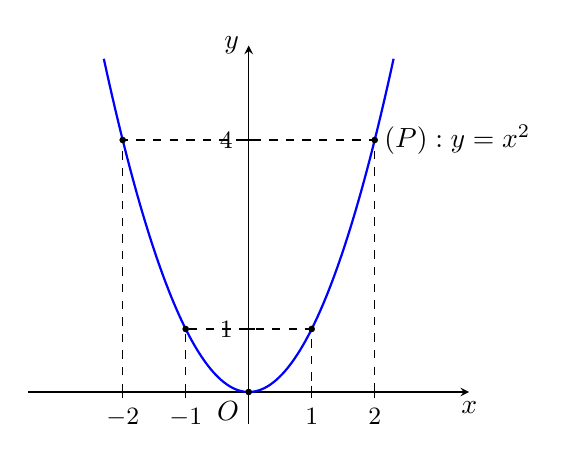
\begin{tikzpicture}[>=stealth, scale=0.8]
			\draw[->] (-3.5,0) -- (3.5,0) node[below] {$x$};
			\draw[->] (0,-0.5) -- (0,5.5) node[left] {$y$};
			\draw (0,0) node[below left] {$O$};
			\foreach \x in {-2,-1,1,2}
				\draw (\x,0.1) -- (\x,-0.1) node[below] {\small $\x$};
			\foreach \y in {1,4}
				\draw (0.1,\y) -- (-0.1,\y) node[left] {\small $\y$};
			\draw[dashed] (-2,0) -- (-2,4) -- (2,4) -- (2,0);
			\draw[dashed] (-1,0) -- (-1,1) -- (1,1) -- (1,0);
			\draw[smooth,samples=100,domain=-2.3:2.3,thick,blue] plot(\x,{(\x)^2});
			\node[right] at (2,4) {$(P): y=x^2$};
			\fill (-2,4) circle (1.5pt) (-1,1) circle (1.5pt) (0,0) circle (1.5pt) (1,1) circle (1.5pt) (2,4) circle (1.5pt);
		\end{tikzpicture}
		\end{center}
		\item Gọi điểm cần tìm là $M(x; y) \in (P)$.
		Theo đề bài, tung độ của điểm đó bằng $9$, tức là $y = 9$.
		Thay $y = 9$ vào phương trình parabol $(P)$, ta có:
		$$x^2 = 9 \iff x = 3 \text{ hoặc } x = -3.$$
		Vậy có hai điểm thuộc $(P)$ có tung độ bằng $9$ là $(3; 9)$ và $(-3; 9)$.
	\end{enumerate}
}
\end{bt}


\begin{bt}%[TS10 1.0 1.3]%[ma:dc255e41]
% nguon: Đề tham khảo Tuyển sinh 10 TP.HCM 2026-2027 – Cụm 1 (Đề 1), Bài 1, trang 3
Cho hàm số $(P): y = \dfrac{x^2}{4}$.
\begin{enumerate}[a)]
	\item Vẽ đồ thị $(P)$.
	\item Tìm điểm $K$ thuộc $(P)$ có tung độ nhỏ hơn hoành độ $1$ đơn vị.
\end{enumerate}
\loigiai{
\begin{enumerate}[a)]
		\item Bảng giá trị tương ứng giữa $x$ và $y$:
		\begin{center}
		\begin{tabular}{|c|c|c|c|c|c|}
		\hline
		$x$ & $-4$ & $-2$ & $0$ & $2$ & $4$ \\
		\hline
		$y = \dfrac{x^2}{4}$ & $4$ & $1$ & $0$ & $1$ & $4$ \\
		\hline
		\end{tabular}
		\end{center}
		Đồ thị $(P)$ là đường cong parabol đi qua gốc tọa độ $O(0; 0)$ và các điểm $(-4; 4)$, $(-2; 1)$, $(2; 1)$, $(4; 4)$, nhận trục tung $Oy$ làm trục đối xứng.
		\begin{center}
		\begin{tikzpicture}[>=stealth, scale=0.8]
			\draw[->] (-5,0) -- (5,0) node[below] {$x$};
			\draw[->] (0,-0.5) -- (0,5.5) node[left] {$y$};
			\draw (0,0) node[below left] {$O$};
			\foreach \x in {-4,-2,2,4}
				\draw (\x,0.1) -- (\x,-0.1) node[below] {\small $\x$};
			\foreach \y in {1,4}
				\draw (0.1,\y) -- (-0.1,\y) node[left] {\small $\y$};
			\draw[dashed] (-4,0) -- (-4,4) -- (4,4) -- (4,0);
			\draw[dashed] (-2,0) -- (-2,1) -- (2,1) -- (2,0);
			\draw[smooth,samples=100,domain=-4.4:4.4,thick,blue] plot(\x,{0.25*(\x)^2});
			\node[right] at (3.5,4.5) {$(P): y=\dfrac{x^2}{4}$};
			\fill (-4,4) circle (1.5pt) (-2,1) circle (1.5pt) (0,0) circle (1.5pt) (2,1) circle (1.5pt) (4,4) circle (1.5pt);
		\end{tikzpicture}
		\end{center}
		\item Gọi $K(x; y) \in (P)$. Vì điểm $K$ có tung độ nhỏ hơn hoành độ $1$ đơn vị nên:
		$$y = x - 1.$$
		Thay vào phương trình của parabol $(P)$, ta có:
		$$x - 1 = \frac{x^2}{4} \iff x^2 - 4x + 4 = 0 \iff (x - 2)^2 = 0 \iff x = 2.$$
		Với $x = 2$, suy ra $y = 2 - 1 = 1$.\\
		Vậy tọa độ điểm cần tìm là $K(2; 1)$.
	\end{enumerate}
}
\end{bt}

\begin{bt}%[TS10 1.0 1.2]%[ma:5f4b88a9]
% nguon: Đề tham khảo Tuyển sinh 10 TP.HCM 2026-2027 – Cụm 1 (Đề 2), Bài 1, trang 5
Cho hàm số $(P): y = -\dfrac{1}{2}x^2$.
\begin{enumerate}[a)]
	\item Vẽ đồ thị $(P)$.
	\item Tìm tọa độ điểm $M$ thuộc $(P)$ (khác gốc tọa độ) có hoành độ bằng $2$ lần tung độ.
\end{enumerate}
\loigiai{
\begin{enumerate}[a)]
		\item Bảng giá trị tương ứng giữa $x$ và $y$:
		\begin{center}
		\begin{tabular}{|c|c|c|c|c|c|}
		\hline
		$x$ & $-4$ & $-2$ & $0$ & $2$ & $4$ \\
		\hline
		$y = -\dfrac{1}{2}x^2$ & $-8$ & $-2$ & $0$ & $-2$ & $-8$ \\
		\hline
		\end{tabular}
		\end{center}
		Đồ thị $(P)$ là parabol đi qua gốc tọa độ $O(0; 0)$ và các điểm $(-4; -8)$, $(-2; -2)$, $(2; -2)$, $(4; -8)$, có bề lõm quay xuống dưới và nhận $Oy$ làm trục đối xứng.
		\begin{center}
		\begin{tikzpicture}[>=stealth, scale=0.7]
			\draw[->] (-5,0) -- (5,0) node[below] {$x$};
			\draw[->] (0,-9) -- (0,1.5) node[left] {$y$};
			\draw (0,0) node[above right] {$O$};
			\foreach \x in {-4,-2,2,4}
				\draw (\x,0.1) -- (\x,-0.1) node[above] {\small $\x$};
			\foreach \y in {-2,-8}
				\draw (0.1,\y) -- (-0.1,\y) node[left] {\small $\y$};
			\draw[dashed] (-4,0) -- (-4,-8) -- (4,-8) -- (4,0);
			\draw[dashed] (-2,0) -- (-2,-2) -- (2,-2) -- (2,0);
			\draw[smooth,samples=100,domain=-4.2:4.2,thick,blue] plot(\x,{-0.5*(\x)^2});
			\node[right] at (3.5,-4.5) {$(P): y=-\dfrac{1}{2}x^2$};
			\fill (-4,-8) circle (1.5pt) (-2,-2) circle (1.5pt) (0,0) circle (1.5pt) (2,-2) circle (1.5pt) (4,-8) circle (1.5pt);
		\end{tikzpicture}
		\end{center}
		\item Gọi $M(x; y) \in (P)$. Theo đề bài, hoành độ bằng $2$ lần tung độ nên:
		$$x = 2y \iff y = \frac{x}{2}.$$
		Thay vào phương trình của parabol $(P)$, ta có:
		$$\frac{x}{2} = -\frac{1}{2}x^2 \iff x^2 + x = 0 \iff x(x + 1) = 0 \iff \left[\begin{aligned} x &= 0 \\ x &= -1. \end{aligned}\right.$$
		Vì điểm $M$ khác gốc tọa độ $O(0; 0)$ nên $x = -1$.\\
		Với $x = -1$, suy ra $y = \dfrac{-1}{2} = -\dfrac{1}{2}$.\\
		Vậy tọa độ điểm cần tìm là $M\left(-1; -\dfrac{1}{2}\right)$.
	\end{enumerate}
}
\end{bt}


\begin{bt}%[TS10 1.0 1.1]%[ma:cfcce239]
% nguon: Đề tham khảo Tuyển sinh 10 TP.HCM 2026-2027 – Cụm 1 (Đề 3), Bài 1, trang 7
Cho hàm số $(P): y = x^2$.
\begin{enumerate}[a)]
	\item Vẽ đồ thị $(P)$.
	\item Tìm tọa độ các điểm $M$ thuộc $(P)$ có tung độ bằng $25$.
\end{enumerate}
\loigiai{
\begin{enumerate}[a)]
		\item Bảng giá trị tương ứng giữa $x$ và $y$:
		\begin{center}
		\begin{tabular}{|c|c|c|c|c|c|}
		\hline
		$x$ & $-2$ & $-1$ & $0$ & $1$ & $2$ \\
		\hline
		$y = x^2$ & $4$ & $1$ & $0$ & $1$ & $4$ \\
		\hline
		\end{tabular}
		\end{center}
		Đồ thị $(P)$ là đường cong parabol đi qua gốc tọa độ $O(0; 0)$ và các điểm $(-2; 4)$, $(-1; 1)$, $(1; 1)$, $(2; 4)$, nhận trục tung $Oy$ làm trục đối xứng và có bề lõm quay lên trên.
		\begin{center}
		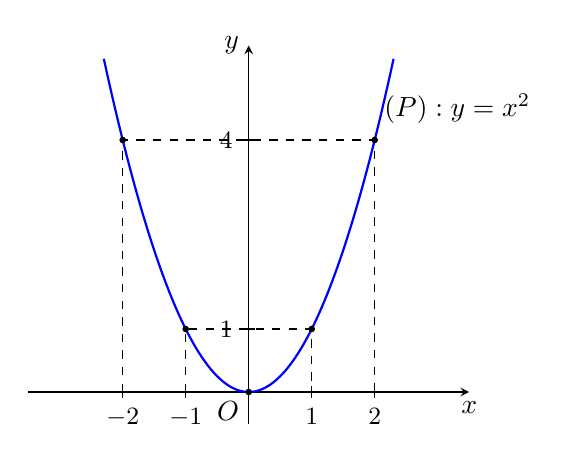
\begin{tikzpicture}[>=stealth, scale=0.8]
			\draw[->] (-3.5,0) -- (3.5,0) node[below] {$x$};
			\draw[->] (0,-0.5) -- (0,5.5) node[left] {$y$};
			\draw (0,0) node[below left] {$O$};
			\foreach \x in {-2,-1,1,2}
				\draw (\x,0.1) -- (\x,-0.1) node[below] {\small $\x$};
			\foreach \y in {1,4}
				\draw (0.1,\y) -- (-0.1,\y) node[left] {\small $\y$};
			\draw[dashed] (-2,0) -- (-2,4) -- (2,4) -- (2,0);
			\draw[dashed] (-1,0) -- (-1,1) -- (1,1) -- (1,0);
			\draw[smooth,samples=100,domain=-2.3:2.3,thick,blue] plot(\x,{(\x)^2});
			\node[right] at (2,4.5) {$(P): y=x^2$};
			\fill (-2,4) circle (1.5pt) (-1,1) circle (1.5pt) (0,0) circle (1.5pt) (1,1) circle (1.5pt) (2,4) circle (1.5pt);
		\end{tikzpicture}
		\end{center}
		\item Điểm $M(x; y) \in (P)$ có tung độ bằng $25$ nên $y = 25$.\\
		Thay $y = 25$ vào phương trình parabol $(P)$, ta có:
		$$x^2 = 25 \iff x^2 - 25 = 0 \iff x = 5 \text{ hoặc } x = -5.$$
		Với $x = 5 \implies y = 25$, ta được điểm $M_1(5; 25)$.\\
		Với $x = -5 \implies y = 25$, ta được điểm $M_2(-5; 25)$.\\
		Vậy có hai điểm thỏa mãn yêu cầu bài toán là $(5; 25)$ và $(-5; 25)$.
	\end{enumerate}
}
\end{bt}

\begin{bt}%[TS10 1.0 1.1]%[ma:693357d8]
% nguon: Đề tham khảo Tuyển sinh 10 TP.HCM 2026-2027 – Cụm 2 (Đề 1), Bài 1, trang 9
Cho hàm số $(P): y = \dfrac{3}{2}x^2$.
\begin{enumerate}[a)]
	\item Vẽ đồ thị $(P)$ trên hệ trục tọa độ.
	\item Tìm tọa độ các điểm thuộc $(P)$ có tung độ bằng $24$.
\end{enumerate}
\loigiai{
\begin{enumerate}[a)]
		\item Bảng giá trị tương ứng giữa $x$ và $y$:
		\begin{center}
		\begin{tabular}{|c|c|c|c|c|c|}
		\hline
		$x$ & $-2$ & $-1$ & $0$ & $1$ & $2$ \\
		\hline
		$y = \dfrac{3}{2}x^2$ & $6$ & $1{,}5$ & $0$ & $1{,}5$ & $6$ \\
		\hline
		\end{tabular}
		\end{center}
		Đồ thị $(P)$ là đường cong parabol đi qua gốc tọa độ $O(0; 0)$ và các điểm $(-2; 6)$, $(-1; 1{,}5)$, $(1; 1{,}5)$, $(2; 6)$, có bề lõm quay lên trên và nhận trục tung $Oy$ làm trục đối xứng.
		\begin{center}
		\begin{tikzpicture}[>=stealth, scale=0.8]
			\draw[->] (-3.5,0) -- (3.5,0) node[below] {$x$};
			\draw[->] (0,-0.5) -- (0,7) node[left] {$y$};
			\draw (0,0) node[below left] {$O$};
			\foreach \x in {-2,-1,1,2}
				\draw (\x,0.1) -- (\x,-0.1) node[below] {\small $\x$};
			\foreach \y in {1.5,6}
				\draw (0.1,\y) -- (-0.1,\y) node[left] {\small $\y$};
			\draw[dashed] (-2,0) -- (-2,6) -- (2,6) -- (2,0);
			\draw[dashed] (-1,0) -- (-1,1.5) -- (1,1.5) -- (1,0);
			\draw[smooth,samples=100,domain=-2.1:2.1,thick,blue] plot(\x,{1.5*(\x)^2});
			\node[right] at (1.8,6.5) {$(P): y=\dfrac{3}{2}x^2$};
			\fill (-2,6) circle (1.5pt) (-1,1.5) circle (1.5pt) (0,0) circle (1.5pt) (1,1.5) circle (1.5pt) (2,6) circle (1.5pt);
		\end{tikzpicture}
		\end{center}
		\item Gọi điểm cần tìm là $M(x; y) \in (P)$. Theo đề bài, tung độ của điểm đó bằng $24$, tức $y = 24$.\\
		Thay $y = 24$ vào phương trình parabol $(P)$, ta có:
		$$\frac{3}{2}x^2 = 24 \iff x^2 = 24 \cdot \frac{2}{3} = 16 \iff x = 4 \text{ hoặc } x = -4.$$
		Với $x = 4 \implies y = 24$, ta có điểm $M_1(4; 24)$.\\
		Với $x = -4 \implies y = 24$, ta có điểm $M_2(-4; 24)$.\\
		Vậy có hai điểm thuộc $(P)$ có tung độ bằng $24$ là $(4; 24)$ và $(-4; 24)$.
	\end{enumerate}
}
\end{bt}


\begin{bt}%[TS10 1.0 1.2]%[ma:64eec324]
% nguon: Đề tham khảo Tuyển sinh 10 TP.HCM 2026-2027 – Cụm 2 (Đề 2), Bài 1, trang 11
Cho hàm số $(P): y = \dfrac{1}{2}x^2$.
\begin{enumerate}[a)]
	\item Vẽ đồ thị $(P)$.
	\item Tìm điểm $M$ thuộc $(P)$ có tung độ gấp đôi hoành độ và khác gốc tọa độ.
\end{enumerate}
\loigiai{
\begin{enumerate}[a)]
		\item Bảng giá trị tương ứng giữa $x$ và $y$:
		\begin{center}
		\begin{tabular}{|c|c|c|c|c|c|}
		\hline
		$x$ & $-4$ & $-2$ & $0$ & $2$ & $4$ \\
		\hline
		$y = \dfrac{1}{2}x^2$ & $8$ & $2$ & $0$ & $2$ & $8$ \\
		\hline
		\end{tabular}
		\end{center}
		Đồ thị $(P)$ là đường cong parabol đi qua gốc tọa độ $O(0; 0)$ và các điểm $(-4; 8)$, $(-2; 2)$, $(2; 2)$, $(4; 8)$, nhận trục tung $Oy$ làm trục đối xứng và có bề lõm quay lên trên.
		\begin{center}
		\begin{tikzpicture}[>=stealth, scale=0.7]
			\draw[->] (-5,0) -- (5,0) node[below] {$x$};
			\draw[->] (0,-1) -- (0,9) node[left] {$y$};
			\draw (0,0) node[below left] {$O$};
			\foreach \x in {-4,-2,2,4}
				\draw (\x,0.1) -- (\x,-0.1) node[below] {\small $\x$};
			\foreach \y in {2,8}
				\draw (0.1,\y) -- (-0.1,\y) node[left] {\small $\y$};
			\draw[dashed] (-4,0) -- (-4,8) -- (4,8) -- (4,0);
			\draw[dashed] (-2,0) -- (-2,2) -- (2,2) -- (2,0);
			\draw[smooth,samples=100,domain=-4.2:4.2,thick,blue] plot(\x,{0.5*(\x)^2});
			\node[right] at (3.5,6.5) {$(P): y=\dfrac{1}{2}x^2$};
			\fill (-4,8) circle (1.5pt) (-2,2) circle (1.5pt) (0,0) circle (1.5pt) (2,2) circle (1.5pt) (4,8) circle (1.5pt);
		\end{tikzpicture}
		\end{center}
		\item Gọi $M(x; y) \in (P)$. Vì tung độ gấp đôi hoành độ nên:
		$$y = 2x.$$
		Thay vào phương trình parabol $(P)$, ta có:
		$$\frac{1}{2}x^2 = 2x \iff \frac{1}{2}x^2 - 2x = 0 \iff x\left(\frac{1}{2}x - 2\right) = 0 \iff \left[\begin{aligned} x &= 0 \\ x &= 4. \end{aligned}\right.$$
		Vì điểm $M$ khác gốc tọa độ $O(0; 0)$ nên ta nhận $x = 4$.\\
		Với $x = 4 \implies y = 2 \cdot 4 = 8$.\\
		Vậy tọa độ điểm cần tìm là $M(4; 8)$.
	\end{enumerate}
}
\end{bt}

\begin{bt}%[TS10 1.0 1.1]%[ma:132cec9b]
% nguon: Đề tham khảo Tuyển sinh 10 TP.HCM 2026-2027 – Cụm 2 (Đề 3), Bài 1, trang 13
Cho hàm số $(P): y = -\dfrac{1}{2}x^2$.
\begin{enumerate}[a)]
	\item Vẽ đồ thị $(P)$ của hàm số trên.
	\item Tìm những điểm $A$ thuộc $(P)$ sao cho tung độ bằng $-\dfrac{1}{2}$.
\end{enumerate}
\loigiai{
\begin{enumerate}[a)]
		\item Bảng giá trị tương ứng giữa $x$ và $y$:
		\begin{center}
		\begin{tabular}{|c|c|c|c|c|c|}
		\hline
		$x$ & $-4$ & $-2$ & $0$ & $2$ & $4$ \\
		\hline
		$y = -\dfrac{1}{2}x^2$ & $-8$ & $-2$ & $0$ & $-2$ & $-8$ \\
		\hline
		\end{tabular}
		\end{center}
		Đồ thị $(P)$ là đường cong parabol đi qua gốc tọa độ $O(0; 0)$ và các điểm $(-4; -8)$, $(-2; -2)$, $(2; -2)$, $(4; -8)$, nhận trục tung $Oy$ làm trục đối xứng và có bề lõm quay xuống dưới.
		\begin{center}
		\begin{tikzpicture}[>=stealth, scale=0.7]
			\draw[->] (-5,0) -- (5,0) node[below] {$x$};
			\draw[->] (0,-9) -- (0,1.5) node[left] {$y$};
			\draw (0,0) node[above right] {$O$};
			\foreach \x in {-4,-2,2,4}
				\draw (\x,0.1) -- (\x,-0.1) node[above] {\small $\x$};
			\foreach \y in {-2,-8}
				\draw (0.1,\y) -- (-0.1,\y) node[left] {\small $\y$};
			\draw[dashed] (-4,0) -- (-4,-8) -- (4,-8) -- (4,0);
			\draw[dashed] (-2,0) -- (-2,-2) -- (2,-2) -- (2,0);
			\draw[smooth,samples=100,domain=-4.2:4.2,thick,blue] plot(\x,{-0.5*(\x)^2});
			\node[right] at (3.5,-4.5) {$(P): y=-\dfrac{1}{2}x^2$};
			\fill (-4,-8) circle (1.5pt) (-2,-2) circle (1.5pt) (0,0) circle (1.5pt) (2,-2) circle (1.5pt) (4,-8) circle (1.5pt);
		\end{tikzpicture}
		\end{center}
		\item Điểm $A$ thuộc $(P)$ có tung độ bằng $-\dfrac{1}{2}$ nên $y = -\dfrac{1}{2}$.\\
		Thay $y = -\dfrac{1}{2}$ vào phương trình parabol $(P)$, ta có:
		$$-\frac{1}{2}x^2 = -\frac{1}{2} \iff x^2 = 1 \iff x = 1 \text{ hoặc } x = -1.$$
		Với $x = 1 \implies y = -\dfrac{1}{2}$, ta được điểm $A_1\left(1; -\dfrac{1}{2}\right)$.\\
		Với $x = -1 \implies y = -\dfrac{1}{2}$, ta được điểm $A_2\left(-1; -\dfrac{1}{2}\right)$.\\
		Vậy có hai điểm thỏa mãn yêu cầu là $\left(1; -\dfrac{1}{2}\right)$ và $\left(-1; -\dfrac{1}{2}\right)$.
	\end{enumerate}
}
\end{bt}


\begin{bt}%[TS10 1.0 1.2]%[ma:66192101]
% nguon: Đề tham khảo Tuyển sinh 10 năm học 2026-2027 Sở GD&ĐT TP.HCM - Cụm 3 Đề 1 - Bài 1
Cho hàm số $y = -\dfrac{1}{2}x^2$ có đồ thị là $(P)$.
\begin{enumerate}[a)]
	\item Vẽ đồ thị $(P)$ trên mặt phẳng tọa độ $Oxy$.
	\item Tìm tọa độ điểm $D$ thuộc $(P)$ ($D$ khác gốc tọa độ $O$) sao cho tung độ của điểm $D$ gấp đôi hoành độ của nó.
\end{enumerate}
\loigiai{
\begin{enumerate}[a)]
	\item Bảng giá trị của hàm số $y = -\dfrac{1}{2}x^2$:
	\begin{center}
		\begin{tabular}{|c|c|c|c|c|c|}
			\hline
			$x$ & $-4$ & $-2$ & $0$ & $2$ & $4$ \\ \hline
			$y$ & $-8$ & $-2$ & $0$ & $-2$ & $-8$ \\ \hline
		\end{tabular}
	\end{center}
	Đồ thị $(P)$ là một đường parabol đi qua các điểm $(-4; -8)$, $(-2; -2)$, $(0; 0)$, $(2; -2)$, $(4; -8)$, nhận trục $Oy$ làm trục đối xứng và có đỉnh là gốc tọa độ $O(0;0)$.
	\begin{center}
		\begin{tikzpicture}[>=stealth,scale=0.7]
			\draw[->] (-5,0) -- (5,0) node[below] {$x$};
			\draw[->] (0,-9) -- (0,1.5) node[left] {$y$};
			\draw (0,0) node[above right] {$O$};
			\foreach \x in {-4,-2,2,4}
				\draw (\x,0.1) -- (\x,-0.1) node[above] {\small $\x$};
			\foreach \y in {-8,-2}
				\draw (0.1,\y) -- (-0.1,\y) node[left] {\small $\y$};
			\draw[dashed] (-2,0) -- (-2,-2) -- (2,-2) -- (2,0);
			\draw[dashed] (-4,0) -- (-4,-8) -- (4,-8) -- (4,0);
			\draw[thick,smooth,samples=100,domain=-4.2:4.2] plot(\x,{-0.5*(\x)^2});
			\node[below right] at (2,-2) {$(P)$};
		\end{tikzpicture}
	\end{center}
	\item Gọi tọa độ điểm $D$ là $(x_D; y_D)$. Vì $D \in (P)$ nên $y_D = -\dfrac{1}{2}x_D^2$.\\
	Theo giả thiết, tung độ của $D$ gấp đôi hoành độ nên $y_D = 2x_D$.\\
	Ta có phương trình hoành độ giao điểm:
	$$-\dfrac{1}{2}x_D^2 = 2x_D \iff \dfrac{1}{2}x_D^2 + 2x_D = 0 \iff x_D\left(\dfrac{1}{2}x_D + 2\right) = 0 \iff \left[\begin{aligned} &x_D = 0 \\ &x_D = -4. \end{aligned}\right.$$
	Vì $D$ khác gốc tọa độ $O(0;0)$ nên $x_D = -4 \implies y_D = 2 \cdot (-4) = -8$.\\
	Vậy tọa độ điểm cần tìm là $D(-4; -8)$.
\end{enumerate}
}
\end{bt}

\begin{bt}%[TS10 1.0 1.1]%[ma:a512544e]
% nguon: Đề tham khảo Tuyển sinh 10 năm học 2026-2027 Sở GD&ĐT TP.HCM - Cụm 3 Đề 2 - Bài 1
Cho hàm số $y = \dfrac{x^2}{2}$ có đồ thị là parabol $(P)$.
\begin{enumerate}[a)]
	\item Vẽ đồ thị parabol $(P)$ trên mặt phẳng tọa độ $Oxy$.
	\item Tìm các điểm thuộc đồ thị $(P)$ có tung độ bằng $4$.
\end{enumerate}
\loigiai{
\begin{enumerate}[a)]
	\item Bảng giá trị của hàm số $y = \dfrac{x^2}{2}$:
	\begin{center}
		\begin{tabular}{|c|c|c|c|c|c|}
			\hline
			$x$ & $-4$ & $-2$ & $0$ & $2$ & $4$ \\ \hline
			$y$ & $8$ & $2$ & $0$ & $2$ & $8$ \\ \hline
		\end{tabular}
	\end{center}
	Đồ thị $(P)$ là một parabol đi qua các điểm $(-4; 8)$, $(-2; 2)$, $(0; 0)$, $(2; 2)$, $(4; 8)$, có đỉnh là gốc tọa độ $O(0;0)$ và nhận trục tung $Oy$ làm trục đối xứng.
	\begin{center}
		\begin{tikzpicture}[>=stealth,scale=0.7]
			\draw[->] (-5,0) -- (5,0) node[below] {$x$};
			\draw[->] (0,-1) -- (0,9) node[left] {$y$};
			\draw (0,0) node[below right] {$O$};
			\foreach \x in {-4,-2,2,4}
				\draw (\x,0.1) -- (\x,-0.1) node[below] {\small $\x$};
			\foreach \y in {2,4,8}
				\draw (0.1,\y) -- (-0.1,\y) node[left] {\small $\y$};
			\draw[dashed] (-2,0) -- (-2,2) -- (2,2) -- (2,0);
			\draw[dashed] (-4,0) -- (-4,8) -- (4,8) -- (4,0);
			\draw[thick,smooth,samples=100,domain=-4.1:4.1] plot(\x,{0.5*(\x)^2});
			\node[above left] at (2,2) {$(P)$};
		\end{tikzpicture}
	\end{center}
	\item Gọi điểm cần tìm là $N(x; y)$. Vì điểm $N$ thuộc đồ thị $(P)$ và có tung độ bằng $4$ nên:
	$$4 = \dfrac{x^2}{2} \iff x^2 = 8 \iff x = \pm 2\sqrt{2}.$$
	Vậy có hai điểm thỏa mãn yêu cầu bài toán là $(2\sqrt{2}; 4)$ và $(-2\sqrt{2}; 4)$.
\end{enumerate}
}
\end{bt}


\begin{bt}%[TS10 1.0 1.2]%[ma:38d7a768]
% nguon: Đề tham khảo Tuyển sinh 10 năm học 2026-2027 Sở GD&ĐT TP.HCM - Cụm 3 Đề 3 - Bài 1
Cho hàm số $y = -\dfrac{1}{2}x^2$ có đồ thị là parabol $(P)$.
\begin{enumerate}[a)]
	\item Vẽ đồ thị $(P)$ trên mặt phẳng tọa độ $Oxy$.
	\item Tìm những điểm thuộc đồ thị $(P)$ có hoành độ gấp hai lần tung độ.
\end{enumerate}
\loigiai{
\begin{enumerate}[a)]
	\item Bảng giá trị của hàm số $y = -\dfrac{1}{2}x^2$:
	\begin{center}
		\begin{tabular}{|c|c|c|c|c|c|}
			\hline
			$x$ & $-4$ & $-2$ & $0$ & $2$ & $4$ \\ \hline
			$y$ & $-8$ & $-2$ & $0$ & $-2$ & $-8$ \\ \hline
		\end{tabular}
	\end{center}
	Đồ thị $(P)$ là một parabol đi qua các điểm $(-4; -8)$, $(-2; -2)$, $(0; 0)$, $(2; -2)$, $(4; -8)$, nhận trục tung $Oy$ làm trục đối xứng và có đỉnh là gốc tọa độ $O(0;0)$.
	\begin{center}
		\begin{tikzpicture}[>=stealth,scale=0.7]
			\draw[->] (-5,0) -- (5,0) node[below] {$x$};
			\draw[->] (0,-9) -- (0,1.5) node[left] {$y$};
			\draw (0,0) node[above right] {$O$};
			\foreach \x in {-4,-2,2,4}
				\draw (\x,0.1) -- (\x,-0.1) node[above] {\small $\x$};
			\foreach \y in {-8,-2}
				\draw (0.1,\y) -- (-0.1,\y) node[left] {\small $\y$};
			\draw[dashed] (-2,0) -- (-2,-2) -- (2,-2) -- (2,0);
			\draw[dashed] (-4,0) -- (-4,-8) -- (4,-8) -- (4,0);
			\draw[thick,smooth,samples=100,domain=-4.2:4.2] plot(\x,{-0.5*(\x)^2});
			\node[below right] at (2,-2) {$(P)$};
		\end{tikzpicture}
	\end{center}
	\item Gọi $M(x; y)$ là điểm thuộc đồ thị $(P)$ có hoành độ gấp hai lần tung độ.\\
	Ta có $x = 2y \implies y = \dfrac{1}{2}x$.\\
	Vì $M \in (P)$ nên ta có phương trình hoành độ giao điểm:
	$$\dfrac{1}{2}x = -\dfrac{1}{2}x^2 \iff \dfrac{1}{2}x^2 + \dfrac{1}{2}x = 0 \iff \dfrac{1}{2}x(x + 1) = 0 \iff \left[\begin{aligned} &x = 0 \\ &x = -1. \end{aligned}\right.$$
	\begin{itemize}
		\item Với $x = 0 \implies y = 0$, ta được điểm $O(0; 0)$.
		\item Với $x = -1 \implies y = -\dfrac{1}{2}$, ta được điểm $\left(-1; -\dfrac{1}{2}\right)$.
	\end{itemize}
	Vậy tọa độ các điểm cần tìm là $(0; 0)$ và $\left(-1; -\dfrac{1}{2}\right)$.
\end{enumerate}
}
\end{bt}

\begin{bt}%[TS10 1.0 1.2]%[ma:03980d37]
% nguon: Đề tham khảo Tuyển sinh 10 năm học 2026-2027 Sở GD&ĐT TP.HCM - Cụm 4 Đề 1 - Bài 1
Cho hàm số $y = \dfrac{1}{2}x^2$ có đồ thị là parabol $(P)$.
\begin{enumerate}[a)]
	\item Vẽ đồ thị parabol $(P)$ trên mặt phẳng tọa độ $Oxy$.
	\item Tìm tọa độ điểm $M$ thuộc đồ thị $(P)$ ($M$ khác gốc tọa độ $O$) có tung độ gấp đôi hoành độ.
\end{enumerate}
\loigiai{
\begin{enumerate}[a)]
	\item Bảng giá trị của hàm số $y = \dfrac{1}{2}x^2$:
	\begin{center}
		\begin{tabular}{|c|c|c|c|c|c|}
			\hline
			$x$ & $-2$ & $-1$ & $0$ & $1$ & $2$ \\ \hline
			$y$ & $2$ & $0{,}5$ & $0$ & $0{,}5$ & $2$ \\ \hline
		\end{tabular}
	\end{center}
	Đồ thị $(P)$ là một parabol đi qua các điểm $(-2; 2)$, $(-1; 0{,}5)$, $(0; 0)$, $(1; 0{,}5)$, $(2; 2)$, có đỉnh là gốc tọa độ $O(0;0)$ và nhận trục tung $Oy$ làm trục đối xứng.
	\begin{center}
		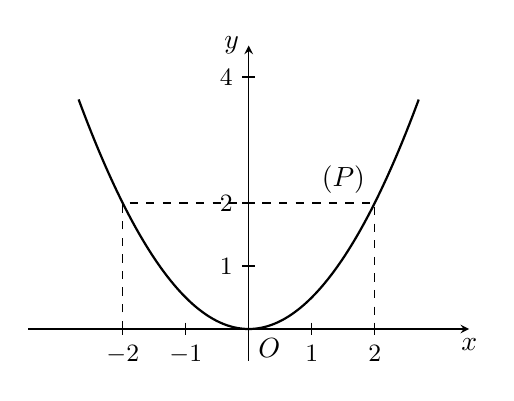
\begin{tikzpicture}[>=stealth,scale=0.8]
			\draw[->] (-3.5,0) -- (3.5,0) node[below] {$x$};
			\draw[->] (0,-0.5) -- (0,4.5) node[left] {$y$};
			\draw (0,0) node[below right] {$O$};
			\foreach \x in {-2,-1,1,2}
				\draw (\x,0.1) -- (\x,-0.1) node[below] {\small $\x$};
			\foreach \y in {1,2,4}
				\draw (0.1,\y) -- (-0.1,\y) node[left] {\small $\y$};
			\draw[dashed] (-2,0) -- (-2,2) -- (2,2) -- (2,0);
			\draw[thick,smooth,samples=100,domain=-2.7:2.7] plot(\x,{0.5*(\x)^2});
			\node[above left] at (2,2) {$(P)$};
		\end{tikzpicture}
	\end{center}
	\item Gọi điểm cần tìm là $M(x; y)$. Vì điểm $M$ có tung độ gấp đôi hoành độ nên $y = 2x$.\\
	Vì $M \in (P)$ nên ta có phương trình:
	$$\dfrac{1}{2}x^2 = 2x \iff \dfrac{1}{2}x^2 - 2x = 0 \iff x\left(\dfrac{1}{2}x - 2\right) = 0 \iff \left[\begin{aligned} &x = 0 \\ &x = 4. \end{aligned}\right.$$
	Vì điểm $M$ khác gốc tọa độ $O(0; 0)$ nên chọn $x = 4 \implies y = 2 \cdot 4 = 8$.\\
	Vậy tọa độ điểm cần tìm là $M(4; 8)$.
\end{enumerate}
}
\end{bt}


\begin{bt}%[TS10 1.0 1.2]%[ma:cfb4fcdd]
% nguon: Đề tham khảo Tuyển sinh 10 năm học 2026-2027 Sở GD&ĐT TP.HCM - Cụm 4 Đề 2 - Bài 1
Cho hàm số $y = \dfrac{x^2}{2}$ có đồ thị là Parabol $(P)$.
\begin{enumerate}[a)]
	\item Vẽ đồ thị $(P)$ trên mặt phẳng tọa độ $Oxy$.
	\item Tìm tọa độ các điểm thuộc $(P)$ có tung độ gấp đôi hoành độ.
\end{enumerate}
\loigiai{
\begin{enumerate}[a)]
	\item Bảng giá trị của hàm số $y = \dfrac{x^2}{2}$:
	\begin{center}
		\begin{tabular}{|c|c|c|c|c|c|}
			\hline
			$x$ & $-4$ & $-2$ & $0$ & $2$ & $4$ \\ \hline
			$y$ & $8$ & $2$ & $0$ & $2$ & $8$ \\ \hline
		\end{tabular}
	\end{center}
	Đồ thị $(P)$ là một đường parabol đi qua các điểm $(-4; 8)$, $(-2; 2)$, $(0; 0)$, $(2; 2)$, $(4; 8)$, nhận trục tung $Oy$ làm trục đối xứng và có đỉnh là gốc tọa độ $O(0;0)$.
	\begin{center}
		\begin{tikzpicture}[>=stealth,scale=0.7]
			\draw[->] (-5,0) -- (5,0) node[below] {$x$};
			\draw[->] (0,-1) -- (0,9) node[left] {$y$};
			\draw (0,0) node[below right] {$O$};
			\foreach \x in {-4,-2,2,4}
				\draw (\x,0.1) -- (\x,-0.1) node[below] {\small $\x$};
			\foreach \y in {2,8}
				\draw (0.1,\y) -- (-0.1,\y) node[left] {\small $\y$};
			\draw[dashed] (-2,0) -- (-2,2) -- (2,2) -- (2,0);
			\draw[dashed] (-4,0) -- (-4,8) -- (4,8) -- (4,0);
			\draw[thick,smooth,samples=100,domain=-4.1:4.1] plot(\x,{0.5*(\x)^2});
			\node[above left] at (2,2) {$(P)$};
		\end{tikzpicture}
	\end{center}
	\item Gọi điểm cần tìm là $M(x; y)$. Vì điểm $M$ thuộc $(P)$ và có tung độ gấp đôi hoành độ nên $y = 2x$.\\
	Ta có phương trình hoành độ giao điểm:
	$$\dfrac{x^2}{2} = 2x \iff \dfrac{x^2}{2} - 2x = 0 \iff x\left(\dfrac{x}{2} - 2\right) = 0 \iff \left[\begin{aligned} &x = 0 \\ &x = 4. \end{aligned}\right.$$
	\begin{itemize}
		\item Với $x = 0 \implies y = 0$, ta được điểm $O(0; 0)$.
		\item Với $x = 4 \implies y = 2 \cdot 4 = 8$, ta được điểm $A(4; 8)$.
	\end{itemize}
	Vậy tọa độ các điểm cần tìm là $(0; 0)$ và $(4; 8)$.
\end{enumerate}
}
\end{bt}

\begin{bt}%[TS10 1.0 1.2]%[ma:9527a3e2]
% nguon: Đề tham khảo Tuyển sinh 10 năm học 2026-2027 Sở GD&ĐT TP.HCM - Cụm 4 Đề 3 - Bài 1
Cho hàm số $y = -\dfrac{x^2}{4}$ có đồ thị là Parabol $(P)$.
\begin{enumerate}[a)]
	\item Vẽ đồ thị $(P)$ của hàm số trên mặt phẳng tọa độ $Oxy$.
	\item Tìm tọa độ các điểm $M$ thuộc đồ thị $(P)$ có tung độ bằng $2$ lần hoành độ.
\end{enumerate}
\loigiai{
\begin{enumerate}[a)]
	\item Bảng giá trị của hàm số $y = -\dfrac{x^2}{4}$:
	\begin{center}
		\begin{tabular}{|c|c|c|c|c|c|}
			\hline
			$x$ & $-4$ & $-2$ & $0$ & $2$ & $4$ \\ \hline
			$y$ & $-4$ & $-1$ & $0$ & $-1$ & $-4$ \\ \hline
		\end{tabular}
	\end{center}
	Đồ thị $(P)$ là một parabol đi qua các điểm $(-4; -4)$, $(-2; -1)$, $(0; 0)$, $(2; -1)$, $(4; -4)$, có đỉnh là gốc tọa độ $O(0;0)$ và nhận trục tung $Oy$ làm trục đối xứng.
	\begin{center}
		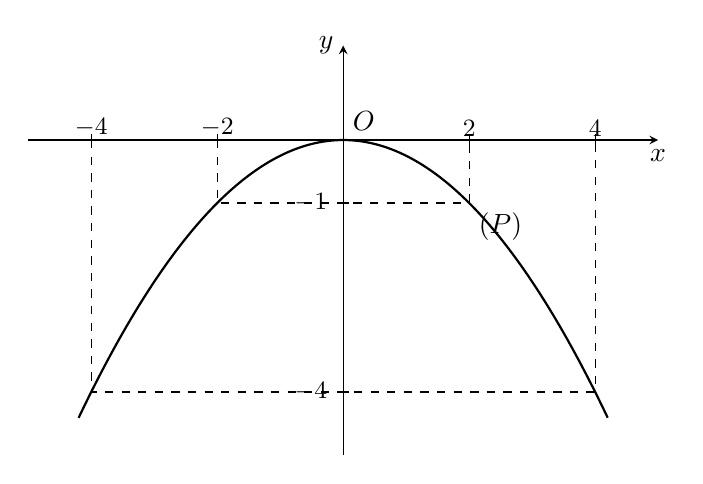
\begin{tikzpicture}[>=stealth,scale=0.8]
			\draw[->] (-5,0) -- (5,0) node[below] {$x$};
			\draw[->] (0,-5) -- (0,1.5) node[left] {$y$};
			\draw (0,0) node[above right] {$O$};
			\foreach \x in {-4,-2,2,4}
				\draw (\x,0.1) -- (\x,-0.1) node[above] {\small $\x$};
			\foreach \y in {-4,-1}
				\draw (0.1,\y) -- (-0.1,\y) node[left] {\small $\y$};
			\draw[dashed] (-2,0) -- (-2,-1) -- (2,-1) -- (2,0);
			\draw[dashed] (-4,0) -- (-4,-4) -- (4,-4) -- (4,0);
			\draw[thick,smooth,samples=100,domain=-4.2:4.2] plot(\x,{-0.25*(\x)^2});
			\node[below right] at (2,-1) {$(P)$};
		\end{tikzpicture}
	\end{center}
	\item Vì điểm $M$ thuộc $(P)$ có tung độ bằng $2$ lần hoành độ nên ta có $y = 2x$.\\
	Phương trình hoành độ giao điểm là:
	$$2x = -\dfrac{x^2}{4} \iff \dfrac{x^2}{4} + 2x = 0 \iff x\left(\dfrac{x}{4} + 2\right) = 0 \iff \left[\begin{aligned} &x = 0 \\ &x = -8. \end{aligned}\right.$$
	\begin{itemize}
		\item Với $x = 0 \implies y = 0$, ta được điểm $O(0; 0)$.
		\item Với $x = -8 \implies y = 2 \cdot (-8) = -16$, ta được điểm $M(-8; -16)$.
	\end{itemize}
	Vậy tọa độ các điểm cần tìm là $(0; 0)$ và $(-8; -16)$.
\end{enumerate}
}
\end{bt}


\begin{bt}%[TS10 1.0 1.1]%[ma:e6051d82]
% nguon: Đề tham khảo Tuyển sinh 10 năm học 2026-2027 Sở GD&ĐT TP.HCM - Cụm 5 Đề 1 - Bài 1
Cho hàm số $y = 2x^2$ có đồ thị $(P)$.
\begin{enumerate}[a)]
	\item Vẽ đồ thị $(P)$ trên hệ trục tọa độ $Oxy$.
	\item Tìm tọa độ các điểm thuộc $(P)$ có tung độ bằng $16$.
\end{enumerate}
\loigiai{
\begin{enumerate}[a)]
	\item Bảng giá trị của hàm số $y = 2x^2$:
	\begin{center}
		\begin{tabular}{|c|c|c|c|c|c|}
			\hline
			$x$ & $-2$ & $-1$ & $0$ & $1$ & $2$ \\ \hline
			$y$ & $8$ & $2$ & $0$ & $2$ & $8$ \\ \hline
		\end{tabular}
	\end{center}
	Đồ thị $(P)$ là một parabol đi qua các điểm $(-2; 8)$, $(-1; 2)$, $(0; 0)$, $(1; 2)$, $(2; 8)$, nhận trục tung $Oy$ làm trục đối xứng và có đỉnh là gốc tọa độ $O(0;0)$.
	\begin{center}
		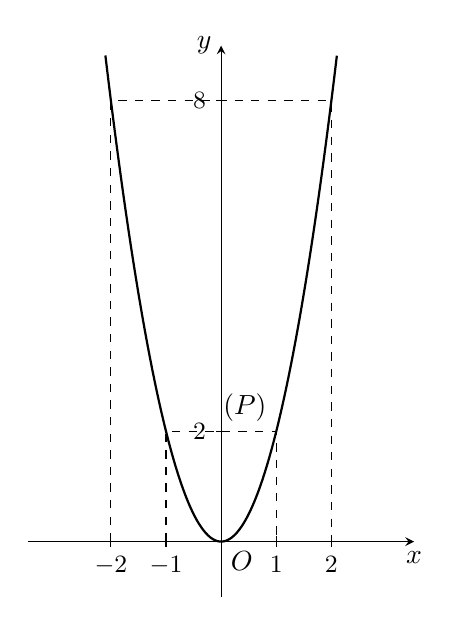
\begin{tikzpicture}[>=stealth,scale=0.7]
			\draw[->] (-3.5,0) -- (3.5,0) node[below] {$x$};
			\draw[->] (0,-1) -- (0,9) node[left] {$y$};
			\draw (0,0) node[below right] {$O$};
			\foreach \x in {-2,-1,1,2}
				\draw (\x,0.1) -- (\x,-0.1) node[below] {\small $\x$};
			\foreach \y in {2,8}
				\draw (0.1,\y) -- (-0.1,\y) node[left] {\small $\y$};
			\draw[dashed] (-1,0) -- (-1,2) -- (1,2) -- (1,0);
			\draw[dashed] (-2,0) -- (-2,8) -- (2,8) -- (2,0);
			\draw[thick,smooth,samples=100,domain=-2.1:2.1] plot(\x,{2*(\x)^2});
			\node[above left] at (1,2) {$(P)$};
		\end{tikzpicture}
	\end{center}
	\item Gọi điểm cần tìm là $N(x; y)$. Vì điểm $N$ thuộc $(P)$ và có tung độ bằng $16$ nên:
	$$2x^2 = 16 \iff x^2 = 8 \iff x = \pm 2\sqrt{2}.$$
	Vậy có hai điểm thỏa mãn yêu cầu là $(2\sqrt{2}; 16)$ và $(-2\sqrt{2}; 16)$.
\end{enumerate}
}
\end{bt}

\begin{bt}%[TS10 1.0 1.2]%[ma:83fb2473]
% nguon: Đề tham khảo Tuyển sinh 10 năm học 2026-2027 Sở GD&ĐT TP.HCM - Cụm 5 Đề 2 - Bài 1
Cho hàm số $y = x^2$ có đồ thị là Parabol $(P)$.
\begin{enumerate}[a)]
	\item Vẽ đồ thị $(P)$ của hàm số trên mặt phẳng tọa độ $Oxy$.
	\item Tìm tọa độ những điểm $M$ thuộc $(P)$ có tung độ bằng hai lần hoành độ bằng phép tính.
\end{enumerate}
\loigiai{
\begin{enumerate}[a)]
	\item Bảng giá trị của hàm số $y = x^2$:
	\begin{center}
		\begin{tabular}{|c|c|c|c|c|c|}
			\hline
			$x$ & $-2$ & $-1$ & $0$ & $1$ & $2$ \\ \hline
			$y$ & $4$ & $1$ & $0$ & $1$ & $4$ \\ \hline
		\end{tabular}
	\end{center}
	Đồ thị $(P)$ là một parabol đi qua các điểm $(-2; 4)$, $(-1; 1)$, $(0; 0)$, $(1; 1)$, $(2; 4)$, nhận trục tung $Oy$ làm trục đối xứng và có đỉnh là gốc tọa độ $O(0;0)$.
	\begin{center}
		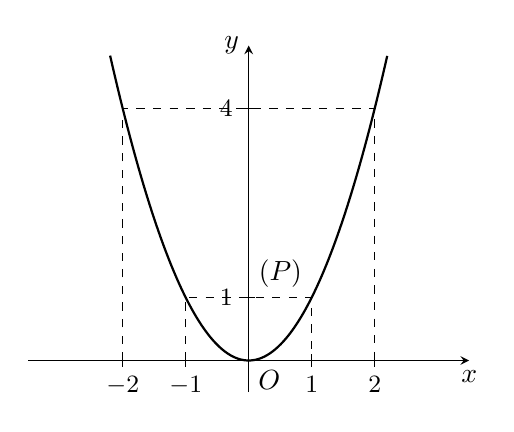
\begin{tikzpicture}[>=stealth,scale=0.8]
			\draw[->] (-3.5,0) -- (3.5,0) node[below] {$x$};
			\draw[->] (0,-0.5) -- (0,5) node[left] {$y$};
			\draw (0,0) node[below right] {$O$};
			\foreach \x in {-2,-1,1,2}
				\draw (\x,0.1) -- (\x,-0.1) node[below] {\small $\x$};
			\foreach \y in {1,4}
				\draw (0.1,\y) -- (-0.1,\y) node[left] {\small $\y$};
			\draw[dashed] (-1,0) -- (-1,1) -- (1,1) -- (1,0);
			\draw[dashed] (-2,0) -- (-2,4) -- (2,4) -- (2,0);
			\draw[thick,smooth,samples=100,domain=-2.2:2.2] plot(\x,{(\x)^2});
			\node[above left] at (1,1) {$(P)$};
		\end{tikzpicture}
	\end{center}
	\item Điểm $M$ thuộc $(P)$ có tung độ bằng hai lần hoành độ nên ta có $y = 2x$.\\
	Phương trình hoành độ giao điểm là:
	$$x^2 = 2x \iff x^2 - 2x = 0 \iff x(x - 2) = 0 \iff \left[\begin{aligned} &x = 0 \\ &x = 2. \end{aligned}\right.$$
	\begin{itemize}
		\item Với $x = 0 \implies y = 0$, ta được điểm $O(0; 0)$.
		\item Với $x = 2 \implies y = 2 \cdot 2 = 4$, ta được điểm $M(2; 4)$.
	\end{itemize}
	Vậy tọa độ các điểm cần tìm là $(0; 0)$ và $(2; 4)$.
\end{enumerate}
}
\end{bt}


\begin{bt}%[TS10 1.0 1.2]%[ma:ffae39a3]
% nguon: Đề tham khảo Tuyển sinh 10 năm học 2026-2027 Sở GD&ĐT TP.HCM - Cụm 6 Đề 1, Bài 1
Cho parabol $(P)\colon y = -\dfrac{1}{3}x^2$.
	\begin{enumerate}[a)]
		\item Vẽ đồ thị $(P)$.
		\item Tìm các điểm $N$ thuộc $(P)$ (khác gốc tọa độ $O$) sao cho tung độ gấp $3$ lần hoành độ.
	\end{enumerate}
\loigiai{
\begin{enumerate}[a)]
			\item Bảng giá trị tương ứng giữa $x$ và $y$ của parabol $(P)\colon y = -\dfrac{1}{3}x^2$:
			\begin{center}
				\begin{tabular}{|c|c|c|c|c|c|}
					\hline
					$x$ & $-6$ & $-3$ & $0$ & $3$ & $6$ \\
					\hline
					$y = -\dfrac{1}{3}x^2$ & $-12$ & $-3$ & $0$ & $-3$ & $-12$ \\
					\hline
				\end{tabular}
			\end{center}
			Đồ thị $(P)$ là một parabol đi qua gốc tọa độ $O(0;0)$ và nhận trục tung $Oy$ làm trục đối xứng.
			\begin{center}
				\begin{tikzpicture}[>=stealth, scale=0.6]
					\draw[->] (-7,0) -- (7,0) node[below] {$x$};
					\draw[->] (0,-13) -- (0,2) node[left] {$y$};
					\fill (0,0) circle (1.5pt) node[above right] {$O$};
					\draw[smooth, samples=100, domain=-6.2:6.2, thick, color=blue] plot(\x, {-1/3*(\x)^2});
					\draw[dashed] (-3,0) node[above] {$-3$} -- (-3,-3) -- (0,-3) node[right] {$-3$} -- (3,-3) -- (3,0) node[above] {$3$};
					\draw[dashed] (-6,0) node[above] {$-6$} -- (-6,-12) -- (0,-12) node[right] {$-12$} -- (6,-12) -- (6,0) node[above] {$6$};
					\fill (-3,-3) circle (1.5pt) (3,-3) circle (1.5pt) (-6,-12) circle (1.5pt) (6,-12) circle (1.5pt);
				\end{tikzpicture}
			\end{center}
			\item Gọi tọa độ điểm $N(x_N; y_N) \in (P)$.
			
			Vì tung độ gấp $3$ lần hoành độ nên $y_N = 3x_N$.
			
			Mặt khác, $N \in (P)$ nên $y_N = -\dfrac{1}{3}x_N^2$. Do đó:
			$$-\dfrac{1}{3}x_N^2 = 3x_N \iff x_N^2 + 9x_N = 0 \iff x_N(x_N + 9) = 0 \iff \left[\begin{aligned} &x_N = 0 \\ &x_N = -9. \end{aligned}\right.$$
			Vì $N \neq O$ nên $x_N \neq 0$, suy ra $x_N = -9$.
			
			Với $x_N = -9 \implies y_N = 3 \cdot (-9) = -27$.
			
			Vậy tọa độ điểm cần tìm là $N(-9; -27)$.
		\end{enumerate}
}
\end{bt}

\begin{bt}%[TS10 1.0 1.1]%[ma:b912366c]
% nguon: Đề tham khảo Tuyển sinh 10 năm học 2026-2027 Sở GD&ĐT TP.HCM - Cụm 6 Đề 2, Bài 1
Cho hàm số $y = x^2$ có đồ thị là parabol $(P)$.
	\begin{enumerate}[a)]
		\item Vẽ đồ thị $(P)$.
		\item Tìm tọa độ các điểm thuộc $(P)$ có tung độ bằng $12$.
	\end{enumerate}
\loigiai{
\begin{enumerate}[a)]
			\item Bảng giá trị của hàm số $y = x^2$:
			\begin{center}
				\begin{tabular}{|c|c|c|c|c|c|}
					\hline
					$x$ & $-2$ & $-1$ & $0$ & $1$ & $2$ \\
					\hline
					$y = x^2$ & $4$ & $1$ & $0$ & $1$ & $4$ \\
					\hline
				\end{tabular}
			\end{center}
			Đồ thị $(P)$ là đường parabol đi qua gốc tọa độ $O(0;0)$, nằm phía trên trục hoành và nhận trục tung $Oy$ làm trục đối xứng.
			\begin{center}
				\begin{tikzpicture}[>=stealth, scale=0.7]
					\draw[->] (-3.5,0) -- (3.5,0) node[below] {$x$};
					\draw[->] (0,-1) -- (0,5.5) node[left] {$y$};
					\fill (0,0) circle (1.5pt) node[below right] {$O$};
					\draw[smooth, samples=100, domain=-2.3:2.3, thick, color=blue] plot(\x, {(\x)^2});
					\draw[dashed] (-2,0) node[below] {$-2$} -- (-2,4) -- (0,4) node[left] {$4$} -- (2,4) -- (2,0) node[below] {$2$};
					\draw[dashed] (-1,0) node[below] {$-1$} -- (-1,1) -- (0,1) node[right] {$1$} -- (1,1) -- (1,0) node[below] {$1$};
					\fill (-2,4) circle (1.5pt) (2,4) circle (1.5pt) (-1,1) circle (1.5pt) (1,1) circle (1.5pt);
				\end{tikzpicture}
			\end{center}
			\item Điểm thuộc $(P)$ có tung độ bằng $12$ nên $y = 12$.
			
			Thay $y = 12$ vào phương trình parabol $(P)$, ta được:
			$$x^2 = 12 \iff x = \pm \sqrt{12} = \pm 2\sqrt{3}.$$
			Vậy có hai điểm thỏa mãn yêu cầu đề bài là $(2\sqrt{3}; 12)$ và $(-2\sqrt{3}; 12)$.
		\end{enumerate}
}
\end{bt}


\begin{bt}%[TS10 1.0 1.2]%[ma:67e7a0cc]
% nguon: Đề tham khảo Tuyển sinh 10 năm học 2026-2027 Sở GD&ĐT TP.HCM - Cụm 6 Đề 3, Bài 1
Cho hàm số $(P)\colon y = \dfrac{2}{3}x^2$.
	\begin{enumerate}[a)]
		\item Vẽ đồ thị $(P)$ trên mặt phẳng tọa độ $Oxy$.
		\item Tìm điểm thuộc $(P)$ sao cho hoành độ khác $0$ và gấp $2$ lần tung độ.
	\end{enumerate}
\loigiai{
\begin{enumerate}[a)]
			\item Bảng giá trị tương ứng giữa $x$ và $y$ của parabol $(P)\colon y = \dfrac{2}{3}x^2$:
			\begin{center}
				\begin{tabular}{|c|c|c|c|c|c|}
					\hline
					$x$ & $-3$ & $-1{,}5$ & $0$ & $1{,}5$ & $3$ \\
					\hline
					$y = \dfrac{2}{3}x^2$ & $6$ & $1{,}5$ & $0$ & $1{,}5$ & $6$ \\
					\hline
				\end{tabular}
			\end{center}
			Đồ thị $(P)$ là một parabol đi qua gốc tọa độ $O(0;0)$, nằm phía trên trục hoành và nhận trục tung $Oy$ làm trục đối xứng.
			\begin{center}
				\begin{tikzpicture}[>=stealth, scale=0.7]
					\draw[->] (-4,0) -- (4,0) node[below] {$x$};
					\draw[->] (0,-1) -- (0,7) node[left] {$y$};
					\fill (0,0) circle (1.5pt) node[below right] {$O$};
					\draw[smooth, samples=100, domain=-3.1:3.1, thick, color=blue] plot(\x, {2/3*(\x)^2});
					\draw[dashed] (-3,0) node[below] {$-3$} -- (-3,6) -- (0,6) node[left] {$6$} -- (3,6) -- (3,0) node[below] {$3$};
					\draw[dashed] (-1.5,0) node[below] {$-1{,}5$} -- (-1.5,1.5) -- (0,1.5) node[left] {$1{,}5$} -- (1.5,1.5) -- (1.5,0) node[below] {$1{,}5$};
					\fill (-3,6) circle (1.5pt) (3,6) circle (1.5pt) (-1.5,1.5) circle (1.5pt) (1.5,1.5) circle (1.5pt);
				\end{tikzpicture}
			\end{center}
			\item Gọi tọa độ điểm cần tìm là $M(x; y) \in (P)$.
			
			Vì hoành độ gấp $2$ lần tung độ nên $x = 2y \iff y = \dfrac{1}{2}x$.
			
			Mặt khác $M \in (P)$ nên ta có phương trình:
			$$\dfrac{2}{3}x^2 = \dfrac{1}{2}x \iff \dfrac{2}{3}x^2 - \dfrac{1}{2}x = 0 \iff x\left(\dfrac{2}{3}x - \dfrac{1}{2}\right) = 0 \iff \left[\begin{aligned} &x = 0 \\ &x = \dfrac{3}{4}. \end{aligned}\right.$$
			Vì hoành độ khác $0$ nên $x = \dfrac{3}{4}$.
			
			Với $x = \dfrac{3}{4} \implies y = \dfrac{1}{2} \cdot \dfrac{3}{4} = \dfrac{3}{8}$.
			
			Vậy tọa độ điểm cần tìm là $\left(\dfrac{3}{4}; \dfrac{3}{8}\right)$.
		\end{enumerate}
}
\end{bt}

\begin{bt}%[TS10 1.0 1.2]%[ma:4cf6579a]
% nguon: Đề tham khảo Tuyển sinh 10 năm học 2026-2027 Sở GD&ĐT TP.HCM - Cụm 7 Đề 1, Bài 1
Cho hàm số $(P)\colon y = \dfrac{1}{2}x^2$.
	\begin{enumerate}[a)]
		\item Vẽ đồ thị $(P)$ của hàm số trên mặt phẳng tọa độ $Oxy$.
		\item Tìm điểm $A$ (khác gốc tọa độ $O$) thuộc $(P)$ có tung độ gấp đôi hoành độ.
	\end{enumerate}
\loigiai{
\begin{enumerate}[a)]
			\item Bảng giá trị tương ứng giữa $x$ và $y$ của parabol $(P)\colon y = \dfrac{1}{2}x^2$:
			\begin{center}
				\begin{tabular}{|c|c|c|c|c|c|}
					\hline
					$x$ & $-4$ & $-2$ & $0$ & $2$ & $4$ \\
					\hline
					$y = \dfrac{1}{2}x^2$ & $8$ & $2$ & $0$ & $2$ & $8$ \\
					\hline
				\end{tabular}
			\end{center}
			Đồ thị $(P)$ là một parabol đi qua gốc tọa độ $O(0;0)$, nằm phía trên trục hoành và nhận trục tung $Oy$ làm trục đối xứng.
			\begin{center}
				\begin{tikzpicture}[>=stealth, scale=0.7]
					\draw[->] (-5,0) -- (5,0) node[below] {$x$};
					\draw[->] (0,-1) -- (0,9) node[left] {$y$};
					\fill (0,0) circle (1.5pt) node[below right] {$O$};
					\draw[smooth, samples=100, domain=-4.2:4.2, thick, color=blue] plot(\x, {1/2*(\x)^2});
					\draw[dashed] (-4,0) node[below] {$-4$} -- (-4,8) -- (0,8) node[left] {$8$} -- (4,8) -- (4,0) node[below] {$4$};
					\draw[dashed] (-2,0) node[below] {$-2$} -- (-2,2) -- (0,2) node[left] {$2$} -- (2,2) -- (2,0) node[below] {$2$};
					\fill (-4,8) circle (1.5pt) (4,8) circle (1.5pt) (-2,2) circle (1.5pt) (2,2) circle (1.5pt);
				\end{tikzpicture}
			\end{center}
			\item Gọi tọa độ điểm $A(x; y) \in (P)$.
			
			Vì tung độ gấp đôi hoành độ nên $y = 2x$.
			
			Mặt khác $A \in (P)$ nên:
			$$\dfrac{1}{2}x^2 = 2x \iff \dfrac{1}{2}x^2 - 2x = 0 \iff x\left(\dfrac{1}{2}x - 2\right) = 0 \iff \left[\begin{aligned} &x = 0 \\ &x = 4. \end{aligned}\right.$$
			Vì $A$ khác gốc tọa độ $O$ nên $x \neq 0$, suy ra $x = 4$.
			
			Với $x = 4 \implies y = 2 \cdot 4 = 8$.
			
			Vậy tọa độ điểm cần tìm là $A(4; 8)$.
		\end{enumerate}
}
\end{bt}


\begin{bt}%[TS10 1.0 1.3]%[ma:519d42ee]
% nguon: Đề tham khảo Tuyển sinh 10 năm học 2026-2027 Sở GD&ĐT TP.HCM - Cụm 7 Đề 2, Bài 1
Cho parabol $(P)\colon y = 2x^2$.
	\begin{enumerate}[a)]
		\item Vẽ đồ thị $(P)$ của hàm số trên.
		\item Tìm những điểm $M$ thuộc $(P)$ thỏa mãn điều kiện tung độ lớn hơn hoành độ $1$ đơn vị.
	\end{enumerate}
\loigiai{
\begin{enumerate}[a)]
			\item Bảng giá trị tương ứng giữa $x$ và $y$ của parabol $(P)\colon y = 2x^2$:
			\begin{center}
				\begin{tabular}{|c|c|c|c|c|c|}
					\hline
					$x$ & $-2$ & $-1$ & $0$ & $1$ & $2$ \\
					\hline
					$y = 2x^2$ & $8$ & $2$ & $0$ & $2$ & $8$ \\
					\hline
				\end{tabular}
			\end{center}
			Đồ thị $(P)$ là một parabol đi qua gốc tọa độ $O(0;0)$, nằm phía trên trục hoành và nhận trục tung $Oy$ làm trục đối xứng.
			\begin{center}
				\begin{tikzpicture}[>=stealth, scale=0.7]
					\draw[->] (-3.5,0) -- (3.5,0) node[below] {$x$};
					\draw[->] (0,-1) -- (0,9) node[left] {$y$};
					\fill (0,0) circle (1.5pt) node[below right] {$O$};
					\draw[smooth, samples=100, domain=-2.1:2.1, thick, color=blue] plot(\x, {2*(\x)^2});
					\draw[dashed] (-2,0) node[below] {$-2$} -- (-2,8) -- (0,8) node[left] {$8$} -- (2,8) -- (2,0) node[below] {$2$};
					\draw[dashed] (-1,0) node[below] {$-1$} -- (-1,2) -- (0,2) node[left] {$2$} -- (1,2) -- (1,0) node[below] {$1$};
					\fill (-2,8) circle (1.5pt) (2,8) circle (1.5pt) (-1,2) circle (1.5pt) (1,2) circle (1.5pt);
				\end{tikzpicture}
			\end{center}
			\item Vì điểm cần tìm có tung độ lớn hơn hoành độ $1$ đơn vị nên ta có $y = x + 1$.
			
			Mặt khác điểm đó thuộc $(P)$ nên ta có phương trình:
			$$2x^2 = x + 1 \iff 2x^2 - x - 1 = 0.$$
			Phương trình có các hệ số $a = 2, b = -1, c = -1$ với $a + b + c = 0$ nên có hai nghiệm:
			$$x_1 = 1,\quad x_2 = -\dfrac{1}{2}.$$
			- Với $x_1 = 1 \implies y_1 = 1 + 1 = 2$.
			
			- Với $x_2 = -\dfrac{1}{2} \implies y_2 = -\dfrac{1}{2} + 1 = \dfrac{1}{2}$.
			
			Vậy tọa độ các điểm cần tìm là $(1; 2)$ và $\left(-\dfrac{1}{2}; \dfrac{1}{2}\right)$.
		\end{enumerate}
}
\end{bt}

\begin{bt}%[TS10 1.0 1.2]%[ma:97ae8824]
% nguon: Đề tham khảo Tuyển sinh 10 năm học 2026-2027 Sở GD&ĐT TP.HCM - Cụm 7 Đề 3, Bài 1
Cho hàm số $y = -\dfrac{1}{4}x^2$ có đồ thị là parabol $(P)$.
	\begin{enumerate}[a)]
		\item Vẽ đồ thị $(P)$ của hàm số trên mặt phẳng tọa độ $Oxy$.
		\item Tìm những điểm $M$ thuộc $(P)$ có tung độ gấp $4$ lần hoành độ.
	\end{enumerate}
\loigiai{
\begin{enumerate}[a)]
			\item Bảng giá trị của hàm số $y = -\dfrac{1}{4}x^2$:
			\begin{center}
				\begin{tabular}{|c|c|c|c|c|c|}
					\hline
					$x$ & $-4$ & $-2$ & $0$ & $2$ & $4$ \\
					\hline
					$y = -\dfrac{1}{4}x^2$ & $-4$ & $-1$ & $0$ & $-1$ & $-4$ \\
					\hline
				\end{tabular}
			\end{center}
			Đồ thị $(P)$ là một parabol đi qua gốc tọa độ $O(0;0)$, nằm phía dưới trục hoành và nhận trục tung $Oy$ làm trục đối xứng.
			\begin{center}
				\begin{tikzpicture}[>=stealth, scale=0.7]
					\draw[->] (-5,0) -- (5,0) node[below] {$x$};
					\draw[->] (0,-5) -- (0,1.5) node[left] {$y$};
					\fill (0,0) circle (1.5pt) node[above right] {$O$};
					\draw[smooth, samples=100, domain=-4.2:4.2, thick, color=blue] plot(\x, {-1/4*(\x)^2});
					\draw[dashed] (-4,0) node[above] {$-4$} -- (-4,-4) -- (0,-4) node[right] {$-4$} -- (4,-4) -- (4,0) node[above] {$4$};
					\draw[dashed] (-2,0) node[above] {$-2$} -- (-2,-1) -- (0,-1) node[right] {$-1$} -- (2,-1) -- (2,0) node[above] {$2$};
					\fill (-4,-4) circle (1.5pt) (4,-4) circle (1.5pt) (-2,-1) circle (1.5pt) (2,-1) circle (1.5pt);
				\end{tikzpicture}
			\end{center}
			\item Vì tung độ gấp $4$ lần hoành độ nên ta có phương trình:
			$$y = 4x.$$
			Mặt khác điểm đó thuộc $(P)$ nên:
			$$-\dfrac{1}{4}x^2 = 4x \iff \dfrac{1}{4}x^2 + 4x = 0 \iff x\left(\dfrac{1}{4}x + 4\right) = 0 \iff \left[\begin{aligned} &x = 0 \\ &x = -16. \end{aligned}\right.$$
			- Với $x = 0 \implies y = 0$.
			
			- Với $x = -16 \implies y = 4 \cdot (-16) = -64$.
			
			Vậy tọa độ các điểm cần tìm là $(0; 0)$ và $(-16; -64)$.
		\end{enumerate}
}
\end{bt}


\begin{bt}%[TS10 1.0 1.1]%[ma:8cb9edcc]
% nguon: Đề tham khảo Tuyển sinh 10 năm học 2026-2027 Sở GD&ĐT TP.HCM - Cụm 8 Đề 1, Bài 1
Cho hàm số $y = -\dfrac{1}{2}x^2$ có đồ thị là parabol $(P)$.
	\begin{enumerate}[a)]
		\item Vẽ đồ thị $(P)$ của hàm số trên.
		\item Tìm tọa độ các điểm $M$ thuộc $(P)$ (khác gốc tọa độ $O$) có hoành độ bằng tung độ.
	\end{enumerate}
\loigiai{
\begin{enumerate}[a)]
			\item Bảng giá trị tương ứng giữa $x$ và $y$ của parabol $(P)\colon y = -\dfrac{1}{2}x^2$:
			\begin{center}
				\begin{tabular}{|c|c|c|c|c|c|}
					\hline
					$x$ & $-2$ & $-1$ & $0$ & $1$ & $2$ \\
					\hline
					$y = -\dfrac{1}{2}x^2$ & $-2$ & $-0{,}5$ & $0$ & $-0{,}5$ & $-2$ \\
					\hline
				\end{tabular}
			\end{center}
			Đồ thị $(P)$ là một parabol đi qua gốc tọa độ $O(0;0)$, nằm phía dưới trục hoành và nhận trục tung $Oy$ làm trục đối xứng.
			\begin{center}
				\begin{tikzpicture}[>=stealth, scale=0.8]
					\draw[->] (-3.5,0) -- (3.5,0) node[below] {$x$};
					\draw[->] (0,-3) -- (0,1) node[left] {$y$};
					\fill (0,0) circle (1.5pt) node[above right] {$O$};
					\draw[smooth, samples=100, domain=-2.3:2.3, thick, color=blue] plot(\x, {-1/2*(\x)^2});
					\draw[dashed] (-2,0) node[above] {$-2$} -- (-2,-2) -- (0,-2) node[right] {$-2$} -- (2,-2) -- (2,0) node[above] {$2$};
					\draw[dashed] (-1,0) node[above] {$-1$} -- (-1,-0.5) -- (0,-0.5) node[right] {$-0{,}5$} -- (1,-0.5) -- (1,0) node[above] {$1$};
					\fill (-2,-2) circle (1.5pt) (2,-2) circle (1.5pt) (-1,-0.5) circle (1.5pt) (1,-0.5) circle (1.5pt);
				\end{tikzpicture}
			\end{center}
			\item Vì điểm $M$ có hoành độ bằng tung độ nên ta có:
			$$y = x.$$
			Mặt khác $M \in (P)$ nên ta có phương trình:
			$$x = -\dfrac{1}{2}x^2 \iff \dfrac{1}{2}x^2 + x = 0 \iff x\left(\dfrac{1}{2}x + 1\right) = 0 \iff \left[\begin{aligned} &x = 0 \\ &x = -2. \end{aligned}\right.$$
			Vì $M$ khác gốc tọa độ $O$ nên $x \neq 0$, suy ra $x = -2$.
			
			Với $x = -2 \implies y = -2$.
			
			Vậy tọa độ điểm cần tìm là $M(-2; -2)$.
		\end{enumerate}
}
\end{bt}

\begin{bt}%[TS10 1.0 1.2]%[ma:2f70217d]
% nguon: Đề tham khảo Tuyển sinh 10 năm học 2026-2027 Sở GD&ĐT TP.HCM - Cụm 8 Đề 2, Bài 1
Cho hàm số $y = -\dfrac{x^2}{2}$ có đồ thị là parabol $(P)$.
	\begin{enumerate}[a)]
		\item Vẽ đồ thị $(P)$ của hàm số trên mặt phẳng tọa độ $Oxy$.
		\item Tìm các điểm $M$ thuộc đồ thị $(P)$ sao cho tung độ và hoành độ là hai số đối nhau.
	\end{enumerate}
\loigiai{
\begin{enumerate}[a)]
			\item Bảng giá trị của hàm số $y = -\dfrac{x^2}{2}$:
			\begin{center}
				\begin{tabular}{|c|c|c|c|c|c|}
					\hline
					$x$ & $-4$ & $-2$ & $0$ & $2$ & $4$ \\
					\hline
					$y = -\dfrac{x^2}{2}$ & $-8$ & $-2$ & $0$ & $-2$ & $-8$ \\
					\hline
				\end{tabular}
			\end{center}
			Đồ thị $(P)$ là một parabol đi qua gốc tọa độ $O(0;0)$, nằm phía dưới trục hoành và nhận trục tung $Oy$ làm trục đối xứng.
			\begin{center}
				\begin{tikzpicture}[>=stealth, scale=0.7]
					\draw[->] (-5,0) -- (5,0) node[below] {$x$};
					\draw[->] (0,-9) -- (0,1.5) node[left] {$y$};
					\fill (0,0) circle (1.5pt) node[above right] {$O$};
					\draw[smooth, samples=100, domain=-4.2:4.2, thick, color=blue] plot(\x, {-1/2*(\x)^2});
					\draw[dashed] (-4,0) node[above] {$-4$} -- (-4,-8) -- (0,-8) node[right] {$-8$} -- (4,-8) -- (4,0) node[above] {$4$};
					\draw[dashed] (-2,0) node[above] {$-2$} -- (-2,-2) -- (0,-2) node[right] {$-2$} -- (2,-2) -- (2,0) node[above] {$2$};
					\fill (-4,-8) circle (1.5pt) (4,-8) circle (1.5pt) (-2,-2) circle (1.5pt) (2,-2) circle (1.5pt);
				\end{tikzpicture}
			\end{center}
			\item Vì tung độ và hoành độ là hai số đối nhau nên ta có phương trình:
			$$y = -x.$$
			Mặt khác điểm đó thuộc $(P)$ nên:
			$$-\dfrac{x^2}{2} = -x \iff x^2 - 2x = 0 \iff x(x - 2) = 0 \iff \left[\begin{aligned} &x = 0 \\ &x = 2. \end{aligned}\right.$$
			- Với $x = 0 \implies y = 0$.
			
			- Với $x = 2 \implies y = -2$.
			
			Vậy tọa độ các điểm cần tìm là $(0; 0)$ và $(2; -2)$.
		\end{enumerate}
}
\end{bt}


\begin{bt}%[TS10 1.0 1.2]%[ma:2e16fba4]
% nguon: Đề tham khảo Tuyển sinh 10 năm học 2026-2027 Sở GD&ĐT TP.HCM - Cụm 8 Đề 3, Bài 1
Cho parabol $(P)\colon y = \dfrac{1}{3}x^2$.
	\begin{enumerate}[a)]
		\item Vẽ đồ thị $(P)$ trên hệ trục tọa độ $Oxy$.
		\item Tìm tọa độ các điểm thuộc $(P)$ có hoành độ và tung độ là hai số đối nhau.
	\end{enumerate}
\loigiai{
\begin{enumerate}[a)]
			\item Bảng giá trị tương ứng giữa $x$ và $y$ của parabol $(P)\colon y = \dfrac{1}{3}x^2$:
			\begin{center}
				\begin{tabular}{|c|c|c|c|c|c|}
					\hline
					$x$ & $-6$ & $-3$ & $0$ & $3$ & $6$ \\
					\hline
					$y = \dfrac{1}{3}x^2$ & $12$ & $3$ & $0$ & $3$ & $12$ \\
					\hline
				\end{tabular}
			\end{center}
			Đồ thị $(P)$ là một parabol đi qua gốc tọa độ $O(0;0)$, nằm phía trên trục hoành và nhận trục tung $Oy$ làm trục đối xứng.
			\begin{center}
				\begin{tikzpicture}[>=stealth, scale=0.6]
					\draw[->] (-7,0) -- (7,0) node[below] {$x$};
					\draw[->] (0,-1) -- (0,13) node[left] {$y$};
					\fill (0,0) circle (1.5pt) node[below right] {$O$};
					\draw[smooth, samples=100, domain=-6.1:6.1, thick, color=blue] plot(\x, {1/3*(\x)^2});
					\draw[dashed] (-6,0) node[below] {$-6$} -- (-6,12) -- (0,12) node[left] {$12$} -- (6,12) -- (6,0) node[below] {$6$};
					\draw[dashed] (-3,0) node[below] {$-3$} -- (-3,3) -- (0,3) node[left] {$3$} -- (3,3) -- (3,0) node[below] {$3$};
					\fill (-6,12) circle (1.5pt) (6,12) circle (1.5pt) (-3,3) circle (1.5pt) (3,3) circle (1.5pt);
				\end{tikzpicture}
			\end{center}
			\item Vì hoành độ và tung độ là hai số đối nhau nên ta có phương trình:
			$$y = -x.$$
			Mặt khác điểm đó thuộc $(P)$ nên:
			$$\dfrac{1}{3}x^2 = -x \iff \dfrac{1}{3}x^2 + x = 0 \iff x\left(\dfrac{1}{3}x + 1\right) = 0 \iff \left[\begin{aligned} &x = 0 \\ &x = -3. \end{aligned}\right.$$
			- Với $x = 0 \implies y = 0$.
			
			- Với $x = -3 \implies y = 3$.
			
			Vậy tọa độ các điểm cần tìm là $(0; 0)$ và $(-3; 3)$.
		\end{enumerate}
}
\end{bt}

\begin{bt}%[TS10 1.0 1.2]%[ma:aea86738]
% nguon: Đề tham khảo Tuyển sinh 10 năm học 2026-2027 Sở GD&ĐT TP.HCM - Cụm 9 Đề 1, Bài 1
Cho hàm số $y = \dfrac{x^2}{2}$ có đồ thị là $(P)$.
	\begin{enumerate}[a)]
		\item Vẽ đồ thị $(P)$ trên mặt phẳng tọa độ $Oxy$.
		\item Tìm các điểm thuộc $(P)$ khác gốc tọa độ và có hoành độ gấp đôi tung độ.
	\end{enumerate}
\loigiai{
\begin{enumerate}[a)]
			\item Bảng giá trị của hàm số $y = \dfrac{x^2}{2}$:
			\begin{center}
				\begin{tabular}{|c|c|c|c|c|c|}
					\hline
					$x$ & $-4$ & $-2$ & $0$ & $2$ & $4$ \\
					\hline
					$y = \dfrac{x^2}{2}$ & $8$ & $2$ & $0$ & $2$ & $8$ \\
					\hline
				\end{tabular}
			\end{center}
			Đồ thị $(P)$ là một parabol đi qua gốc tọa độ $O(0;0)$, nằm phía trên trục hoành và nhận trục tung $Oy$ làm trục đối xứng.
			\begin{center}
				\begin{tikzpicture}[>=stealth, scale=0.7]
					\draw[->] (-5,0) -- (5,0) node[below] {$x$};
					\draw[->] (0,-1) -- (0,9) node[left] {$y$};
					\fill (0,0) circle (1.5pt) node[below right] {$O$};
					\draw[smooth, samples=100, domain=-4.1:4.1, thick, color=blue] plot(\x, {1/2*(\x)^2});
					\draw[dashed] (-4,0) node[below] {$-4$} -- (-4,8) -- (0,8) node[left] {$8$} -- (4,8) -- (4,0) node[below] {$4$};
					\draw[dashed] (-2,0) node[below] {$-2$} -- (-2,2) -- (0,2) node[left] {$2$} -- (2,2) -- (2,0) node[below] {$2$};
					\fill (-4,8) circle (1.5pt) (4,8) circle (1.5pt) (-2,2) circle (1.5pt) (2,2) circle (1.5pt);
				\end{tikzpicture}
			\end{center}
			\item Vì điểm cần tìm có hoành độ gấp đôi tung độ nên $x = 2y \iff y = \dfrac{1}{2}x$.
			
			Phương trình hoành độ giao điểm:
			$$\dfrac{x^2}{2} = \dfrac{1}{2}x \iff x^2 - x = 0 \iff x(x - 1) = 0 \iff \left[\begin{aligned} &x = 0 \\ &x = 1. \end{aligned}\right.$$
			Vì điểm cần tìm khác gốc tọa độ $O$ nên $x \neq 0$, suy ra $x = 1$.
			
			Với $x = 1 \implies y = \dfrac{1^2}{2} = 0{,}5$.
			
			Vậy tọa độ điểm cần tìm là $(1; 0{,}5)$.
		\end{enumerate}
}
\end{bt}


\begin{bt}%[TS10 1.0 1.1]%[ma:a5794ece]
% nguon: Cụm 9 – Đề tham khảo Tuyển sinh 10 năm học 2026-2027 TP.HCM – Đề số 26
Cho hàm số $y = \dfrac{x^2}{4}$ có đồ thị là parabol $(P)$.
\begin{enumerate}[a)]
    \item Vẽ đồ thị $(P)$ trên mặt phẳng tọa độ $Oxy$.
    \item Tìm tọa độ các điểm thuộc $(P)$ có tung độ bằng $1$.
\end{enumerate}
\loigiai{
\begin{enumerate}[a)]
    \item Bảng giá trị:
    \begin{center}
    \begin{tabular}{|c|c|c|c|c|c|}
    \hline
    $x$ & $-4$ & $-2$ & $0$ & $2$ & $4$ \\ \hline
    $y = \dfrac{x^2}{4}$ & $4$ & $1$ & $0$ & $1$ & $4$ \\ \hline
    \end{tabular}
    \end{center}
    Đồ thị $(P)$ là đường cong parabol đi qua gốc tọa độ $O(0;0)$ và các điểm $(-4;4)$, $(-2;1)$, $(2;1)$, $(4;4)$.
    \begin{center}
    \begin{tikzpicture}[>=stealth,scale=0.7]
        \draw[->] (-5,0) -- (5,0) node[below] {$x$};
        \draw[->] (0,-1) -- (0,5) node[left] {$y$};
        \node[below left] at (0,0) {$O$};
        \draw[dashed] (-4,0) node[below] {$-4$} -- (-4,4) -- (4,4) -- (4,0) node[below] {$4$};
        \draw[dashed] (-2,0) node[below] {$-2$} -- (-2,1) -- (2,1) -- (2,0) node[below] {$2$};
        \draw[dashed] (-4,4) -- (0,4) node[left] {$4$};
        \draw[dashed] (-2,1) -- (0,1) node[left] {$1$};
        \draw[thick,smooth,samples=100,domain=-4.2:4.2] plot(\x,{0.25*(\x)^2});
        \fill (-4,4) circle (1.5pt) (-2,1) circle (1.5pt) (0,0) circle (1.5pt) (2,1) circle (1.5pt) (4,4) circle (1.5pt);
    \end{tikzpicture}
    \end{center}
    \item Điểm thuộc $(P)$ có tung độ bằng $1$ thỏa mãn:
    $$y = 1 \iff \dfrac{x^2}{4} = 1 \iff x^2 = 4 \iff x = \pm 2.$$
    Vậy tọa độ các điểm cần tìm là $(2;1)$ và $(-2;1)$.
\end{enumerate}
}
\end{bt}

\begin{bt}%[TS10 1.0 1.2]%[ma:365133eb]
% nguon: Cụm 9 – Đề tham khảo Tuyển sinh 10 năm học 2026-2027 TP.HCM – Đề số 27
Cho hàm số $y = -\dfrac{x^2}{4}$ có đồ thị là parabol $(P)$.
\begin{enumerate}[a)]
    \item Vẽ đồ thị $(P)$ trên mặt phẳng tọa độ $Oxy$.
    \item Tìm tọa độ các điểm thuộc $(P)$ có hoành độ và tung độ đối nhau.
\end{enumerate}
\loigiai{
\begin{enumerate}[a)]
    \item Bảng giá trị:
    \begin{center}
    \begin{tabular}{|c|c|c|c|c|c|}
    \hline
    $x$ & $-4$ & $-2$ & $0$ & $2$ & $4$ \\ \hline
    $y = -\dfrac{x^2}{4}$ & $-4$ & $-1$ & $0$ & $-1$ & $-4$ \\ \hline
    \end{tabular}
    \end{center}
    Đồ thị parabol $(P)$ đi qua gốc tọa độ $O(0;0)$ và các điểm $(-4;-4)$, $(-2;-1)$, $(2;-1)$, $(4;-4)$.
    \begin{center}
    \begin{tikzpicture}[>=stealth,scale=0.7]
        \draw[->] (-5,0) -- (5,0) node[below] {$x$};
        \draw[->] (0,-5) -- (0,1) node[left] {$y$};
        \node[above left] at (0,0) {$O$};
        \draw[dashed] (-4,0) node[above] {$-4$} -- (-4,-4) -- (4,-4) -- (4,0) node[above] {$4$};
        \draw[dashed] (-2,0) node[above] {$-2$} -- (-2,-1) -- (2,-1) -- (2,0) node[above] {$2$};
        \draw[dashed] (-4,-4) -- (0,-4) node[right] {$-4$};
        \draw[dashed] (-2,-1) -- (0,-1) node[right] {$-1$};
        \draw[thick,smooth,samples=100,domain=-4.2:4.2] plot(\x,{-0.25*(\x)^2});
        \fill (-4,-4) circle (1.5pt) (-2,-1) circle (1.5pt) (0,0) circle (1.5pt) (2,-1) circle (1.5pt) (4,-4) circle (1.5pt);
    \end{tikzpicture}
    \end{center}
    \item Vì điểm cần tìm có hoành độ và tung độ đối nhau nên $y = -x$.\\
    Ta có phương trình hoành độ giao điểm:
    $$-x = -\dfrac{x^2}{4} \iff \dfrac{x^2}{4} - x = 0 \iff x(x - 4) = 0 \iff \left[\begin{aligned} &x = 0 \\ &x = 4. \end{aligned}\right.$$
    \begin{itemize}
        \item Với $x = 0 \implies y = 0$.
        \item Với $x = 4 \implies y = -4$.
    \end{itemize}
    Vậy tọa độ các điểm cần tìm là $(0;0)$ và $(4;-4)$.
\end{enumerate}
}
\end{bt}


\begin{bt}%[TS10 1.0 1.2]%[ma:22740783]
% nguon: Cụm 10 – Đề tham khảo Tuyển sinh 10 năm học 2026-2027 TP.HCM – Đề số 28
Cho hàm số $y = \dfrac{x^2}{3}$ có đồ thị là parabol $(P)$.
\begin{enumerate}[a)]
    \item Vẽ đồ thị $(P)$ trên mặt phẳng tọa độ $Oxy$.
    \item Tìm tọa độ các điểm thuộc $(P)$ (khác gốc tọa độ) có tung độ gấp hai lần hoành độ.
\end{enumerate}
\loigiai{
\begin{enumerate}[a)]
    \item Bảng giá trị:
    \begin{center}
    \begin{tabular}{|c|c|c|c|c|c|}
    \hline
    $x$ & $-3$ & $-1{,}5$ & $0$ & $1{,}5$ & $3$ \\ \hline
    $y = \dfrac{x^2}{3}$ & $3$ & $0{,}75$ & $0$ & $0{,}75$ & $3$ \\ \hline
    \end{tabular}
    \end{center}
    Đồ thị parabol $(P)$ đi qua gốc tọa độ $O(0;0)$ và các điểm $(-3;3)$, $(-1{,}5; 0{,}75)$, $(1{,}5; 0{,}75)$, $(3;3)$.
    \begin{center}
    \begin{tikzpicture}[>=stealth,scale=0.8]
        \draw[->] (-4,0) -- (4,0) node[below] {$x$};
        \draw[->] (0,-1) -- (0,4.5) node[left] {$y$};
        \node[below left] at (0,0) {$O$};
        \draw[dashed] (-3,0) node[below] {$-3$} -- (-3,3) -- (3,3) -- (3,0) node[below] {$3$};
        \draw[dashed] (-3,3) -- (0,3) node[left] {$3$};
        \draw[thick,smooth,samples=100,domain=-3.5:3.5] plot(\x,{(1/3)*(\x)^2});
        \fill (-3,3) circle (1.5pt) (0,0) circle (1.5pt) (3,3) circle (1.5pt);
    \end{tikzpicture}
    \end{center}
    \item Điểm thuộc $(P)$ có tung độ gấp hai lần hoành độ nên thỏa mãn $y = 2x$.\\
    Ta có phương trình hoành độ giao điểm:
    $$\dfrac{x^2}{3} = 2x \iff x^2 - 6x = 0 \iff x(x - 6) = 0 \iff \left[\begin{aligned} &x = 0\text{ (loại vì khác gốc tọa độ)} \\ &x = 6\text{ (nhận)}. \end{aligned}\right.$$
    Với $x = 6 \implies y = 2 \cdot 6 = 12$.\\
    Vậy tọa độ điểm cần tìm là $(6; 12)$.
\end{enumerate}
}
\end{bt}

\begin{bt}%[TS10 1.0 1.2]%[ma:b4d2a0bd]
% nguon: Cụm 10 – Đề tham khảo Tuyển sinh 10 năm học 2026-2027 TP.HCM – Đề số 29
Cho hàm số $y = -x^2$ có đồ thị là parabol $(P)$.
\begin{enumerate}[a)]
    \item Vẽ đồ thị $(P)$ trên mặt phẳng tọa độ $Oxy$.
    \item Tìm tọa độ các điểm $M$ thuộc $(P)$ (khác gốc tọa độ) có hoành độ gấp đôi tung độ.
\end{enumerate}
\loigiai{
\begin{enumerate}[a)]
    \item Bảng giá trị:
    \begin{center}
    \begin{tabular}{|c|c|c|c|c|c|}
    \hline
    $x$ & $-2$ & $-1$ & $0$ & $1$ & $2$ \\ \hline
    $y = -x^2$ & $-4$ & $-1$ & $0$ & $-1$ & $-4$ \\ \hline
    \end{tabular}
    \end{center}
    Đồ thị parabol $(P)$ đi qua gốc tọa độ $O(0;0)$ và các điểm $(-2;-4)$, $(-1;-1)$, $(1;-1)$, $(2;-4)$.
    \begin{center}
    \begin{tikzpicture}[>=stealth,scale=0.8]
        \draw[->] (-3,0) -- (3,0) node[below] {$x$};
        \draw[->] (0,-4.5) -- (0,1) node[left] {$y$};
        \node[above left] at (0,0) {$O$};
        \draw[dashed] (-2,0) node[above] {$-2$} -- (-2,-4) -- (2,-4) -- (2,0) node[above] {$2$};
        \draw[dashed] (-1,0) node[above] {$-1$} -- (-1,-1) -- (1,-1) -- (1,0) node[above] {$1$};
        \draw[dashed] (-2,-4) -- (0,-4) node[right] {$-4$};
        \draw[dashed] (-1,-1) -- (0,-1) node[right] {$-1$};
        \draw[thick,smooth,samples=100,domain=-2.1:2.1] plot(\x,{-(\x)^2});
        \fill (-2,-4) circle (1.5pt) (-1,-1) circle (1.5pt) (0,0) circle (1.5pt) (1,-1) circle (1.5pt) (2,-4) circle (1.5pt);
    \end{tikzpicture}
    \end{center}
    \item Điểm $M$ thuộc $(P)$ có hoành độ gấp đôi tung độ nên $x = 2y \implies y = \dfrac{1}{2}x$.\\
    Ta có phương trình hoành độ giao điểm:
    $$-x^2 = \dfrac{1}{2}x \iff x^2 + \dfrac{1}{2}x = 0 \iff x\left(x + \dfrac{1}{2}\right) = 0 \iff \left[\begin{aligned} &x = 0\text{ (loại vì } M \ne O\text{)} \\ &x = -\dfrac{1}{2}\text{ (nhận)}. \end{aligned}\right.$$
    Với $x = -\dfrac{1}{2} \implies y = \dfrac{1}{2} \cdot \left(-\dfrac{1}{2}\right) = -\dfrac{1}{4}$.\\
    Vậy tọa độ điểm cần tìm là $M\left(-\dfrac{1}{2}; -\dfrac{1}{4}\right)$.
\end{enumerate}
}
\end{bt}


\begin{bt}%[TS10 1.0 1.2]%[ma:ec64aaa8]
% nguon: Cụm 10 – Đề tham khảo Tuyển sinh 10 năm học 2026-2027 TP.HCM – Đề số 30
Cho hàm số $y = -\dfrac{1}{2}x^2$ có đồ thị là parabol $(P)$.
\begin{enumerate}[a)]
    \item Vẽ đồ thị $(P)$ trên mặt phẳng tọa độ $Oxy$.
    \item Tìm tọa độ các điểm $M$ (khác gốc tọa độ) thuộc $(P)$ sao cho điểm $M$ cách đều hai trục tọa độ.
\end{enumerate}
\loigiai{
\begin{enumerate}[a)]
    \item Bảng giá trị:
    \begin{center}
    \begin{tabular}{|c|c|c|c|c|c|}
    \hline
    $x$ & $-4$ & $-2$ & $0$ & $2$ & $4$ \\ \hline
    $y = -\dfrac{1}{2}x^2$ & $-8$ & $-2$ & $0$ & $-2$ & $-8$ \\ \hline
    \end{tabular}
    \end{center}
    Đồ thị parabol $(P)$ đi qua gốc tọa độ $O(0;0)$ và các điểm $(-4;-8)$, $(-2;-2)$, $(2;-2)$, $(4;-8)$.
    \begin{center}
    \begin{tikzpicture}[>=stealth,scale=0.7]
        \draw[->] (-5,0) -- (5,0) node[below] {$x$};
        \draw[->] (0,-9) -- (0,1.5) node[left] {$y$};
        \node[above left] at (0,0) {$O$};
        \draw[dashed] (-4,0) node[above] {$-4$} -- (-4,-8) -- (4,-8) -- (4,0) node[above] {$4$};
        \draw[dashed] (-2,0) node[above] {$-2$} -- (-2,-2) -- (2,-2) -- (2,0) node[above] {$2$};
        \draw[dashed] (-4,-8) -- (0,-8) node[right] {$-8$};
        \draw[dashed] (-2,-2) -- (0,-2) node[right] {$-2$};
        \draw[thick,smooth,samples=100,domain=-4.2:4.2] plot(\x,{-0.5*(\x)^2});
        \fill (-4,-8) circle (1.5pt) (-2,-2) circle (1.5pt) (0,0) circle (1.5pt) (2,-2) circle (1.5pt) (4,-8) circle (1.5pt);
    \end{tikzpicture}
    \end{center}
    \item Vì điểm $M(x;y)$ cách đều hai trục tọa độ nên $|y| = |x| \iff y = x$ hoặc $y = -x$.
    \begin{itemize}
        \item Trường hợp 1: $y = x$.\\
        Ta có phương trình hoành độ giao điểm:
        $$x = -\dfrac{1}{2}x^2 \iff \dfrac{1}{2}x^2 + x = 0 \iff x(x + 2) = 0 \iff \left[\begin{aligned} &x = 0\text{ (loại vì } M \ne O\text{)} \\ &x = -2\text{ (nhận)}. \end{aligned}\right.$$
        Với $x = -2 \implies y = -2$.
        \item Trường hợp 2: $y = -x$.\\
        Ta có phương trình hoành độ giao điểm:
        $$-x = -\dfrac{1}{2}x^2 \iff \dfrac{1}{2}x^2 - x = 0 \iff x(x - 2) = 0 \iff \left[\begin{aligned} &x = 0\text{ (loại vì } M \ne O\text{)} \\ &x = 2\text{ (nhận)}. \end{aligned}\right.$$
        Với $x = 2 \implies y = -2$.
    \end{itemize}
    Vậy tọa độ các điểm cần tìm là $(-2;-2)$ và $(2;-2)$.
\end{enumerate}
}
\end{bt}


\begin{bt}%[TS10 1.0 1.1]%[ma:169ecbd8]
% nguon: Cụm 11 – Đề tham khảo Tuyển sinh 10 năm học 2026-2027 TP.HCM – Đề số 31
Cho hàm số $y = -\dfrac{x^2}{4}$ có đồ thị là parabol $(P)$.
\begin{enumerate}[a)]
    \item Vẽ đồ thị $(P)$ trên hệ trục tọa độ $Oxy$.
    \item Tìm tọa độ các điểm thuộc $(P)$ có hoành độ bằng tung độ.
\end{enumerate}
\loigiai{
\begin{enumerate}[a)]
    \item Bảng giá trị:
    \begin{center}
    \begin{tabular}{|c|c|c|c|c|c|}
    \hline
    $x$ & $-4$ & $-2$ & $0$ & $2$ & $4$ \\ \hline
    $y = -\dfrac{x^2}{4}$ & $-4$ & $-1$ & $0$ & $-1$ & $-4$ \\ \hline
    \end{tabular}
    \end{center}
    Đồ thị parabol $(P)$ đi qua gốc tọa độ $O(0;0)$ và các điểm $(-4;-4)$, $(-2;-1)$, $(2;-1)$, $(4;-4)$.
    \begin{center}
    \begin{tikzpicture}[>=stealth,scale=0.7]
        \draw[->] (-5,0) -- (5,0) node[below] {$x$};
        \draw[->] (0,-5) -- (0,1) node[left] {$y$};
        \node[above left] at (0,0) {$O$};
        \draw[dashed] (-4,0) node[above] {$-4$} -- (-4,-4) -- (4,-4) -- (4,0) node[above] {$4$};
        \draw[dashed] (-2,0) node[above] {$-2$} -- (-2,-1) -- (2,-1) -- (2,0) node[above] {$2$};
        \draw[dashed] (-4,-4) -- (0,-4) node[right] {$-4$};
        \draw[dashed] (-2,-1) -- (0,-1) node[right] {$-1$};
        \draw[thick,smooth,samples=100,domain=-4.2:4.2] plot(\x,{-0.25*(\x)^2});
        \fill (-4,-4) circle (1.5pt) (-2,-1) circle (1.5pt) (0,0) circle (1.5pt) (2,-1) circle (1.5pt) (4,-4) circle (1.5pt);
    \end{tikzpicture}
    \end{center}
    \item Điểm thuộc $(P)$ có hoành độ bằng tung độ nên thỏa mãn $y = x$.\\
    Ta có phương trình hoành độ giao điểm:
    $$x = -\dfrac{x^2}{4} \iff \dfrac{x^2}{4} + x = 0 \iff x(x + 4) = 0 \iff \left[\begin{aligned} &x = 0 \\ &x = -4. \end{aligned}\right.$$
    \begin{itemize}
        \item Với $x = 0 \implies y = 0$.
        \item Với $x = -4 \implies y = -4$.
    \end{itemize}
    Vậy tọa độ các điểm cần tìm là $(0;0)$ và $(-4;-4)$.
\end{enumerate}
}
\end{bt}

\begin{bt}%[TS10 1.0 1.2]%[ma:7e5de450]
% nguon: Cụm 11 – Đề tham khảo Tuyển sinh 10 năm học 2026-2027 TP.HCM – Đề số 32
Cho hàm số $y = \dfrac{1}{2}x^2$ có đồ thị là parabol $(P)$.
\begin{enumerate}[a)]
    \item Vẽ đồ thị $(P)$ trên mặt phẳng tọa độ $Oxy$.
    \item Tìm tọa độ các điểm thuộc $(P)$ (khác gốc tọa độ) sao cho tung độ bằng hai lần hoành độ.
\end{enumerate}
\loigiai{
\begin{enumerate}[a)]
    \item Bảng giá trị:
    \begin{center}
    \begin{tabular}{|c|c|c|c|c|c|}
    \hline
    $x$ & $-4$ & $-2$ & $0$ & $2$ & $4$ \\ \hline
    $y = \dfrac{1}{2}x^2$ & $8$ & $2$ & $0$ & $2$ & $8$ \\ \hline
    \end{tabular}
    \end{center}
    Đồ thị parabol $(P)$ đi qua gốc tọa độ $O(0;0)$ và các điểm $(-4;8)$, $(-2;2)$, $(2;2)$, $(4;8)$.
    \begin{center}
    \begin{tikzpicture}[>=stealth,scale=0.7]
        \draw[->] (-5,0) -- (5,0) node[below] {$x$};
        \draw[->] (0,-1) -- (0,9) node[left] {$y$};
        \node[below left] at (0,0) {$O$};
        \draw[dashed] (-4,0) node[below] {$-4$} -- (-4,8) -- (4,8) -- (4,0) node[below] {$4$};
        \draw[dashed] (-2,0) node[below] {$-2$} -- (-2,2) -- (2,2) -- (2,0) node[below] {$2$};
        \draw[dashed] (-4,8) -- (0,8) node[left] {$8$};
        \draw[dashed] (-2,2) -- (0,2) node[left] {$2$};
        \draw[thick,smooth,samples=100,domain=-4.1:4.1] plot(\x,{0.5*(\x)^2});
        \fill (-4,8) circle (1.5pt) (-2,2) circle (1.5pt) (0,0) circle (1.5pt) (2,2) circle (1.5pt) (4,8) circle (1.5pt);
    \end{tikzpicture}
    \end{center}
    \item Điểm thuộc $(P)$ có tung độ bằng hai lần hoành độ nên thỏa mãn $y = 2x$.\\
    Ta có phương trình hoành độ giao điểm:
    $$2x = \dfrac{1}{2}x^2 \iff \dfrac{1}{2}x^2 - 2x = 0 \iff x(x - 4) = 0 \iff \left[\begin{aligned} &x = 0\text{ (loại vì khác gốc tọa độ)} \\ &x = 4\text{ (nhận)}. \end{aligned}\right.$$
    Với $x = 4 \implies y = 2 \cdot 4 = 8$.\\
    Vậy tọa độ điểm cần tìm là $(4;8)$.
\end{enumerate}
}
\end{bt}


\begin{bt}%[TS10 1.0 1.2]%[ma:b22bcfe7]
% nguon: Cụm 11 – Đề tham khảo Tuyển sinh 10 năm học 2026-2027 TP.HCM – Đề số 33
Cho hàm số $y = \dfrac{1}{3}x^2$ có đồ thị là parabol $(P)$.
\begin{enumerate}[a)]
    \item Vẽ đồ thị $(P)$ trên mặt phẳng tọa độ $Oxy$.
    \item Tìm tọa độ các điểm thuộc $(P)$ sao cho hoành độ và tung độ của điểm đó đối nhau.
\end{enumerate}
\loigiai{
\begin{enumerate}[a)]
    \item Bảng giá trị:
    \begin{center}
    \begin{tabular}{|c|c|c|c|c|c|}
    \hline
    $x$ & $-6$ & $-3$ & $0$ & $3$ & $6$ \\ \hline
    $y = \dfrac{1}{3}x^2$ & $12$ & $3$ & $0$ & $3$ & $12$ \\ \hline
    \end{tabular}
    \end{center}
    Đồ thị parabol $(P)$ đi qua gốc tọa độ $O(0;0)$ và các điểm $(-6;12)$, $(-3;3)$, $(3;3)$, $(6;12)$.
    \begin{center}
    \begin{tikzpicture}[>=stealth,scale=0.7]
        \draw[->] (-7,0) -- (7,0) node[below] {$x$};
        \draw[->] (0,-1) -- (0,13) node[left] {$y$};
        \node[below left] at (0,0) {$O$};
        \draw[dashed] (-6,0) node[below] {$-6$} -- (-6,12) -- (6,12) -- (6,0) node[below] {$6$};
        \draw[dashed] (-3,0) node[below] {$-3$} -- (-3,3) -- (3,3) -- (3,0) node[below] {$3$};
        \draw[dashed] (-6,12) -- (0,12) node[left] {$12$};
        \draw[dashed] (-3,3) -- (0,3) node[left] {$3$};
        \draw[thick,smooth,samples=100,domain=-6.2:6.2] plot(\x,{(1/3)*(\x)^2});
        \fill (-6,12) circle (1.5pt) (-3,3) circle (1.5pt) (0,0) circle (1.5pt) (3,3) circle (1.5pt) (6,12) circle (1.5pt);
    \end{tikzpicture}
    \end{center}
    \item Điểm thuộc $(P)$ có hoành độ và tung độ đối nhau nên thỏa mãn $y = -x$.\\
    Ta có phương trình hoành độ giao điểm:
    $$-x = \dfrac{1}{3}x^2 \iff \dfrac{1}{3}x^2 + x = 0 \iff x(x + 3) = 0 \iff \left[\begin{aligned} &x = 0 \\ &x = -3. \end{aligned}\right.$$
    \begin{itemize}
        \item Với $x = 0 \implies y = 0$.
        \item Với $x = -3 \implies y = -(-3) = 3$.
    \end{itemize}
    Vậy tọa độ các điểm cần tìm là $(0;0)$ và $(-3;3)$.
\end{enumerate}
}
\end{bt}

\begin{bt}%[TS10 1.0 1.2]%[ma:ecc0e9cc]
% nguon: Cụm 12 – Đề tham khảo Tuyển sinh 10 năm học 2026-2027 TP.HCM – Đề số 34
Cho hàm số $y = \dfrac{x^2}{4}$ có đồ thị là parabol $(P)$.
\begin{enumerate}[a)]
    \item Vẽ đồ thị $(P)$ trên mặt phẳng tọa độ $Oxy$.
    \item Tìm tọa độ các điểm $M$ thuộc $(P)$ có tung độ bằng hai lần hoành độ.
\end{enumerate}
\loigiai{
\begin{enumerate}[a)]
    \item Bảng giá trị:
    \begin{center}
    \begin{tabular}{|c|c|c|c|c|c|}
    \hline
    $x$ & $-4$ & $-2$ & $0$ & $2$ & $4$ \\ \hline
    $y = \dfrac{x^2}{4}$ & $4$ & $1$ & $0$ & $1$ & $4$ \\ \hline
    \end{tabular}
    \end{center}
    Đồ thị parabol $(P)$ đi qua gốc tọa độ $O(0;0)$ và các điểm $(-4;4)$, $(-2;1)$, $(2;1)$, $(4;4)$.
    \begin{center}
    \begin{tikzpicture}[>=stealth,scale=0.7]
        \draw[->] (-5,0) -- (5,0) node[below] {$x$};
        \draw[->] (0,-1) -- (0,5) node[left] {$y$};
        \node[below left] at (0,0) {$O$};
        \draw[dashed] (-4,0) node[below] {$-4$} -- (-4,4) -- (4,4) -- (4,0) node[below] {$4$};
        \draw[dashed] (-2,0) node[below] {$-2$} -- (-2,1) -- (2,1) -- (2,0) node[below] {$2$};
        \draw[dashed] (-4,4) -- (0,4) node[left] {$4$};
        \draw[dashed] (-2,1) -- (0,1) node[left] {$1$};
        \draw[thick,smooth,samples=100,domain=-4.2:4.2] plot(\x,{0.25*(\x)^2});
        \fill (-4,4) circle (1.5pt) (-2,1) circle (1.5pt) (0,0) circle (1.5pt) (2,1) circle (1.5pt) (4,4) circle (1.5pt);
    \end{tikzpicture}
    \end{center}
    \item Điểm $M$ thuộc $(P)$ có tung độ bằng hai lần hoành độ nên thỏa mãn $y = 2x$.\\
    Ta có phương trình hoành độ giao điểm:
    $$2x = \dfrac{x^2}{4} \iff \dfrac{x^2}{4} - 2x = 0 \iff x(x - 8) = 0 \iff \left[\begin{aligned} &x = 0 \\ &x = 8. \end{aligned}\right.$$
    \begin{itemize}
        \item Với $x = 0 \implies y = 0$.
        \item Với $x = 8 \implies y = 2 \cdot 8 = 16$.
    \end{itemize}
    Vậy tọa độ các điểm cần tìm là $(0;0)$ và $(8;16)$.
\end{enumerate}
}
\end{bt}


\begin{bt}%[TS10 1.0 1.1]%[ma:f9c335b2]
% nguon: Đề tham khảo Tuyển sinh 10 năm học 2026-2027 Sở GD&ĐT TP.HCM - Cụm 12 Đề 2 (Đề số 35)
Cho hàm số $y = -\dfrac{1}{4}x^2$ có đồ thị $(P)$.
\begin{enumerate}[a)]
	\item Vẽ đồ thị $(P)$ trên hệ trục toạ độ.
	\item Tìm toạ độ các điểm thuộc đồ thị $(P)$ có tung độ bằng $-36$.
\end{enumerate}
\loigiai{
\begin{enumerate}[a)]
	\item Bảng giá trị tương ứng của $x$ và $y$:
	\begin{center}
		\begin{tabular}{|c|c|c|c|c|c|}
			\hline
			$x$ & $-4$ & $-2$ & $0$ & $2$ & $4$ \\ \hline
			$y = -\dfrac{1}{4}x^2$ & $-4$ & $-1$ & $0$ & $-1$ & $-4$ \\ \hline
		\end{tabular}
	\end{center}
	Đồ thị $(P)$ là một đường parabol đi qua các điểm $(-4; -4)$, $(-2; -1)$, $(0; 0)$, $(2; -1)$, $(4; -4)$ và nhận trục tung $Oy$ làm trục đối xứng.
	\begin{center}
	\begin{tikzpicture}[>=stealth,scale=0.8]
		\draw[->] (-5,0) -- (5,0) node[below] {$x$};
		\draw[->] (0,-5) -- (0,1.5) node[left] {$y$};
		\node[above left] at (0,0) {$O$};
		\draw[dashed] (-4,0) node[above] {$-4$} -- (-4,-4) -- (0,-4) node[left] {$-4$} -- (4,-4) -- (4,0) node[above] {$4$};
		\draw[dashed] (-2,0) node[above] {$-2$} -- (-2,-1) -- (0,-1) node[left] {$-1$} -- (2,-1) -- (2,0) node[above] {$2$};
		\draw[thick,smooth,samples=100,domain=-4.2:4.2] plot(\x,{-0.25*(\x)^2});
		\fill (-4,-4) circle (1.5pt) (-2,-1) circle (1.5pt) (0,0) circle (1.5pt) (2,-1) circle (1.5pt) (4,-4) circle (1.5pt);
		\node[below right] at (2,-2.5) {$(P)\colon y = -\dfrac{1}{4}x^2$};
	\end{tikzpicture}
	\end{center}
	\item Vì điểm cần tìm thuộc $(P)$ và có tung độ bằng $-36$ nên thay $y = -36$ vào phương trình $(P)$ ta được:
	$$-36 = -\dfrac{1}{4}x^2 \iff x^2 = 144 \iff x = 12 \text{ hoặc } x = -12.$$
	Vậy toạ độ các điểm cần tìm là $(12; -36)$ và $(-12; -36)$.
\end{enumerate}
}
\end{bt}

\begin{bt}%[TS10 1.0 1.1]%[ma:c068340e]
% nguon: Đề tham khảo Tuyển sinh 10 năm học 2026-2027 Sở GD&ĐT TP.HCM - Cụm 12 Đề 3 (Đề số 36)
Cho hàm số $y = -\dfrac{1}{4}x^2$ có đồ thị $(P)$.
\begin{enumerate}[a)]
	\item Vẽ đồ thị $(P)$ trên hệ trục toạ độ.
	\item Tìm toạ độ các điểm thuộc đồ thị $(P)$ có tung độ bằng $-2$.
\end{enumerate}
\loigiai{
\begin{enumerate}[a)]
	\item Bảng giá trị của hàm số:
	\begin{center}
		\begin{tabular}{|c|c|c|c|c|c|}
			\hline
			$x$ & $-4$ & $-2$ & $0$ & $2$ & $4$ \\ \hline
			$y = -\dfrac{1}{4}x^2$ & $-4$ & $-1$ & $0$ & $-1$ & $-4$ \\ \hline
		\end{tabular}
	\end{center}
	Đồ thị $(P)$ là đường parabol có đỉnh là gốc toạ độ $O(0;0)$, quay bề lõm xuống dưới và nhận trục $Oy$ làm trục đối xứng.
	\begin{center}
	\begin{tikzpicture}[>=stealth,scale=0.8]
		\draw[->] (-5,0) -- (5,0) node[below] {$x$};
		\draw[->] (0,-5) -- (0,1.5) node[left] {$y$};
		\node[above left] at (0,0) {$O$};
		\draw[dashed] (-4,0) node[above] {$-4$} -- (-4,-4) -- (0,-4) node[left] {$-4$} -- (4,-4) -- (4,0) node[above] {$4$};
		\draw[dashed] (-2,0) node[above] {$-2$} -- (-2,-1) -- (0,-1) node[left] {$-1$} -- (2,-1) -- (2,0) node[above] {$2$};
		\draw[thick,smooth,samples=100,domain=-4.2:4.2] plot(\x,{-0.25*(\x)^2});
		\fill (-4,-4) circle (1.5pt) (-2,-1) circle (1.5pt) (0,0) circle (1.5pt) (2,-1) circle (1.5pt) (4,-4) circle (1.5pt);
		\node[below right] at (2,-2.5) {$(P)\colon y = -\dfrac{1}{4}x^2$};
	\end{tikzpicture}
	\end{center}
	\item Điểm thuộc đồ thị $(P)$ có tung độ bằng $-2$ nên ta có phương trình:
	$$-2 = -\dfrac{1}{4}x^2 \iff x^2 = 8 \iff x = 2\sqrt{2} \text{ hoặc } x = -2\sqrt{2}.$$
	Vậy toạ độ các điểm cần tìm là $(2\sqrt{2}; -2)$ và $(-2\sqrt{2}; -2)$.
\end{enumerate}
}
\end{bt}


\begin{bt}%[TS10 1.0 1.1]%[ma:bc943a58]
% nguon: Đề tham khảo Tuyển sinh 10 năm học 2026-2027 Sở GD&ĐT TP.HCM - Cụm 13 Đề 1 (Đề số 37)
Cho hàm số $y = \dfrac{1}{2}x^2$ có đồ thị là parabol $(P)$.
\begin{enumerate}[a)]
	\item Vẽ đồ thị $(P)$ trên mặt phẳng toạ độ $Oxy$.
	\item Tìm toạ độ các điểm thuộc đồ thị $(P)$ sao cho hoành độ và tung độ có tổng bằng $12$.
\end{enumerate}
\loigiai{
\begin{enumerate}[a)]
	\item Bảng giá trị tương ứng của $x$ và $y$:
	\begin{center}
		\begin{tabular}{|c|c|c|c|c|c|}
			\hline
			$x$ & $-4$ & $-2$ & $0$ & $2$ & $4$ \\ \hline
			$y = \dfrac{1}{2}x^2$ & $8$ & $2$ & $0$ & $2$ & $8$ \\ \hline
		\end{tabular}
	\end{center}
	Đồ thị $(P)$ là một đường parabol đi qua các điểm $(-4; 8)$, $(-2; 2)$, $(0; 0)$, $(2; 2)$, $(4; 8)$, nhận trục tung $Oy$ làm trục đối xứng và có bề lõm quay lên trên.
	\begin{center}
	\begin{tikzpicture}[>=stealth,scale=0.7]
		\draw[->] (-5,0) -- (5,0) node[below] {$x$};
		\draw[->] (0,-1) -- (0,9) node[left] {$y$};
		\node[below left] at (0,0) {$O$};
		\draw[dashed] (-4,0) node[below] {$-4$} -- (-4,8) -- (0,8) node[left] {$8$} -- (4,8) -- (4,0) node[below] {$4$};
		\draw[dashed] (-2,0) node[below] {$-2$} -- (-2,2) -- (0,2) node[left] {$2$} -- (2,2) -- (2,0) node[below] {$2$};
		\draw[thick,smooth,samples=100,domain=-4.2:4.2] plot(\x,{0.5*(\x)^2});
		\fill (-4,8) circle (1.5pt) (-2,2) circle (1.5pt) (0,0) circle (1.5pt) (2,2) circle (1.5pt) (4,8) circle (1.5pt);
		\node[right] at (2.5,5) {$(P)\colon y = \dfrac{1}{2}x^2$};
	\end{tikzpicture}
	\end{center}
	\item Gọi $(x; y)$ là toạ độ điểm thuộc đồ thị $(P)$.
	Vì tổng của hoành độ và tung độ bằng $12$ nên:
	$$x + y = 12 \implies y = 12 - x.$$
	Thay vào phương trình của $(P)$, ta có:
	$$12 - x = \dfrac{1}{2}x^2 \iff x^2 + 2x - 24 = 0.$$
	Biệt thức $\Delta' = 1^2 - 1 \cdot (-24) = 25 > 0 \implies \sqrt{\Delta'} = 5$.
	Phương trình có hai nghiệm:
	$$x_1 = -1 + 5 = 4 \implies y_1 = 12 - 4 = 8;$$
	$$x_2 = -1 - 5 = -6 \implies y_2 = 12 - (-6) = 18.$$
	Vậy toạ độ các điểm cần tìm là $(4; 8)$ và $(-6; 18)$.
\end{enumerate}
}
\end{bt}

\begin{bt}%[TS10 1.0 1.1]%[ma:43d8a671]
% nguon: Đề tham khảo Tuyển sinh 10 năm học 2026-2027 Sở GD&ĐT TP.HCM - Cụm 13 Đề 2 (Đề số 38)
Cho hàm số $y = 0{,}5x^2$ có đồ thị là parabol $(P)$.
\begin{enumerate}[a)]
	\item Vẽ đồ thị $(P)$ trên mặt phẳng toạ độ $Oxy$.
	\item Tìm toạ độ điểm $M$ thuộc đồ thị $(P)$ có hoành độ bằng $4$.
\end{enumerate}
\loigiai{
\begin{enumerate}[a)]
	\item Bảng giá trị của hàm số:
	\begin{center}
		\begin{tabular}{|c|c|c|c|c|c|}
			\hline
			$x$ & $-4$ & $-2$ & $0$ & $2$ & $4$ \\ \hline
			$y = 0{,}5x^2$ & $8$ & $2$ & $0$ & $2$ & $8$ \\ \hline
		\end{tabular}
	\end{center}
	Đồ thị $(P)$ là một đường parabol đi qua các điểm $(-4; 8)$, $(-2; 2)$, $(0; 0)$, $(2; 2)$, $(4; 8)$, có đỉnh tại gốc toạ độ $O(0;0)$ và nhận trục tung $Oy$ làm trục đối xứng.
	\begin{center}
	\begin{tikzpicture}[>=stealth,scale=0.7]
		\draw[->] (-5,0) -- (5,0) node[below] {$x$};
		\draw[->] (0,-1) -- (0,9) node[left] {$y$};
		\node[below left] at (0,0) {$O$};
		\draw[dashed] (-4,0) node[below] {$-4$} -- (-4,8) -- (0,8) node[left] {$8$} -- (4,8) -- (4,0) node[below] {$4$};
		\draw[dashed] (-2,0) node[below] {$-2$} -- (-2,2) -- (0,2) node[left] {$2$} -- (2,2) -- (2,0) node[below] {$2$};
		\draw[thick,smooth,samples=100,domain=-4.2:4.2] plot(\x,{0.5*(\x)^2});
		\fill (-4,8) circle (1.5pt) (-2,2) circle (1.5pt) (0,0) circle (1.5pt) (2,2) circle (1.5pt) (4,8) circle (1.5pt);
		\node[right] at (2.5,5) {$(P)\colon y = 0{,}5x^2$};
	\end{tikzpicture}
	\end{center}
	\item Vì điểm $M$ thuộc $(P)$ và có hoành độ bằng $4$ nên thay $x = 4$ vào phương trình hàm số ta được:
	$$y = 0{,}5 \cdot 4^2 = 0{,}5 \cdot 16 = 8.$$
	Vậy toạ độ điểm cần tìm là $M(4; 8)$.
\end{enumerate}
}
\end{bt}


\begin{bt}%[TS10 1.0 1.2]%[ma:dba436d1]
% nguon: Đề tham khảo Tuyển sinh 10 năm học 2026-2027 Sở GD&ĐT TP.HCM - Cụm 13 Đề 3 (Đề số 39)
Cho hàm số $y = \dfrac{1}{4}x^2$ có đồ thị là parabol $(P)$.
\begin{enumerate}[a)]
	\item Vẽ đồ thị $(P)$ trên mặt phẳng toạ độ $Oxy$.
	\item Tìm toạ độ các điểm $M$ thuộc $(P)$ có tung độ gấp $2$ lần hoành độ.
\end{enumerate}
\loigiai{
\begin{enumerate}[a)]
	\item Bảng giá trị tương ứng của $x$ và $y$:
	\begin{center}
		\begin{tabular}{|c|c|c|c|c|c|}
			\hline
			$x$ & $-4$ & $-2$ & $0$ & $2$ & $4$ \\ \hline
			$y = \dfrac{1}{4}x^2$ & $4$ & $1$ & $0$ & $1$ & $4$ \\ \hline
		\end{tabular}
	\end{center}
	Đồ thị $(P)$ là một đường parabol đi qua các điểm $(-4; 4)$, $(-2; 1)$, $(0; 0)$, $(2; 1)$, $(4; 4)$, có đỉnh tại gốc toạ độ $O(0;0)$, nhận trục $Oy$ làm trục đối xứng và quay bề lõm lên trên.
	\begin{center}
	\begin{tikzpicture}[>=stealth,scale=0.8]
		\draw[->] (-5,0) -- (5,0) node[below] {$x$};
		\draw[->] (0,-1) -- (0,5.5) node[left] {$y$};
		\node[below left] at (0,0) {$O$};
		\draw[dashed] (-4,0) node[below] {$-4$} -- (-4,4) -- (0,4) node[left] {$4$} -- (4,4) -- (4,0) node[below] {$4$};
		\draw[dashed] (-2,0) node[below] {$-2$} -- (-2,1) -- (0,1) node[left] {$1$} -- (2,1) -- (2,0) node[below] {$2$};
		\draw[thick,smooth,samples=100,domain=-4.4:4.4] plot(\x,{0.25*(\x)^2});
		\fill (-4,4) circle (1.5pt) (-2,1) circle (1.5pt) (0,0) circle (1.5pt) (2,1) circle (1.5pt) (4,4) circle (1.5pt);
		\node[right] at (3,2.5) {$(P)\colon y = \dfrac{1}{4}x^2$};
	\end{tikzpicture}
	\end{center}
	\item Vì điểm $M$ có tung độ gấp $2$ lần hoành độ nên ta có:
	$$y = 2x.$$
	Thay vào phương trình của $(P)$, ta có:
	$$\dfrac{1}{4}x^2 = 2x \iff \dfrac{1}{4}x^2 - 2x = 0 \iff x\left(\dfrac{1}{4}x - 2\right) = 0 \iff x = 0 \text{ hoặc } x = 8.$$
	\begin{itemize}
		\item Với $x = 0 \implies y = 0$.
		\item Với $x = 8 \implies y = 2 \cdot 8 = 16$.
	\end{itemize}
	Vậy toạ độ các điểm cần tìm là $(0; 0)$ và $(8; 16)$.
\end{enumerate}
}
\end{bt}

\begin{bt}%[TS10 1.0 1.2]%[ma:df5fdfd7]
% nguon: Đề tham khảo Tuyển sinh 10 năm học 2026-2027 Sở GD&ĐT TP.HCM - Cụm 14 Đề 1 (Đề số 40)
Cho hàm số $y = \dfrac{1}{4}x^2$ có đồ thị là parabol $(P)$.
\begin{enumerate}[a)]
	\item Vẽ đồ thị $(P)$ trên mặt phẳng toạ độ $Oxy$.
	\item Tìm toạ độ các điểm $M$ thuộc đồ thị $(P)$ có tung độ bằng $2$ lần hoành độ.
\end{enumerate}
\loigiai{
\begin{enumerate}[a)]
	\item Bảng giá trị của hàm số:
	\begin{center}
		\begin{tabular}{|c|c|c|c|c|c|}
			\hline
			$x$ & $-4$ & $-2$ & $0$ & $2$ & $4$ \\ \hline
			$y = \dfrac{1}{4}x^2$ & $4$ & $1$ & $0$ & $1$ & $4$ \\ \hline
		\end{tabular}
	\end{center}
	Đồ thị $(P)$ là đường parabol có đỉnh tại gốc toạ độ $O(0;0)$, nhận trục $Oy$ làm trục đối xứng và đi qua các điểm $(-4; 4)$, $(-2; 1)$, $(0; 0)$, $(2; 1)$, $(4; 4)$.
	\begin{center}
	\begin{tikzpicture}[>=stealth,scale=0.8]
		\draw[->] (-5,0) -- (5,0) node[below] {$x$};
		\draw[->] (0,-1) -- (0,5.5) node[left] {$y$};
		\node[below left] at (0,0) {$O$};
		\draw[dashed] (-4,0) node[below] {$-4$} -- (-4,4) -- (0,4) node[left] {$4$} -- (4,4) -- (4,0) node[below] {$4$};
		\draw[dashed] (-2,0) node[below] {$-2$} -- (-2,1) -- (0,1) node[left] {$1$} -- (2,1) -- (2,0) node[below] {$2$};
		\draw[thick,smooth,samples=100,domain=-4.4:4.4] plot(\x,{0.25*(\x)^2});
		\fill (-4,4) circle (1.5pt) (-2,1) circle (1.5pt) (0,0) circle (1.5pt) (2,1) circle (1.5pt) (4,4) circle (1.5pt);
		\node[right] at (3,2.5) {$(P)\colon y = \dfrac{1}{4}x^2$};
	\end{tikzpicture}
	\end{center}
	\item Điểm $M$ thuộc $(P)$ có tung độ bằng $2$ lần hoành độ nên ta có $y = 2x$.
	Phương trình hoành độ giao điểm:
	$$2x = \dfrac{1}{4}x^2 \iff \dfrac{1}{4}x^2 - 2x = 0 \iff x(x - 8) = 0 \iff x = 0 \text{ hoặc } x = 8.$$
	\begin{itemize}
		\item Với $x = 0 \implies y = 0$.
		\item Với $x = 8 \implies y = 2 \cdot 8 = 16$.
	\end{itemize}
	Vậy toạ độ các điểm cần tìm là $(0; 0)$ và $(8; 16)$.
\end{enumerate}
}
\end{bt}


\begin{bt}%[TS10 1.0 1.2]%[ma:fc575e32]
% nguon: Đề tham khảo Tuyển sinh 10 năm học 2026-2027 Sở GD&ĐT TP.HCM - Cụm 14 Đề 2 (Đề số 41)
Cho hàm số $y = -\dfrac{1}{3}x^2$ có đồ thị là parabol $(P)$.
\begin{enumerate}[a)]
	\item Vẽ đồ thị $(P)$ trên hệ trục toạ độ $Oxy$.
	\item Tìm toạ độ điểm $N$ thuộc $(P)$, biết $N$ khác gốc toạ độ $O$ và có tung độ gấp ba hoành độ.
\end{enumerate}
\loigiai{
\begin{enumerate}[a)]
	\item Bảng giá trị của hàm số:
	\begin{center}
		\begin{tabular}{|c|c|c|c|c|c|}
			\hline
			$x$ & $-6$ & $-3$ & $0$ & $3$ & $6$ \\ \hline
			$y = -\dfrac{1}{3}x^2$ & $-12$ & $-3$ & $0$ & $-3$ & $-12$ \\ \hline
		\end{tabular}
	\end{center}
	Đồ thị $(P)$ là đường parabol có đỉnh tại gốc toạ độ $O(0;0)$, nhận trục tung $Oy$ làm trục đối xứng và quay bề lõm xuống dưới.
	\begin{center}
	\begin{tikzpicture}[>=stealth,scale=0.7]
		\draw[->] (-7,0) -- (7,0) node[below] {$x$};
		\draw[->] (0,-13) -- (0,2) node[left] {$y$};
		\node[above left] at (0,0) {$O$};
		\draw[dashed] (-6,0) node[above] {$-6$} -- (-6,-12) -- (0,-12) node[left] {$-12$} -- (6,-12) -- (6,0) node[above] {$6$};
		\draw[dashed] (-3,0) node[above] {$-3$} -- (-3,-3) -- (0,-3) node[left] {$-3$} -- (3,-3) -- (3,0) node[above] {$3$};
		\draw[thick,smooth,samples=100,domain=-6.2:6.2] plot(\x,{-1/3*(\x)^2});
		\fill (-6,-12) circle (1.5pt) (-3,-3) circle (1.5pt) (0,0) circle (1.5pt) (3,-3) circle (1.5pt) (6,-12) circle (1.5pt);
		\node[below right] at (3.5,-7) {$(P)\colon y = -\dfrac{1}{3}x^2$};
	\end{tikzpicture}
	\end{center}
	\item Vì điểm $N$ có tung độ gấp ba hoành độ nên ta có:
	$$y = 3x.$$
	Thay vào phương trình của $(P)$, ta được:
	$$3x = -\dfrac{1}{3}x^2 \iff \dfrac{1}{3}x^2 + 3x = 0 \iff x\left(\dfrac{1}{3}x + 3\right) = 0 \iff x = 0 \text{ hoặc } x = -9.$$
	\begin{itemize}
		\item Với $x = 0 \implies y = 0$ (loại vì $N$ khác gốc toạ độ $O$).
		\item Với $x = -9 \implies y = 3 \cdot (-9) = -27$ (nhận).
	\end{itemize}
	Vậy toạ độ điểm cần tìm là $N(-9; -27)$.
\end{enumerate}
}
\end{bt}

\begin{bt}%[TS10 1.0 1.1]%[ma:733d3aed]
% nguon: Đề tham khảo Tuyển sinh 10 năm học 2026-2027 Sở GD&ĐT TP.HCM - Cụm 14 Đề 3 (Đề số 42)
Cho hàm số $y = x^2$ có đồ thị là parabol $(P)$.
\begin{enumerate}[a)]
	\item Vẽ đồ thị $(P)$ trên hệ trục toạ độ $Oxy$.
	\item Tìm toạ độ các điểm thuộc đồ thị $(P)$ có tung độ bằng $12$.
\end{enumerate}
\loigiai{
\begin{enumerate}[a)]
	\item Bảng giá trị của hàm số:
	\begin{center}
		\begin{tabular}{|c|c|c|c|c|c|}
			\hline
			$x$ & $-2$ & $-1$ & $0$ & $1$ & $2$ \\ \hline
			$y = x^2$ & $4$ & $1$ & $0$ & $1$ & $4$ \\ \hline
		\end{tabular}
	\end{center}
	Đồ thị $(P)$ là đường parabol có đỉnh tại gốc toạ độ $O(0;0)$, nhận trục tung $Oy$ làm trục đối xứng và quay bề lõm lên trên.
	\begin{center}
	\begin{tikzpicture}[>=stealth,scale=0.8]
		\draw[->] (-3,0) -- (3,0) node[below] {$x$};
		\draw[->] (0,-1) -- (0,5.5) node[left] {$y$};
		\node[below left] at (0,0) {$O$};
		\draw[dashed] (-2,0) node[below] {$-2$} -- (-2,4) -- (0,4) node[left] {$4$} -- (2,4) -- (2,0) node[below] {$2$};
		\draw[dashed] (-1,0) node[below] {$-1$} -- (-1,1) -- (0,1) node[left] {$1$} -- (1,1) -- (1,0) node[below] {$1$};
		\draw[thick,smooth,samples=100,domain=-2.3:2.3] plot(\x,{(\x)^2});
		\fill (-2,4) circle (1.5pt) (-1,1) circle (1.5pt) (0,0) circle (1.5pt) (1,1) circle (1.5pt) (2,4) circle (1.5pt);
		\node[right] at (1.8,3) {$(P)\colon y = x^2$};
	\end{tikzpicture}
	\end{center}
	\item Vì điểm cần tìm thuộc $(P)$ và có tung độ bằng $12$ nên thay $y = 12$ vào phương trình hàm số ta có:
	$$x^2 = 12 \iff x = 2\sqrt{3} \text{ hoặc } x = -2\sqrt{3}.$$
	Vậy toạ độ các điểm cần tìm là $(2\sqrt{3}; 12)$ và $(-2\sqrt{3}; 12)$.
\end{enumerate}
}
\end{bt}
